%---Document Class---%
\documentclass[12pt]{book}

%---Packages---%
\usepackage[utf8]{inputenc} %Danish letters
\usepackage{authblk} %Title
\usepackage{graphicx}
\usepackage{sectsty}
\usepackage{mathcomp}
\usepackage{caption}
\usepackage{subcaption}
\usepackage{listings}
\usepackage{setspace}
\usepackage{mathtools}  %Equations
\usepackage{amsmath}    %Align equations
\usepackage[usenames,dvipsnames]{xcolor}
\usepackage[hidelinks]{hyperref} %Emails in Title
\usepackage[toc,page]{appendix}
\usepackage{multicol}
\usepackage{pdfpages}
\usepackage{wrapfig}
\usepackage{hhline}
\usepackage{tablefootnote}
\usepackage{multirow}
\usepackage{todonotes}
\usepackage{gensymb}

%--- Miscellaneous ---%
\DeclarePairedDelimiter{\abs}{\lvert}{\rvert} %Use of \abs from mathtools

%---Colors---%
\definecolor{chapterColor}{HTML}{491659}
\definecolor{sectionColor}{HTML}{595959}
\definecolor{subSectionColor}{HTML}{919191}
\definecolor{defaultColor}{HTML}{222222}

\chapterfont{\color{chapterColor}}
\sectionfont{\color{sectionColor}}
\subsectionfont{\color{subSectionColor}}
\color{defaultColor}

%---Fonts---%
\usepackage[T1]{fontenc}
\usepackage{iwona}
\renewcommand\textbullet{\ensuremath{\bullet}}

%---Page Setup---%
\usepackage[a4paper, margin=2.5cm]{geometry}
\setlength{\parindent}{0em}
\setlength{\parskip}{1em}

%--- Listing ---%
\lstdefinestyle{customc}{
    belowcaptionskip=1\baselineskip,
    breaklines=true,
    xleftmargin=\parindent,
    language=C,
    showstringspaces=false,
    basicstyle=\footnotesize\ttfamily,
    keywordstyle=\bfseries\color{green!40!NavyBlue},
    commentstyle=\itshape\color{purple!40!NavyBlue},
    identifierstyle=\color{black},
    stringstyle=\color{orange},
    tabsize=4,
    numbers=left,
    numberstyle=\tiny\color{gray},
}
\lstset{style=customc}

%--- Bibliography ---%
\usepackage[backend=bibtex ,bibencoding=ascii]{biblatex}
\addbibresource{chapters/cha_bibliography/bibliography.bib}
\nocite{*}

%---Title---%
\newcommand{\documentTitle}{Design, simulation and construction of RuBi, a bipedal platform for human-like locomotion studies}
\newcommand{\documentType}{Master Thesis}

\newcommand{\institute}{University of Southern Denmark}
\newcommand{\department}{Faculty of Engineering}
\newcommand{\program}{MSc in Engineering, Robot Systems}

\newcommand{\authorOne}{Jorge Rodriguez Marin}
\newcommand{\authorTwo}{Ignacio Torroba Balmori}

\newcommand{\supervisorOne}{Jørgen Christian Larsen}
\newcommand{\supervisorTwo}{Poramate Manoonpong}

%---Document---%
\begin{document}
    \frontmatter
    %!TEX root = ../../report.tex

% Title Page
\begin{titlepage}
	\begin{center}
	
\includegraphics[width=60mm,keepaspectratio]{figures/sdu_logo}\\
	\vspace{0.3cm}
	\textbf{\institute}\\
	\textmd{\department}\\
	\textmd{\program} - \textmd{\course}\\[4cm]

	\vspace{0.4cm}
	{\huge \bfseries \documentTitle}
	\\
	\vspace{0.5cm}
	{\large \documentType}
	\\[2cm]

	\begin{tabular}{c}
	 \makebox[4cm]{\emph{Authors}} \\
	 \makebox[4cm]{\authorOne} \\
	 \makebox[4cm]{\authorTwo} \\
	\end{tabular}

	\vfill
	{\large \today}
	\end{center}
\end{titlepage}

    \newpage \thispagestyle{empty} \mbox{}
    %!TEX root = ../../report.tex
%\thispagestyle{empty}
\null\vfill
\begin{centering}

\emph{To Ignacio Torroba.}
\\
\emph{Jorge Rodriguez}

\vspace{2cm}
---
\vspace{2cm}

\emph{To Jorge Rodriguez.}
\\
\emph{Ignacio Torroba}

\end{centering}
\null\vfill
    \newpage \thispagestyle{empty} \mbox{}
    %!TEX root = ../../report.tex
\newenvironment{abstract}%
    {\null\vfill\begin{center}%
    \bfseries Abstract\end{center}}%
    {\vfill\null}
        \begin{abstract}
        The modern field of robotics, in its attempt to understand and mimic the underlying principles of legged locomotion, has in the past decades given birth to some of the most advanced existing bipedal creatures, finding inspiration in nature and the human being.
        This thesis contributes the biped robot RuBi and its development environment to the advancement of this area of the engineering.
        RuBi is a human-inspired, compliance-reconfigurable and low-cost bipedal platform for research in human-like walking and running gaits control.
        The framework presented consists of the lower body frame of the robot and ROS enabled control architecture, a simulation model and environment and a test bench for 2D motion.
        The controller interface with the robot and the simulation environment in Gazebo has been successfully implemented tested.
        A set of experiments for the robot prototype is presented here although they have not been conducted due to time constraints and eventualities.
        Furthermore, everything has been set so that the utilization of the framework can be easily learned and mastered by new users.
        \end{abstract} 
    \newpage \thispagestyle{empty} \mbox{}
    %!TEX root = ../../report.tex
\newenvironment{resumen}%
    {\null\vfill\begin{center}%
    \bfseries Resumen\end{center}}%
    {\vfill\null}
        \begin{resumen}
        Aqui va el resumen en español
        \end{resumen}
    \newpage \thispagestyle{empty} \mbox{}
    %!TEX root = ../../report.tex
\newenvironment{acknowledgements}%
    {\null\vfill\begin{center}%
    \bfseries Acknowledgements\end{center}}%
    {\vfill\null}
        \begin{acknowledgements}
        The completion of a Master Thesis entails an amount of devotion and effort difficult to assess since its extension is not bounded to a single semester of actual work, but it comprises the process of acquisition of all the skills and knowledge applied on it.
        Thus, the task of properly acknowledging all those who somehow contributed to this moment turns out to be non-trivial.\\ 
        We have tried our best here.\\
        Our most sincere gratitude goes to our thesis supervisors Jørgen Christian Larsen and Poramate Manoonpong. 
        Their support and advice have let us write this page today.\\
        To our families correspond an embarrassingly big percentage of the credit for this thesis and all that has come before. Their unconditional encouragement and love made us find ourselves in Denmark, doing what we have always liked and being just happy.\\
        And finally, a grateful word for our friends and classmates, here and there.
        You made the whole path worth walking, guys.
        \end{acknowledgements}
    \singlespacing
    \tableofcontents
    \listoftables
    \listoffigures

    \mainmatter
    %!TEX root = ../report.tex
\chapter{Introduction}
\label{chap:introduction}

\section{Overall description}
The goal of this project is 

\subsection{Report structure}
The report is organized so it starts with	
    %!TEX root = ../../report.tex
\chapter{State of the art} % (fold)
\label{cha:state_of_the_art}
%!TEX root = ../../../report.tex
\section{The evolution of bipedalism}
\label{sec:bipedalism}

The current human bipedal locomotion arises from the combination of a wide variety of subsystems working in conjunction to achieve the intended gait generation according to the requirements of the situation.
The biomechanics of the limbs, consisting in bones, muscles and tendons under the control of the nervous system yields the adequate production of the different motion patterns in order to displace the body as energetically efficiently as possible.
This complex behavior is the result of 4 million years of an evolution \cite{bipedalism2} that started in primates and that has entailed both morphological and neurological changes in the human body since the first bipedal hominids to the current structure in Homo sapiens.
There exist several different theories about the reasons that originated and led to the adaption of this posture and bipedal motion.
Although different, most of them assume that most of them assume that the development of this structural and behavioral changes arose from a change in the environment in pre-hominids, for with bipedal behavior suddenly offered some kind of survival value \cite{bipedalism1}.
However, the genus Homo is not the only species that has evolved towards two-legged locomotion
Currently there are a few more species that have reached this method of displacement as a result of a natural selection process in which bipedalism offered the broadest set of advantages of the specie being the main ones listed below. 

\\
\hfill

\begin{itemize}
	\item Erect posture for a wider field of view and reach range.
	\item Free forelimbs, that could evolve towards specialized, non-locomotory applications such as object manipulation, combat, flight, etc.
	\item Faster displacement in certain species, although not generally.
\end{itemize}

Extensive research in the actuation and control structures involved in human bipedalism has been conducted from within the scientific fields of anthropology, biology, medicine, sport science and lately, several areas withing the engineering.
Its goal, as per definition of science, has been to reach a full understanding of what led to this behavior and the knowledge of how it functions, together with the discovery of ways in which it can be mimicked and improved, aiming at a more inexpensive and optimized locomotion.
This last fact has led to the belief that the next stage in the evolution of human locomotion will not come from nature as until nowadays, but from the hand of science and engineering, which has been lately depicted in literature and pop-culture as in \ref{fig:biped_evolution}.

\begin{figure}[h]
	\centering
	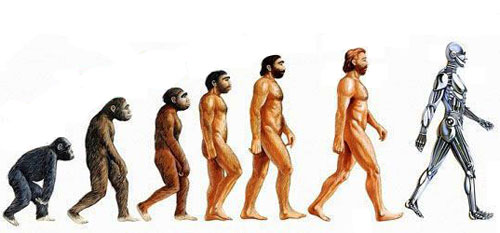
\includegraphics[width=0.8\textwidth]{figures/artificialhumans.jpg}
	\caption{Evolution of bipedalism (artistic depiction from \cite{human_evol_fig})}
	\label{fig:biped_evolution}
\end{figure}

\subsection{Biped motion and engineering} % (fold)
\label{sub:bipedalism_and_engineering}
The discipline of engineering has been historically among the latest of the cited ones to start its contribution to the research and improvement of biped motion in a well defined manner, although its earliest contributions seem to date from ancient Egypt and India \cite{prosthetics_history}.
From the study of human bipedal motion described above, the insights emerged regarding its biomechanical and control functioning together with the need to restore, improve or imitate its capabilities led to the creation of new branches within the discipline of engineering.
The three most relevant ones for the present thesis are listed and introduced below.

\begin{enumerate}
	\item Orthotics
	\item Prosthetics
	\item Artificial legged locomotion 
\end{enumerate}

\paragraph{Orthotics} % (fold)
\label{par:orthotics}
Orthotics is a specialty within the medical field concerned with the design, manufacture and application of orthoses. An orthosis is an externally applied device used to modify the structural and functional characteristics of the neuromuscular and skeletal system, as per definition in \cite{ISO_orthosis}.

Therapeutic models to exoskeletons... 
\todo{Add some more stuff}
% paragraph orthotics (end)

\paragraph{Prosthetics} % (fold)
\label{par:prosthetics}
Prosthetics is the field of medicine that comprises the design and creation of prosthesis, defined as artificial limbs aimed at restoring motor and sensory capabilities in amputee patients.
Since the first lower-limb prosthesis implant recorded in history, documented in the Rigveda \cite{prosthetics_history}, to the current state of the art there has been more than 3000 years of development.
This time has taken prosthetics from single-piece, non-articulated devices with no actuation or sensory feedback to the current near-natural, anthropomorphic structures and control systems adapted to the patient needs and able to closely provide the properties of a biological limb.
As in the orthoses design, the aim of the prosthetics is to mimic as closely as possible the human capabilities with designs such that they adapt to the subject as naturally as possible.
Thus, their development goes parallel to the research and understanding of the human body.
One of the most comprehensive studies in lower-limb prostheses, their design and actuation is the one provided in \cite{grimmer}.
% paragraph prosthetics (end)

\begin{figure}[h]
	\centering
    \begin{subfigure}[b]{0.3\textwidth}
        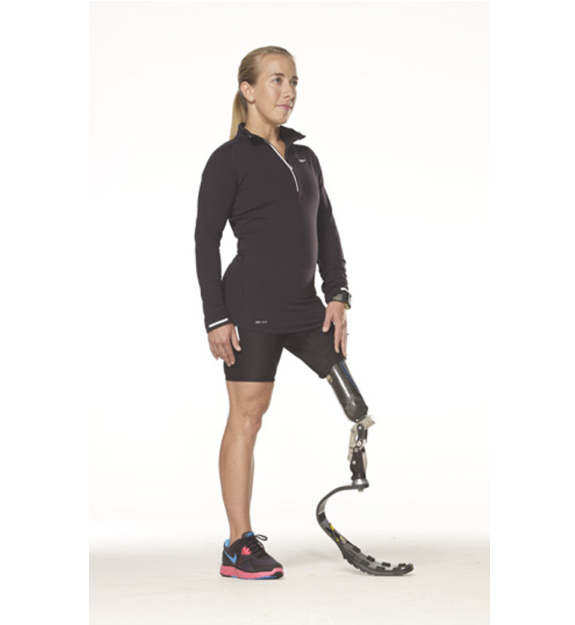
\includegraphics[width=\textwidth]{figures/prosthetic_leg.pdf}
        \caption{Prosthetic leg, Össur Flex-Run}
        \label{fig:prosthetic_leg}
    \end{subfigure}
    \centering
    \begin{subfigure}[b]{0.3\textwidth}
        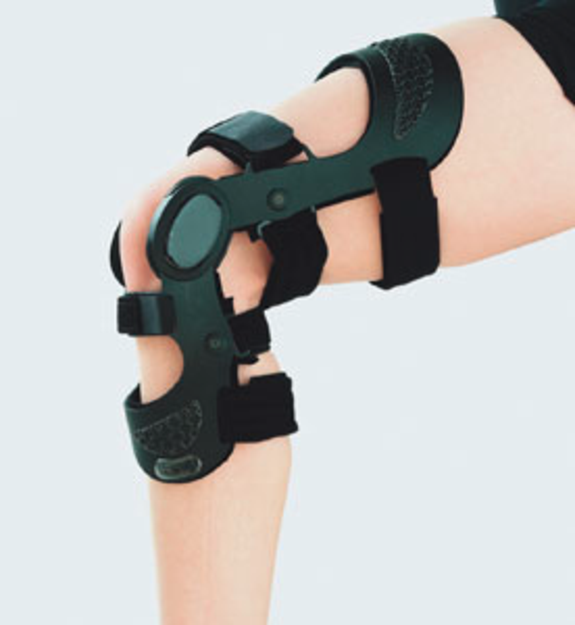
\includegraphics[width=\textwidth]{figures/orthotic_leg.pdf}
        \caption{Knee orthosis, New Hope Co.}
        \label{fig:orthotic_leg}
    \end{subfigure}
    \centering
    \begin{subfigure}[b]{0.3\textwidth}
        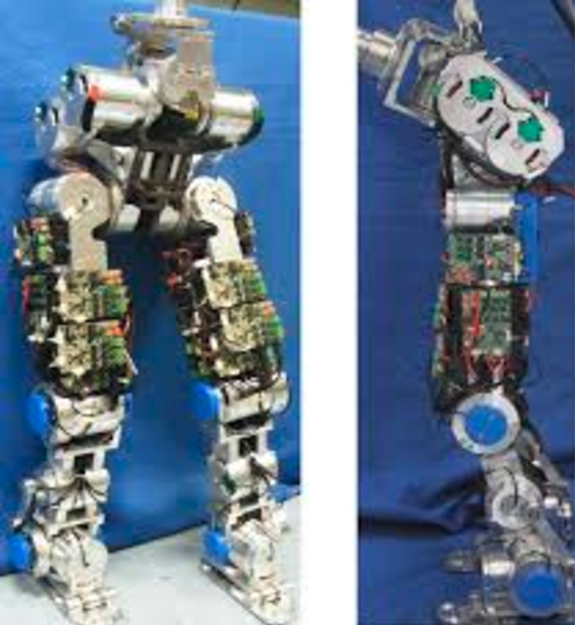
\includegraphics[width=\textwidth]{figures/robotic_leg.pdf}
        \caption{Robotic legs, COMAN robot \cite{coman}}
        \label{fig:robotic_leg}
    \end{subfigure}
\end{figure}

\paragraph{Artificial legged locomotion} % (fold)
\label{par:humanoid_robots}  
The first artificial walking artifacts recorded date from the ancient Greece.
It is in this period when humankind first tries to imitate and replicate the structures found in nature, creating mechanisms to get a deeper knowledge of their functioning and mimic them.
But it is during the Renaissance in Europe when the developments in mechanics and the study of the nature and the human body allows to create the first automata able to walk as a predefined combination of complex mechanical operations.
It is after the Second World War, with the application of electronics and computer technology that the advancement of walking machines is revolutionized \cite{legged_mot_history1}.

The engineering branch of modern robotics has its origins in the second half of the 20th century has a conjunction of the areas of electrical and mechanical engineering and computer science.
However, its interest in achieving resemblance to the locomotion means of both humans and animals  and their capabilities arose in the 1980's.
It first crystallized into the construction of Wabot-1 at WASEDA University or the creation of the Leg Laboratory by Marc Raibert at the Massachusetts Technological Institute.
The purpose of the research in this field was the construction of useful knowledge basis on how human and animal locomotion works that could be used in the creation of legged vehicles, as described in \cite{mit_leg_lab1}.
% paragraph humanoid_robots (end)



% subsection bipedalism_and_engineering (end)


%%!TEX root = ../../report.tex
\chapter{State of the art} % (fold)
\label{cha:state_of_the_art}
%!TEX root = ../../../report.tex
\section{The evolution of bipedalism}
\label{sec:bipedalism}

The current human bipedal locomotion arises from the combination of a wide variety of subsystems working in conjunction to achieve the intended gait generation according to the requirements of the situation.
The biomechanics of the limbs, consisting in bones, muscles and tendons under the control of the nervous system yields the adequate production of the different motion patterns in order to displace the body as energetically efficiently as possible.
This complex behavior is the result of 4 million years of an evolution \cite{bipedalism2} that started in primates and that has entailed both morphological and neurological changes in the human body since the first bipedal hominids to the current structure in Homo sapiens.
There exist several different theories about the reasons that originated and led to the adaption of this posture and bipedal motion.
Although different, most of them assume that most of them assume that the development of this structural and behavioral changes arose from a change in the environment in pre-hominids, for with bipedal behavior suddenly offered some kind of survival value \cite{bipedalism1}.
However, the genus Homo is not the only species that has evolved towards two-legged locomotion
Currently there are a few more species that have reached this method of displacement as a result of a natural selection process in which bipedalism offered the broadest set of advantages of the specie being the main ones listed below. 

\\
\hfill

\begin{itemize}
	\item Erect posture for a wider field of view and reach range.
	\item Free forelimbs, that could evolve towards specialized, non-locomotory applications such as object manipulation, combat, flight, etc.
	\item Faster displacement in certain species, although not generally.
\end{itemize}

Extensive research in the actuation and control structures involved in human bipedalism has been conducted from within the scientific fields of anthropology, biology, medicine, sport science and lately, several areas withing the engineering.
Its goal, as per definition of science, has been to reach a full understanding of what led to this behavior and the knowledge of how it functions, together with the discovery of ways in which it can be mimicked and improved, aiming at a more inexpensive and optimized locomotion.
This last fact has led to the belief that the next stage in the evolution of human locomotion will not come from nature as until nowadays, but from the hand of science and engineering, which has been lately depicted in literature and pop-culture as in \ref{fig:biped_evolution}.

\begin{figure}[h]
	\centering
	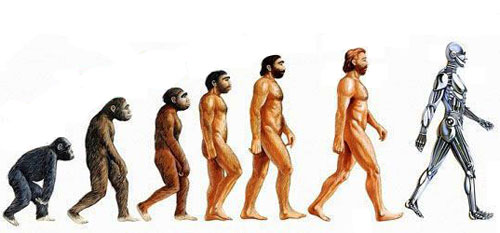
\includegraphics[width=0.8\textwidth]{figures/artificialhumans.jpg}
	\caption{Evolution of bipedalism (artistic depiction from \cite{human_evol_fig})}
	\label{fig:biped_evolution}
\end{figure}

\subsection{Biped motion and engineering} % (fold)
\label{sub:bipedalism_and_engineering}
The discipline of engineering has been historically among the latest of the cited ones to start its contribution to the research and improvement of biped motion in a well defined manner, although its earliest contributions seem to date from ancient Egypt and India \cite{prosthetics_history}.
From the study of human bipedal motion described above, the insights emerged regarding its biomechanical and control functioning together with the need to restore, improve or imitate its capabilities led to the creation of new branches within the discipline of engineering.
The three most relevant ones for the present thesis are listed and introduced below.

\begin{enumerate}
	\item Orthotics
	\item Prosthetics
	\item Artificial legged locomotion 
\end{enumerate}

\paragraph{Orthotics} % (fold)
\label{par:orthotics}
Orthotics is a specialty within the medical field concerned with the design, manufacture and application of orthoses. An orthosis is an externally applied device used to modify the structural and functional characteristics of the neuromuscular and skeletal system, as per definition in \cite{ISO_orthosis}.

Therapeutic models to exoskeletons... 
\todo{Add some more stuff}
% paragraph orthotics (end)

\paragraph{Prosthetics} % (fold)
\label{par:prosthetics}
Prosthetics is the field of medicine that comprises the design and creation of prosthesis, defined as artificial limbs aimed at restoring motor and sensory capabilities in amputee patients.
Since the first lower-limb prosthesis implant recorded in history, documented in the Rigveda \cite{prosthetics_history}, to the current state of the art there has been more than 3000 years of development.
This time has taken prosthetics from single-piece, non-articulated devices with no actuation or sensory feedback to the current near-natural, anthropomorphic structures and control systems adapted to the patient needs and able to closely provide the properties of a biological limb.
As in the orthoses design, the aim of the prosthetics is to mimic as closely as possible the human capabilities with designs such that they adapt to the subject as naturally as possible.
Thus, their development goes parallel to the research and understanding of the human body.
One of the most comprehensive studies in lower-limb prostheses, their design and actuation is the one provided in \cite{grimmer}.
% paragraph prosthetics (end)

\begin{figure}[h]
	\centering
    \begin{subfigure}[b]{0.3\textwidth}
        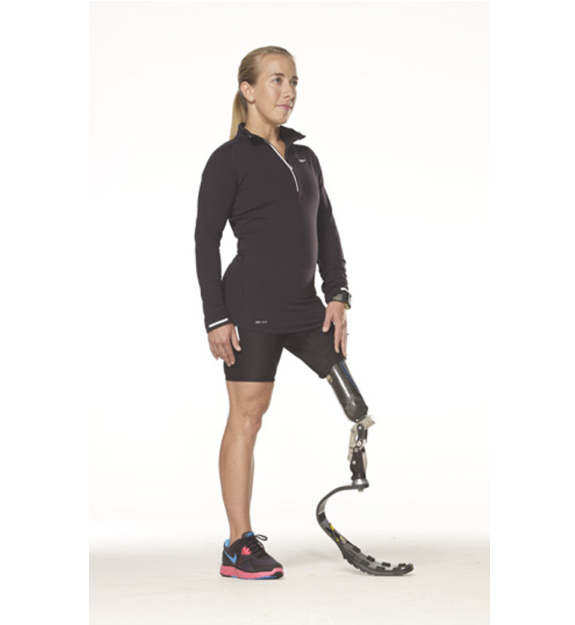
\includegraphics[width=\textwidth]{figures/prosthetic_leg.pdf}
        \caption{Prosthetic leg, Össur Flex-Run}
        \label{fig:prosthetic_leg}
    \end{subfigure}
    \centering
    \begin{subfigure}[b]{0.3\textwidth}
        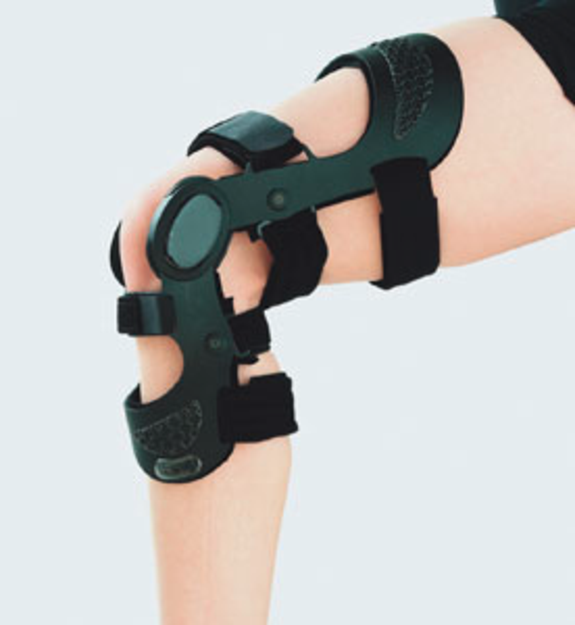
\includegraphics[width=\textwidth]{figures/orthotic_leg.pdf}
        \caption{Knee orthosis, New Hope Co.}
        \label{fig:orthotic_leg}
    \end{subfigure}
    \centering
    \begin{subfigure}[b]{0.3\textwidth}
        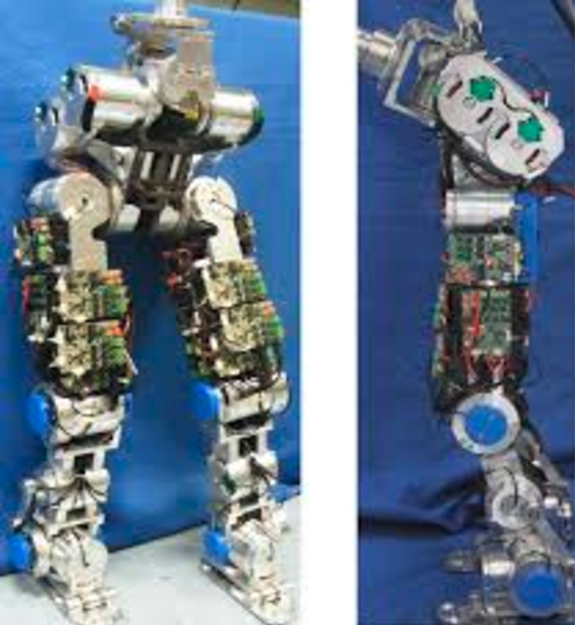
\includegraphics[width=\textwidth]{figures/robotic_leg.pdf}
        \caption{Robotic legs, COMAN robot \cite{coman}}
        \label{fig:robotic_leg}
    \end{subfigure}
\end{figure}

\paragraph{Artificial legged locomotion} % (fold)
\label{par:humanoid_robots}  
The first artificial walking artifacts recorded date from the ancient Greece.
It is in this period when humankind first tries to imitate and replicate the structures found in nature, creating mechanisms to get a deeper knowledge of their functioning and mimic them.
But it is during the Renaissance in Europe when the developments in mechanics and the study of the nature and the human body allows to create the first automata able to walk as a predefined combination of complex mechanical operations.
It is after the Second World War, with the application of electronics and computer technology that the advancement of walking machines is revolutionized \cite{legged_mot_history1}.

The engineering branch of modern robotics has its origins in the second half of the 20th century has a conjunction of the areas of electrical and mechanical engineering and computer science.
However, its interest in achieving resemblance to the locomotion means of both humans and animals  and their capabilities arose in the 1980's.
It first crystallized into the construction of Wabot-1 at WASEDA University or the creation of the Leg Laboratory by Marc Raibert at the Massachusetts Technological Institute.
The purpose of the research in this field was the construction of useful knowledge basis on how human and animal locomotion works that could be used in the creation of legged vehicles, as described in \cite{mit_leg_lab1}.
% paragraph humanoid_robots (end)



% subsection bipedalism_and_engineering (end)


%%!TEX root = ../../report.tex
\chapter{State of the art} % (fold)
\label{cha:state_of_the_art}
\input{chapters/cha_state_of_the_art/Sections/sec_bipedalism_intro}
%\input{chapters/cha_state_of_the_art/cha_state_of_the_art}
%\input{chapters/cha_state_of_the_art/Sections/sec_theoretical_background}
%\section{Theoretical background}



%But it has been in the last 30 years of the past century when the robotics field has started to focus on accomplishing bipedal locomotion, being the first model the WAM-1, built at Waseda University in 1967 \cite{}.
% Since this robot, the evolution of the platforms targeted at mimicking human locomotion has rapidly achieved great successes, which can be exemplified in robots as ASIMO, MABEL or BioBiped \cite{mabel}, \cite{biobiped}, %\cite{}.  
% However, even though the generation of stable walking gaits for biped platforms seems to have reached a next stage with the latest Atlas robot, the variances in kinematics, kinetics and control required for running and for the transition between the walking and running gaits still set out unsolved challenges.
% Besides, differences in energy consumption and balance control or trajectory generation still remain noticeable when comparing the performance of humanoid robots and humans \cite{h7}.

% In order to contribute to the study of stable walking and running gaits generation in bipedal robots, and aiming at providing a new tool to gain new insights on the transition between these gaits, this project offers a new robotic platform for continuing the research in these areas at the University of Southern Denmark.
% The current bipedal robot being utilized at the AI department at the Mærsk Mc-Kinney Møller Institute to benchmark neural controllers for locomotion is the DACbot walking robot, a next generation of RunBot \cite{runbot1} \cite{runbot2}.
% The limitations of this model when trying to approach human-like gait include among others the lack of actuated ankles or compliance in other joints besides the ankles. 
% Furthermore, its fixed structure and the way it was manufactured make modifications for different experiments or even repairs a hard task.
% A new bipedal platform offering a structure easy to modify and repair, low-cost, fully actuated and whose compliant components can be reconfigured, could be a valuable instrument for future studies.
% The RuBi robot, introduced here, wants to be presented as a mean to overcome the above mentioned restrictions and provide these new features. 
% Besides, the possibilities arisen from having two different study platforms in the department include being able to test neural controllers in different robots to observe their adaption, for instance.



%\section{Current research}
% chapter state_of_the_art (end)
%%!TEX root = ../../../report.tex

\section{Theoretical background}
\label{sec:theoretical_background}

%\section{Theoretical background}



%But it has been in the last 30 years of the past century when the robotics field has started to focus on accomplishing bipedal locomotion, being the first model the WAM-1, built at Waseda University in 1967 \cite{}.
% Since this robot, the evolution of the platforms targeted at mimicking human locomotion has rapidly achieved great successes, which can be exemplified in robots as ASIMO, MABEL or BioBiped \cite{mabel}, \cite{biobiped}, %\cite{}.  
% However, even though the generation of stable walking gaits for biped platforms seems to have reached a next stage with the latest Atlas robot, the variances in kinematics, kinetics and control required for running and for the transition between the walking and running gaits still set out unsolved challenges.
% Besides, differences in energy consumption and balance control or trajectory generation still remain noticeable when comparing the performance of humanoid robots and humans \cite{h7}.

% In order to contribute to the study of stable walking and running gaits generation in bipedal robots, and aiming at providing a new tool to gain new insights on the transition between these gaits, this project offers a new robotic platform for continuing the research in these areas at the University of Southern Denmark.
% The current bipedal robot being utilized at the AI department at the Mærsk Mc-Kinney Møller Institute to benchmark neural controllers for locomotion is the DACbot walking robot, a next generation of RunBot \cite{runbot1} \cite{runbot2}.
% The limitations of this model when trying to approach human-like gait include among others the lack of actuated ankles or compliance in other joints besides the ankles. 
% Furthermore, its fixed structure and the way it was manufactured make modifications for different experiments or even repairs a hard task.
% A new bipedal platform offering a structure easy to modify and repair, low-cost, fully actuated and whose compliant components can be reconfigured, could be a valuable instrument for future studies.
% The RuBi robot, introduced here, wants to be presented as a mean to overcome the above mentioned restrictions and provide these new features. 
% Besides, the possibilities arisen from having two different study platforms in the department include being able to test neural controllers in different robots to observe their adaption, for instance.



%\section{Current research}
% chapter state_of_the_art (end)
%%!TEX root = ../../../report.tex

\section{Theoretical background}
\label{sec:theoretical_background}

%\section{Theoretical background}



%But it has been in the last 30 years of the past century when the robotics field has started to focus on accomplishing bipedal locomotion, being the first model the WAM-1, built at Waseda University in 1967 \cite{}.
% Since this robot, the evolution of the platforms targeted at mimicking human locomotion has rapidly achieved great successes, which can be exemplified in robots as ASIMO, MABEL or BioBiped \cite{mabel}, \cite{biobiped}, %\cite{}.  
% However, even though the generation of stable walking gaits for biped platforms seems to have reached a next stage with the latest Atlas robot, the variances in kinematics, kinetics and control required for running and for the transition between the walking and running gaits still set out unsolved challenges.
% Besides, differences in energy consumption and balance control or trajectory generation still remain noticeable when comparing the performance of humanoid robots and humans \cite{h7}.

% In order to contribute to the study of stable walking and running gaits generation in bipedal robots, and aiming at providing a new tool to gain new insights on the transition between these gaits, this project offers a new robotic platform for continuing the research in these areas at the University of Southern Denmark.
% The current bipedal robot being utilized at the AI department at the Mærsk Mc-Kinney Møller Institute to benchmark neural controllers for locomotion is the DACbot walking robot, a next generation of RunBot \cite{runbot1} \cite{runbot2}.
% The limitations of this model when trying to approach human-like gait include among others the lack of actuated ankles or compliance in other joints besides the ankles. 
% Furthermore, its fixed structure and the way it was manufactured make modifications for different experiments or even repairs a hard task.
% A new bipedal platform offering a structure easy to modify and repair, low-cost, fully actuated and whose compliant components can be reconfigured, could be a valuable instrument for future studies.
% The RuBi robot, introduced here, wants to be presented as a mean to overcome the above mentioned restrictions and provide these new features. 
% Besides, the possibilities arisen from having two different study platforms in the department include being able to test neural controllers in different robots to observe their adaption, for instance.



%\section{Current research}
% chapter state_of_the_art (end)
    %!TEX root = ../../report.tex
\chapter{Conception and initial analysis} % (fold)
\label{cha:analysis}
The process of designing and constructing a bipedal robot as the presented here is a task of great magnitude in which a big set of parameters has to be analyzed and determined aiming at the most optimal solution possible\footnote{Optimality here is measured in terms of the aimed goals, described in \ref{sec:goals}.}.
The important role of the geometrical and inertial mechanical parameters in locomotion control was first proved by \cite{passive_walking}, and their relevance deserves a careful study.
Thus, the sections in this chapter contain the conceptual presentation of a set of design criteria and first approaches to the construction of the RuBi prototype arisen from the study of these parameters.

%!TEX root= ../../../report.tex

\section{Bipedal locomotion} % (fold)
\label{sec:bipedal_walking_and_running_gaits}
This section contains a superficial comparative study of the characteristics of human-like walking and running patterns.
The reason is to help justify in the following chapters the decisions taken during the design.

Although walking and running motion patterns in humans might resemble each other at first glance, they contain important variations that imply that a robot able to walk at a certain speed is not necessary capable of running at the same speed, or running at all.
The existence of the so-called "flight phase" in running but not in walking cycles is the main difference between them.
This phase encompasses the period in which there is no contact between the feet and the ground and causes the main variations in energy and trajectory generation.

\subsection{Walking and running gaits comparison} % (fold)
\label{sub:walk_and_run_comparison}
The differences in both joint kinematics and kinetics between both patterns arisen from this distinction are studied in \cite{grimmer}, Manuscript I, for a wide range of speeds.
From the cited paper it can be seen that the joint positions for a whole cycle in both walking and running patterns are very similar, specially for hip and knee.
Furthermore, the joint velocity profiles have almost the same shape but differ in the magnitudes, being higher the angular speeds reached for running.
Similar conclusions can be extracted from a quick comparison between the torque and power profiles in a running and walking cycle.
While the shapes of the functions for the three joints are the really close, with bigger differences for the ankle, the values of the curve are in average smaller for human walking than for running.
As expected, the conclusion is that higher requirements for joint speed, torque and power are expected for running, specially for the knees and the ankles.

% Impact forces comparison here
Besides, the foot strike and impact forces during the landing phase in both cases change, both in intensity and profile. ***

% subsection walk_and_run_comparison (end)

% section bipedal_walking_and_running_gaits (end)
%!TEX root = ../../../report.tex

\section{Geometrical dimensions of the frame} % (fold)
\label{sec:dimensions}
The selection of the final dimensions of RuBi corresponds to an iterative process in which power requirements and achieving human-like kinematics have been the main constraints when assessing the size of the robot.
A first approach was taken from \cite{grimmer}, Manuscript I, where normalized values of power required per joint and per kilogram of the structure can be found.
The first iteration targeted a robot of dimensions $m = 1Kg$ and length from the hip joint to the tip toes of $L = 0.6 m$ for a fully stretched leg.
The final parameters from the last iteration can be found in ***%***chapter Results

Once estimated an overall length of the structure, an initial value of the dimensions of each link were decided to be obtained based on the German section of the ISO 7250-2 \cite{iso_measurements} and the DIN 33402-2 \cite{din_measurements1} norms, following the idea of mimicking human-like motion as closely as possible.
These two norms are standard references in industry and were considered a general enough source of information.
Figure \ref{fig:human_measurements} depicts some of the human dimensions extracted from the norms and applied to the design of RuBi.
Their names and values for male between 18-65 year old and in percentile 50 can be found in table \ref{tab:din_proportions}.

\begin{figure}[h]
	\centering
	\begin{subfigure}[b]{0.3\textwidth}
        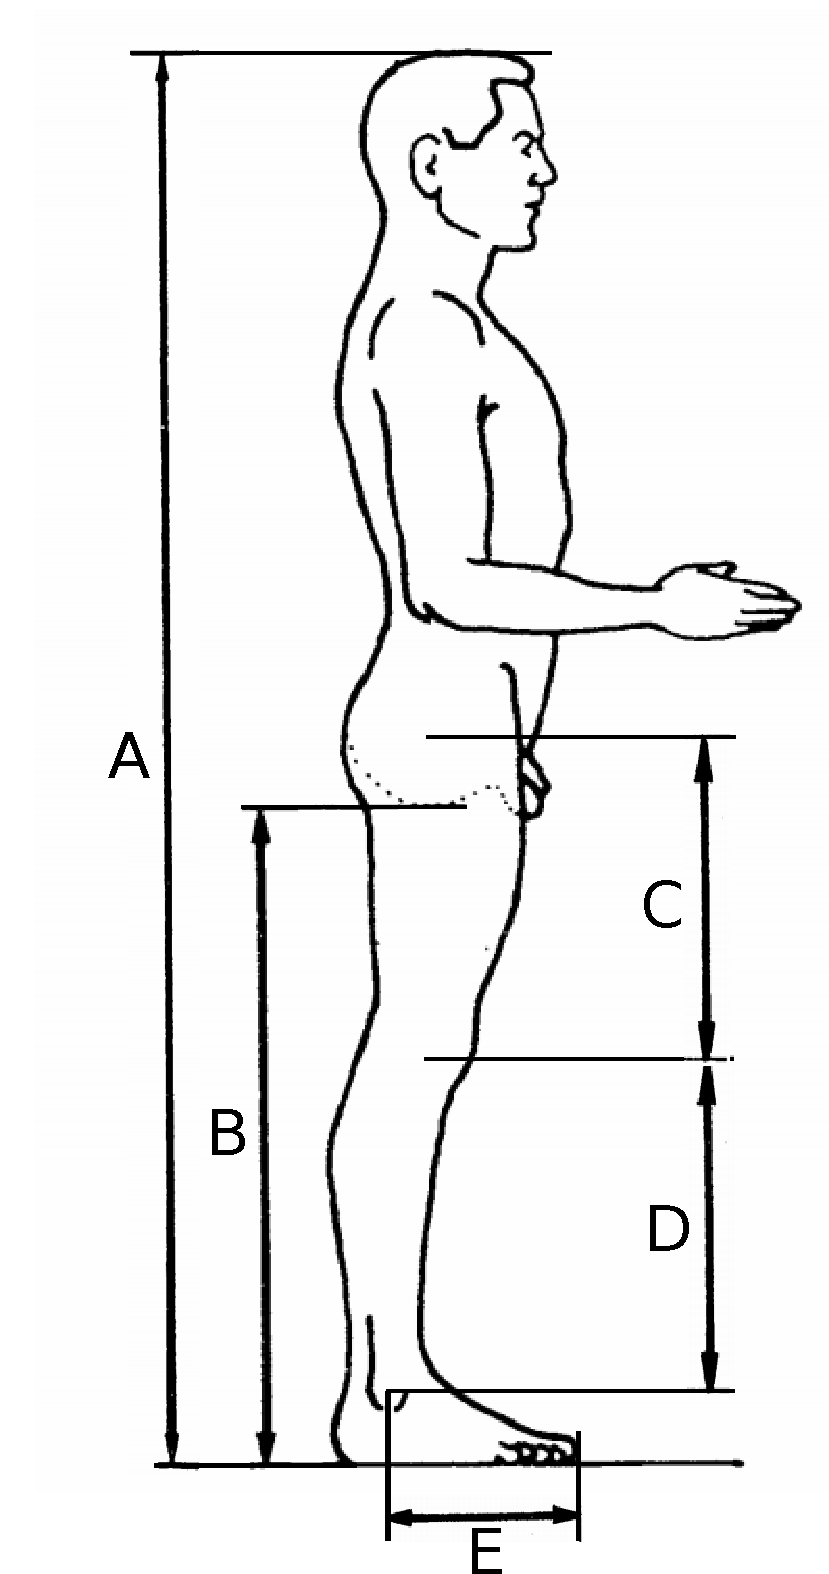
\includegraphics[width=\textwidth]{figures/din_measurements.pdf}
        \caption{Left foot}
        \label{fig:din1}
    \end{subfigure}
    \begin{subfigure}[b]{0.4\textwidth}
        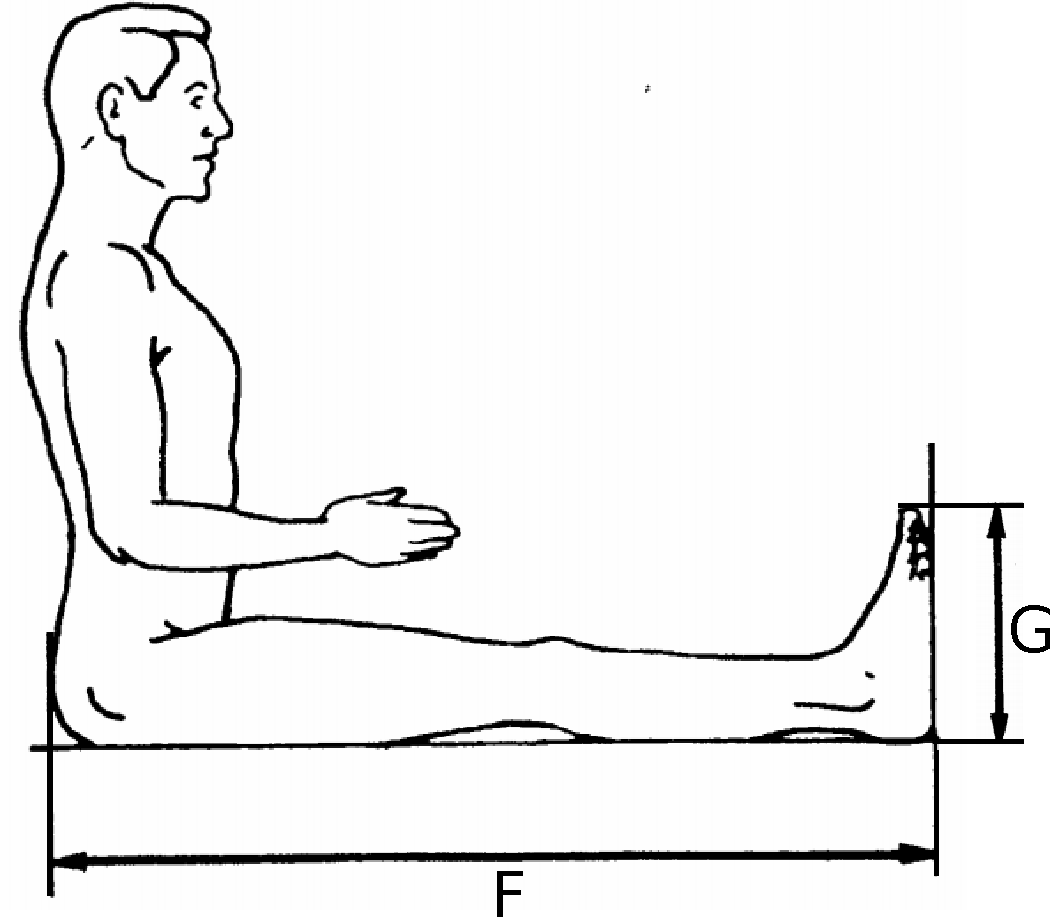
\includegraphics[width=\textwidth]{figures/din_measurements2.pdf}
        \caption{Hip}
        \label{fig:din2}
    \end{subfigure}
	\caption{Lower body measurements used for RuBi. Picture adapted from \cite{din_measurements1}.}
	\label{fig:human_measurements}
\end{figure}


\begin{table}
\begin{center}
	\begin{tabular}{c | c | c | c}
	  Index & Definition & Value & \% of Stature \\
	  \hline
	  A & Stature (body height) & ** & 100 \\
	  B & Crotch height & ** & ** \\
	  C & Femur height & ** & ** \\
	  D & Tibial height & Not in norm & **\\
	  E & Ankle-toe tip distance & Not in norm & ** \\
	  F & Buttocks-leg length & ** & ** \\
	  G & Sole length & ** & **
	\end{tabular}
	\caption{Human proportions from DIN 33402-2}
	\label{tab:din_proportions}
\end{center}
\end{table}

\subsection{Limbs length} % (fold)
\label{sub:limbs_lengths}
The dimensions needed to create a simplified model of one leg are the limbs lengths, which are the straight line distances measured from two consecutive joints.
They have been called $l_{i}$ where $i$ is the robot link + joint as per table \ref{tab:limb_index} and can be seen in Figure \ref{fig:kinematics}.
However, the norm does not determine all of them.

\begin{table}
\begin{center}
	\begin{tabular}{c | c | c}
	  $l_{i}$ & Limb \\
	  \hline
	  $l_{1}$ & Hip + thigh & C \\
	  $l_{2}$ & Knee + Foreleg & D\\
	  $l_{3}$ & Ankle + foot & E 
	\end{tabular}
	\caption{Limbs index}
	\label{tab:limb_index}
\end{center}
\end{table}

Since $C$ and $E$ are not standard measurements in industry, they have been obtained as follows:

\paragraph{The Femur height}
The crotch height, denoted as $B$ in the figure, has been averaged with the buttocks-leg length and the tibial height + an empirical approximation of the height of the ankle have been subtracted from the result, obtaining $C$.

\paragraph{The ankle-toe tip distance}
Since this distance is not standard either, it has been obtained once again adjusting the sole length with empirical measurements.
% subsection limbs_lengths (end)

\subsection{Hip and sole width} % (fold)
\label{sub:subsection_name}
The hip width sitting, as defined in the norm and for the same sample group than before, has been used as starting point to define the final width of the structure of the hip.
This standard measurement has been scaled down to a human of length L from hip joint to toe tip, which would correspond to $L=C+D+E$, using the proportion between stature and lower body lengths, also obtained from the norm.
The same process has been conducted to calculate the implemented width of the foot sole.

% subsection hip_sole_width (end)

No other standard measurement has been used as reference for the design, such as thigh or lower leg circumferences, since they do not affect the kinematics of the structure although they have a big influence in its dynamics.
The criteria followed to model the dynamics of the robot is explained in \ref{sec:physical_properties}.


%% Here we just describe the process followed to obtain the final dimensions. 
%% The final results are shown in Chapter Results --> add tables and Froude number calculus


% section dimensions (end)
%!TEX root = ../../../report.tex

\section{Inertial dimensions of the frame} % (fold)
\label{sec:physical_properties}
This section presents the theoretical guidelines followed during the design of RuBi regarding its dynamic model.
The calculations carried out are to be found in chapters \ref{cha:mathematical_model} and \ref{cha:design}. 
The determination of the geometrical dimensions for a robot model is in general a deterministic task in which all the parameters can be selected without dependencies or limitations.
However the inertial parameters of a robot will be the result of the selection of these dimensions, together with the materials utilized for the implementation and the configuration of the elements on the structure, among others.
Here, the goal of the adjustment of the final inertial parameters is not to mimic the dynamics of human legs as with the kinematics, but to reduce the power requirements for locomotion while ensuring robustness and reliability.
The main inertial parameters object of study here are the mass of the links, the positions of their CoM and their inertia moments.
Other parameters with an influence in the model dynamics such as frictions or delays introduced by transmissions are not discussed here due to the complexity of its determination at this stage of the project.

\subsection{Mass of the limbs} % (fold)
\label{sub:mass_of_the_limbs}
The mass of each limb $i$ will depend on the materials used, their geometry and their density together with any other component added to the link (actuators, electronics, transmissions).
As explained before, keeping the overall mass of the frame as low as possible while guaranteeing the fulfillment of all the structural requirements such as resistance and resilience has been one of the main goals of the analyses conducted in the design of RuBi.
This criteria led to the allocation of the embedded electronics off the robot and aim at small electric actuators as the lightest possible solution for the actuation. 
The calculations to select the limb material and profile are to be found in \ref{sub:limb_profile}.
The final masses per limb have been obtained as an approximate sum of the components that constitute them, due to the complexity of measuring them directly or using system identification techniques. 
They can be seen in %\ref{} reference to Results table and Implementation section
And they have been assumed to be concentrated in the CoM of each link for the computation of the dynamic model.
% subsection mass_of_the_limbs (end) 

\subsection{Centers of mass} % (fold)
\label{sub:centers_of_mass}

\paragraph{Limbs center of mass} % (fold)
\label{par:limbs_center_of_mass}
Limbs center of mass
The position of the center of mass of each limb referred to its joint rotational axis is a function of its masses, their distributions and its geometry.
Their coordinates are given referred to a local reference frame attached to each joint, with its $Z$ axis perpendicular to the sagital plane and its $X$ and $Y$ axes parallel to its equivalents in the main reference frame in the hip, shown in Figure \ref{fig:kinematics}.
Its direct influence in the dynamics of the system is shown in \ref{sec_dynamic_model}, equation \ref{eq:N-E_eq1}.
The coordinates of the CoM of the limbs have been estimated during the design through the 3D CAD design software tool SolidWorks \cite{solidworks}.
Their final values can be found in %\ref{} reference to Results table and Implementation section
% paragraph limbs_center_of_mass (end)

\paragraph{Center of mass of the frame} % (fold)
\label{par:center_of_mass_of_the_frame}
Frame center of mass
The location of the frame center of mass plays a very important role in the stability of the robot \cite{rojas}.
Its theoretical placement when standing still should be in the sagital plane of the structure, as close to the hip as possible, similar to humans (accounting that there is no torso).
A robust locomotion should result in a controlled and limited motion of the CoM. 
A high positioning of the CoM in the structure would make it more sensitive to the actuators influence, allowing a better balance control, while a lower placement in the structure could increase its robustness against inertial phenomenas.
The trade-off between these two criteria has been tried to be found.
As for the limbs, the coordinates of the CoM of the structure have been computed through SolidWorks and their final values can be found in %\ref{} reference to Results table and Implementation section

% paragraph center_of_mass_of_the_frame (end)
% subsection centers_of_mass (end)

\subsection{Moments of inertia} % (fold)
\label{par:moments_of_inertia}
The inertia moments of each limb will be the result of the distribution of the masses with respect to the joint axis.
Keep the CoM close to the joints to reduce them!--> smaller torque required for same angular accelerations***


% subsection moments_of_inertia (end)



%Friction model and transmissions delays not included because of its complexity

% section physical_properties (end)
%!TEX root = ../../../report.tex
\section{Joints} % (fold)
\label{sec:joints}

\begin{figure}[ht!]
  \centering
  \includegraphics[width=\textwidth]{figures/20160518_195014.jpg}
  \caption{Might help}
  \label{fig:figure1}
\end{figure}

  \subsection{Actuators} % (fold)
  \label{sub:actuators}

  %Need of angular motion for the joints: possible ways of generating it?

  % subsection actuators (end)

  \subsection{Transmission} % (fold)
  \label{sub:transmission}

  %Reduction of the moments of inertia
  %Introduction of delays and loss of accuracy 

  % subsection transmission (end)

  \subsection{Compliance} % (fold)
  \label{sub:compliance}

  %Flexible vs stiff drive train
  %Power peak and average consumption comparisons 


  \begin{figure}[hb!]
    \begin{subfigure}{.19\textwidth}
      \centering
      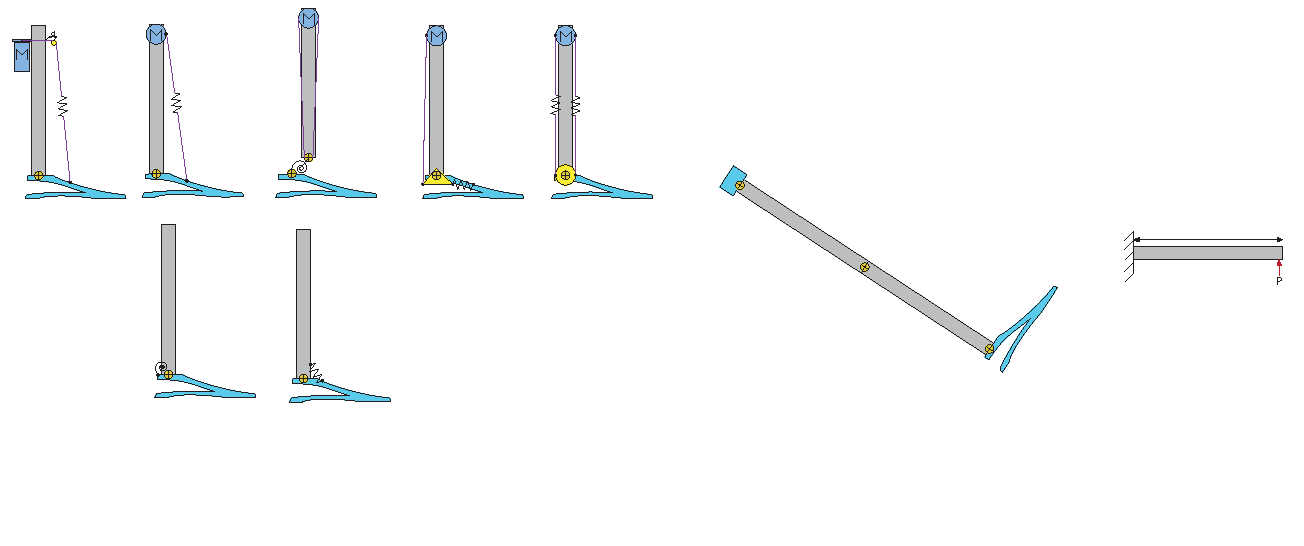
\includegraphics[width=\linewidth]{figures/illustration_serial_pulley.pdf}
      \caption{Serial pulley}
      \label{fig:series_pulley}
    \end{subfigure}
    \begin{subfigure}{.19\textwidth}
      \centering
      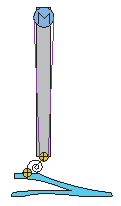
\includegraphics[width=\linewidth]{figures/illustration_serial_rotational.pdf}
      \caption{Series rotational}
      \label{fig:series_rotational}
    \end{subfigure}
    \begin{subfigure}{.19\textwidth}
      \centering
      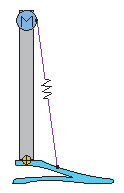
\includegraphics[width=\linewidth]{figures/illustration_serial_direct_i.pdf}
      \caption{Series direct 1}
      \label{fig:series_direct_i}
    \end{subfigure}
    \begin{subfigure}{.19\textwidth}
      \centering
      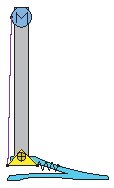
\includegraphics[width=\linewidth]{figures/illustration_serial_direct_ii.pdf}
      \caption{Series direct 2}
      \label{fig:series_direct_ii}
    \end{subfigure}
    \begin{subfigure}{.19\textwidth}
      \centering
      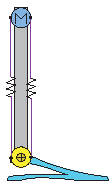
\includegraphics[width=\linewidth]{figures/illustration_serial_elastic_band.pdf}
      \caption{Series elastic band}
      \label{fig:series_elastic_band}
    \end{subfigure}
  \end{figure}  

  % subsection compliance (end)

% section joints (end)

% chapter analysis (end)
    %!TEX root = ../../report.tex
\chapter{Mathematical model of RuBi} % (fold)
\label{cha:mathematical_model}

The motivation to start the development of the mathematical model was the seek of a set of equations with which calculating the requirements for the actuators could be easily achievable.
This task finally evolved towards the construction of a simple dynamic model of the robot and the formulation of the vertical jump dynamics case.
The main goal was to compute the values of the necessary parameters to select joint actuators able to keep up with the requirements of the application.
However, by definition, to do so the application needed to be defined to the extent that these dimensions could be obtained.
Thus, this chapter contains the definition of the task RuBi is expected to be able to perform, the control model defined for it and an explanation of the assumptions made in order to simplify the resulting model. 
After, the necessary kinematic model of the robot is presented as an intermediary step to compute the simplified dynamic model of the robot, which is introduced next to it.
All the algorithms described in this chapter have been implemented in MATLAB and the scripts can be found in the source folder attached to this report.

\section{Actuators}
\label{sec_actuators}
%!TEX root = ../../../report.tex

\section{Analysis of vertical jump} % (fold)
\label{sec:jumping_case}
Modeling the dynamics of walking gaits in a bipedal robot with 6 DOF has proved significantly complex and time consuming, even for the planar case.
However, it is essential for the obtainment of the most extreme torque and velocity values to apply to each joint during the motion, necessary to gauge the required actuators for the application.
In order to ease the task, instead of calculating the motion equations for the walking or running cases, it was resolved to model the dynamics of the vertical jump case.
This was decided under the assumption that a structure able to perform a static, vertical jump of a certain height $h$ and determined characteristics on one leg could be able to fulfill the power requirements necessary for running, both from an actuation and a structural point of view.
This assumption was built upon the findings introduced in \cite{jump-run1} and \cite{jump-run2}.

\subsubsection{Vertical jump dynamics} % (fold)
\label{ssub:static_jumping_dynamics}
As explained in section \ref{sec:dimensions}, the dimensions of the robot and its parameters have been conceived to imitate human characteristics and capabilities.
Therefore the jump analysis here will be carried out in resemblance of the human case, based on \cite{jump-dynamics1} and aiming at applying the results to a robot platform, as in \cite{jump-dynamics2}.
The jump case analyzed here can be described according to \cite{jump-dynamics1} as a static, squat jump over one foot with take-off and without counter-movement (SJ-NAS).
Three assumptions have been made regarding the bodies in contact during the landing phase of the robot:

\begin{itemize}
    \item No slipping occurs
    \item Absence rebounding 
    \item There are no structural deformations 
\end{itemize}

The whole jump cycle has been divided into two phases with different analysis: an impulse and an aerial period.

\begin{figure}[ht!]
    \centeringx
    \begin{subfigure}[b]{0.3\textwidth}
        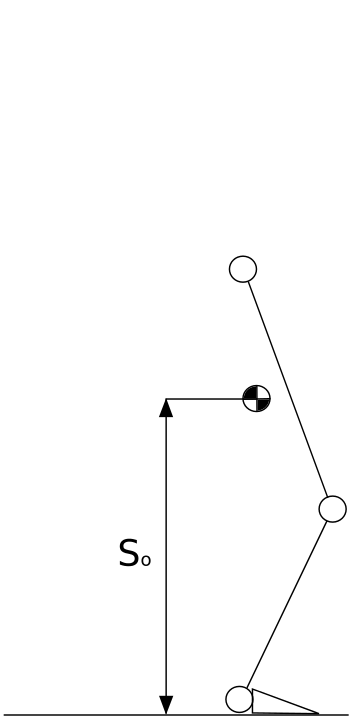
\includegraphics[width=\textwidth]{figures/launch_phase.png}
        \caption{Launch phase}
        \label{fig:launch_phase}
    \end{subfigure}
    \begin{subfigure}[b]{0.3\textwidth}
        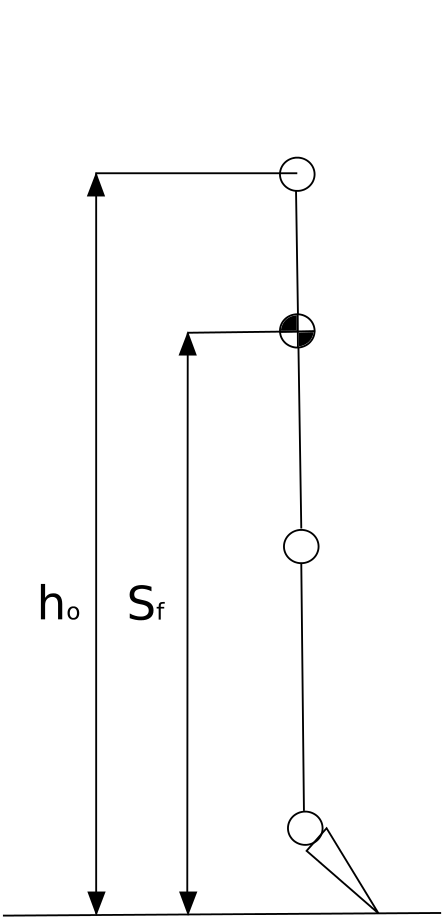
\includegraphics[width=\textwidth]{figures/takeoff_phase.png}
        \caption{Takeoff phase}
        \label{fig:takeoff_phase}
    \end{subfigure}
    \begin{subfigure}[b]{0.3\textwidth}
        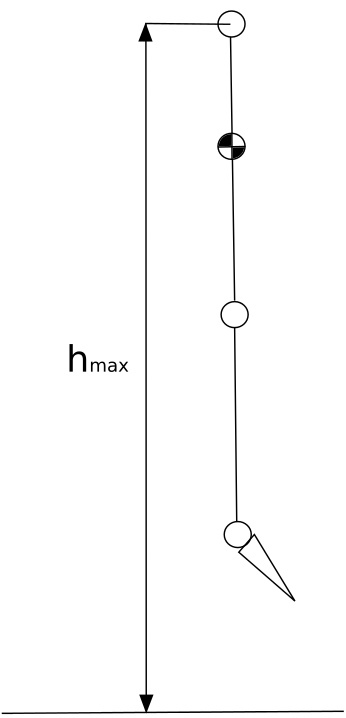
\includegraphics[width=\textwidth]{figures/flight_phase.png}
        \caption{Aerial phase}
        \label{fig:aerial_phase}
    \end{subfigure}
    \caption{Jump phases without fall and landing}
    \label{fig:jump_phases}
\end{figure}


\paragraph{The aerial phase}
The period from the take-off of the toes to the instant in which the maximum height $h_{max}$ has been reached, which can takes place between the instants represented in \ref{fig:takeoff_phase} and \ref{fig:aerial_phase}. 
The rest of the cycle, including fall and landing are not described here.
During the whole period the robot is considered a rigid solid.
This phase is analyzed following the equations of a static projectile motion for the vertical launch case, expressed in \ref{eq:vertical_motion} and \ref{eq:vertical_energy}.

%\begin{equation}
%\label{eq:vertical_motion}	
%	h(t) = V_o t sin(\theta) - \cfrac{1}{2} g t^2 
%\end{equation}

\begin{equation}
\label{eq:vertical_energy}
	m g \Delta h = \cfrac{1}{2} m \Delta V^2
\end{equation}

The equation \ref{eq:vertical_energy} is an energy balance analysis for the flight phase, that can be rearranged as showed in \ref{eq:deltaV}

\begin{equation}
\label{eq:deltaV}
	\Delta V = \sqrt{2 g \Delta h}
\end{equation}

This equation can be used to input the desired displacement in the CoG of the robot during the free flight period and obtain the necessary velocity at take-off $V_{toff}$, which is the one the robot has to reach in the impulse phase.
This can be done since $V_{final} = 0$ and therefore $\Delta V = V_{toff}$.

\paragraph{The impulse phase}
From the initial position at the beginning of the jump, depicted in \ref{fig:launch_phase}, to the instant when the toes of the standing foot take off the ground and the ground reaction force ceases, shown in \ref{fig:takeoff_phase}.
The change in momentum in the robot, of mass $m$, caused by the application of a vertical force with the foot to the ground $F$ during a period $t$ is given by equation \ref{eq:impulse}, derived from the second law of motion of Newton.

\begin{equation}
\label{eq:impulse}
	F  t = m  \Delta V	
\end{equation} 

Substituting equation \ref{eq:deltaV} in \ref{eq:impulse}, the necessary impulse to reach the desired maximum height can be computed.
However, since the force applied to the mass and the application period cannot be decoupled from the result of the equation, an energy analysis has to be carried out together with a posterior optimization of the two values for the desired design of the robot.
Solving equation \ref{eq:impulse} for a small range of application time values and after computing \ref{eq:deltaV} with increasing values of $\Delta h$ in the range $[0.01,0.1]$ meters yields a reciprocal graph whose positive quadrant can be seen in Figure \ref{fig:f-t}

\begin{figure}[ht!]
	\centering
	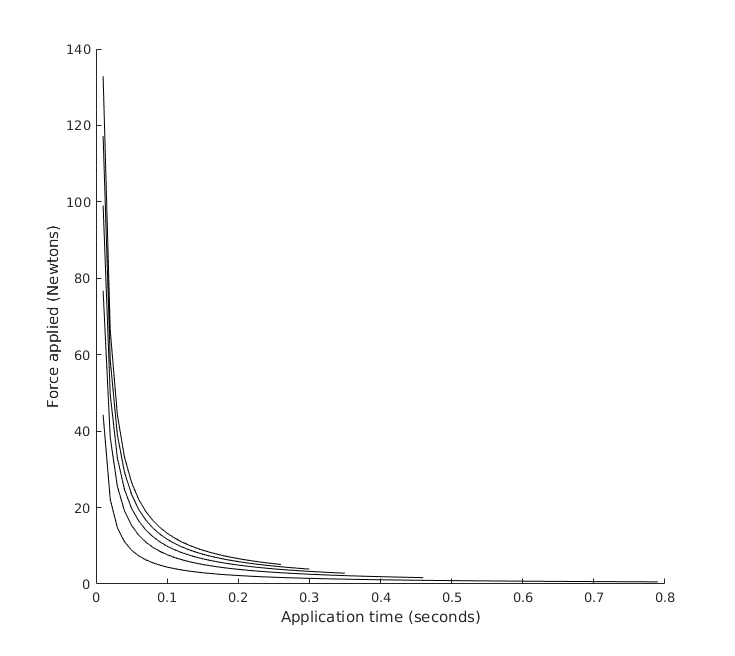
\includegraphics[width=0.8\textwidth]{figures/force-timePlot.png}
	\caption{Force-application time values for the same work magnitude}
	\label{fig:f-t}
\end{figure}

However, the obtained graphs do not propagate to an infinite value of application time, existing a boundary farther than which, the impulse will not produce enough variation in the momentum to launch the body.

\begin{equation}
\label{eq:work}
	W = \int_{t_{toff}}^{t_{f}} F(t)\,\mathrm{d}t = \cfrac{1}{2} m \Delta V^2 = F_{min} S
\end{equation}

Equation \ref{eq:work} describes how the work performed by the robot during the impulse phase can relate to the change in its kinetics energy. 
This equation, derived also from Newton's second law would only apply to rigid bodies without internal degrees of freedom, which is not the case.
However, it has been assumed that the displacement given by $S$ is the vertical translation of the CoM of the robot during the impulse and that it is small enough to be a valid assumption in order to use this procedure.
From Figure \ref{fig:jump_phases}, the displacement of the CoM during the impulse is given as $S=S_{f}-S_{o}$.
Knowing the value of $S$, the minimum necessary force can be obtained, and hence its corresponding application time on Figure \ref{fig:f-t} for a given $\Delta h$.
The displacement of the CoM, $S$ will depend on the initial configuration of the robot prior starting the impulse, and its final one.
Furthermore, for a given $\Delta h$, a range of possible values of the ground reaction Force $F$ can be computed within the limits established and a time can be obtained.
Thus, for a determined $\Delta h$ and $t$ values, a $F$ has to be applied by the foot again the ground.
In order to translate that force to joint effort, the dynamic model of the robot is required.

% subsubsection static_jumping_dynamics (end)

% section The_jumping_case (end)
%!TEX root= ../../../report.tex

\section{Kinematic model}
\label{sec_kinematic_model}
The kinematics model of the robot describes the motion of every joint in time disregarding dynamic parameters.
It is used here to compute position, velocity and acceleration of the limbs for given trajectories of the toes, which are the contact point with the ground in the presented study case, through their forward kinematics.
Also the inverse kinematic model is constructed as a tool for the posterior computation of the dynamics model and its application to model the necessary actuators.
The model has been obtained through direct application of trigonometry instead of using the D-H parameters given its simplicity.
To do so, as explained before the case has been reduced to a two-dimensional study of one leg, where each robot leg haS been analyzed as a kinematic chain of three degrees of freedom.
The main reference frame has been placed attached to the hip with its Y axis parallel to the ground, as if this was the base of a robotic arm, and the toe was the tool, has shown in Figure \ref{fig:kinematics}.
This representation has been chosen to ease the construction of the mathematical model.

%%add world reference frame attached to the ground for flight phase study
\begin{figure}[ht]
	\centering
	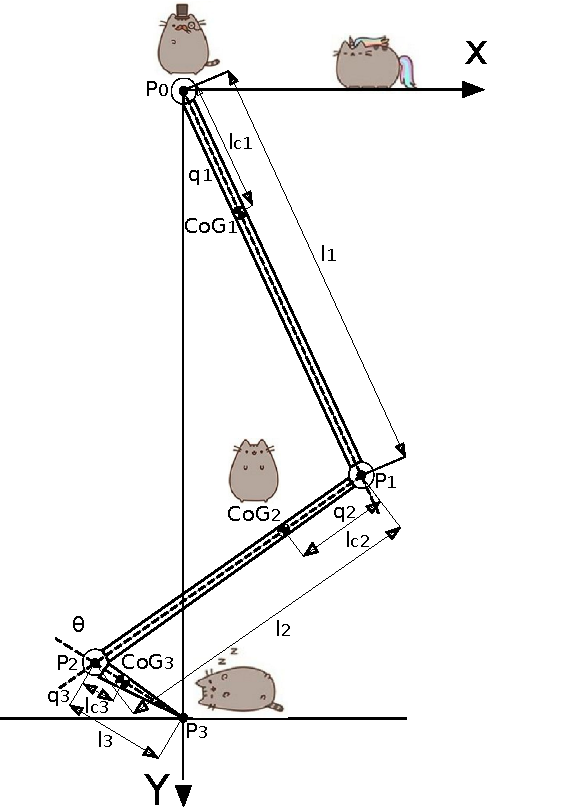
\includegraphics[width=0.4\textwidth]{figures/kinematics_model_kitties.pdf}
	\caption{Coordinate definitions for the schematic model of one leg}
	\label{fig:kinematics}
\end{figure}

The figure above depicts the schematic representation of only one leg, since the other one is equivalent. 
The system is said to be in single support phase since there would be just one foot in contact to the ground.
In the analyzed case, the swinging leg (not represented in Figure \ref{fig:kinematics}) would be static and could be considered an additional link with no degrees of freedom.
The variables $q_{i}$ represent the angles of the joints with respect to their fully-stretched positions to simplify the obtainment of the forward kinematic model, while the angle $\Theta$ is used to express the orientation of the ankle in an absolute manner. 
From Figure \ref{fig:kinematics}, the forward kinematic model in \ref{eq:forward_kinematics} can be easily obtained.


\begin{equation}
\label{eq:forward_kinematics}
	\begin{aligned}
		x_{0} &= 0 \\
		y_{0} &= 0 \\
		x_{1} &= l_{1} \sin(q_{1}) \\
		y_{1} &= l_{1} \cos(q_{1}) \\
		x_{2} &= l_{1} \sin(q_{1}) + l_{2} \sin(q_{1}+q_{2}) \\
		y_{2} &= l_{1} \cos(q_{1}) + l_{2} \cos(q_{1}+q_{2}) \\
		x_{3} &= l_{1} \sin(q_{1}) + l_{2} \sin(q_{1}+q_{2}) + l_{3} \sin(q_{1}+q_{2}+q_{3}) \\
		y_{3} &= l_{1} \cos(q_{1}) + l_{2} \cos(q_{1}+q_{2}) + l_{3} \cos(q_{1}+q_{2}+q_{3}) 
	\end{aligned}
\end{equation}

The variables $x_{i}, y_{i}$ represent the position coordinates of the joints in the right leg, named $P_{i}$ in the schematic in Figure \ref{fig:kinematics} and $P'_{i}$ for the left leg (not depicted).
Once computed, the linear velocity and acceleration of every joint can be obtained by derivation of the forward kinematic model and represented as $\dot{P}_{i}$ and $\ddot{P}_{i}$.

%Add space state vector

The model presented is the most basic one and does not contain the degrees of freedom that could be introduced by springs in the actuators.
This is due to two reasons:

\begin{itemize}
	\item Their configuration can be changed to series, parallel or none in both knees and ankles.
	\item The study of the jump case regarding the parameterization of the actuators has been carried out in the most disadvantageous scenario from the energetic point of view, which in this case means no springs.
\end{itemize}

Following the same approach, the inverse kinematic model can be computed for the right leg, yielding equation \ref{eq:inverse_kinematics}.


\begin{equation}
\label{eq:inverse_kinematics}
	\begin{aligned}
		x_{2} &= x_{3} - l_{3} \sin(\Theta) \\
		y_{2} &= y_{3} - l_{3} \cos(\Theta) \\
		q_{1} &= \arctan \left(\frac{x_{2}}{y_{2}}\right) - \arccos \left(\frac{x_{2}^2 + y_{2}^2 + l_{1}^2 - l_{2}^2}{2 l_{1} \sqrt{x_{2}^2 + y_{2}^2}}\right) \\
		q_{2} &= \pi - \arccos \left(\frac{l_{1}^2 + l_{2}^2 - x_{2} - y_{2}}{2 l_{1} l_{2}}\right) \\
		q_{3} &= \Theta - q_{1} - q_{2} \\
	\end{aligned}
\end{equation}

And equivalently to the forward kinematics, the inverse kinematic model can be derived to obtain the velocities and accelerations in the joint space $\dot{q_{i}}$ and $\ddot{q_{i}}$.

%!TEX root= ../../../report.tex
\section{Dynamic model}
\label{sec_dynamic_model}
The goal of this step is to calculate the relationship between an external force applied to the toe (ground reaction force while jumping) and the necessary torques in the joints for dealing with that external disruption.
This relation can be expressed as a set of second order differential equations represented for the general case as in equation \ref{eq:dynamics_eq1}. 

\begin{equation}
	\label{eq:dynamics_eq1}
	B(q)\ddot{q} + C(q,\dot{q})\dot{q} + g(q) = \tau
\end{equation}

Where $B(q)$ is the inertia matrix, $c(q,\dot{q})$ contains the centrifugal and coriolis acceleration terms and $g(q)$ represents gravity, as in \cite{dynamics1} and \cite{dynamics2}. 
It must be remarked here that the constructed model does not introduce joint friction terms.
For an open kinematic chain as this, three methodologies to obtain the above equation where object of study:

\begin{itemize}
	\item A simplified Euler-Lagrange algorithm, as introduced in \cite{E-L1}, which makes use of the Lagrangian formulation to describe the behavior of the system through work and energy.
	\item The so called Energy Method, presented in \cite{asada} and consisting in finding the relation between the force in the end-effector and the joint torques through the Jacobian of the kinematic chain.
	\item The Newton-Euler algorithm, through which the dynamics of the system can be expressed in terms of forces and moments applied in each member of the chain.
\end{itemize}

It was finally decided to apply the third option due to the fact that it was faster to implement than the E-L algorithm and more reliable than the Energy method.
The Newton-Euler algorithm is founded in classical mechanics and its a recursive method that computes in two steps the velocities and accelerations of every component of a kinematic chain and their forces and torques on the joints.
In \ref{eq:N-E_eq1}, the equations of motion for an individual link are shown.

\begin{equation}
\label{eq:N-E_eq1}
	\begin{aligned}
		f_{i-1, i} - f_{i,i+1} + m_{i} g - m{i} \dot{V}_{ci} =& 0 \\
		N_{i - 1 , i} - N_{i , i + 1} - ( r_{i - 1 , i} + r_{i , Ci} ) \times f_{i - 1 , i} + ( - r_{i , Ci} ) \times ( - f_{i , i + 1}) - I_{i} \dot{\omega_{i}} - \omega_{i} \times ( I_{i} \omega_{i} ) =& 0 \\
		i = 1,..., N 
	\end{aligned}
\end{equation}

These equations contain the coupling forces and moments applied to the link by the immediate ones, however, they cannot be used with them. 
$\omega_{i}$ and $\dot{\omega_{i}}$ represent respectively the angular velocity and acceleration vectors of link $i$ and can be obtained from the joint velocities and accelerations, computed in the previous section, as in equation \ref{eq:angular_magnitudes}.
$I_{i}$ are the inertia matrices of the links, calculated in SolidWorks for the final design of Rubi.

\begin{equation}
\label{eq:angular_magnitudes}	
	\begin{aligned}
		\omega_{i} &= \omega_{i-1} + \xi_{i}\dot{q}_{i}Z_{base}^i\\
		\dot{\omega_{i}} &= \dot{\omega_{i-1}} + \xi_{i}[\ddot{q}_{i}Z_{base}^i + \dot{q}_{i}\omega_{i-1} \times Z_{base}^i]
	\end{aligned}
\end{equation}

The closed-form equations must be derived from them so that they can be applied to the algorithm.
This is done by substituting the coupling forces in the final set of 6 equations obtained for $N=3$ and substituting \ref{eq:torques} in the resulting equations.

\begin{equation}
\label{eq:torques}
	N_{i - 1 , i} = \tau_{i}
\end{equation}

Equation \ref{eq:torques} is valid only for the planar case.
After these steps, a set of three equations of the form \ref{eq:dynamics_eq1} is obtained. 
As parameters, they contain the masses of the links, their vectorial positions, the gravity term and their inertia matrices. 

\todo{add final motion equations?}

This set of equations calculates the necessary torques on the joints as a function of the joints displacements and the external forces and torques applied on the system, as represented in \ref{eq:tau_q}.

\begin{equation}
\label{eq:tau_q}
	\tau(t)_{i} = f(q_{i}(t), \dot{q}_{i}(t), \ddot{q}_{i}(t), \tau_{ext}, F_{ext})
\end{equation}

However, in order to use it the functions that model the trajectories of joints in the joint space must be approximated.
For the ideal static, vertical jump case under study here, the movement of the toe has been constrained to a vertical displacement along the $Y$ axis in order to simplify this task.
Thus, the trajectory of the end-effector of the kinematic chain, $P_{3}$ in Figure \ref{fig:f-t}, can be easily approximated as a function of the form shown in 

\begin{equation}
\label{eq:toe_trajectory}
	\begin{aligned}
	x_{3}(t) &= 0 \\
	y_{3}(t) &= Y_{3}(t_{o}) + \cfrac{Y_{3}(t_{f}) - Y_{3}(t_{o})}{(t_{f} - t_{o}) (t - t_{o})} \\
    \theta(t) &= \theta(t_{o}) + \cfrac{\theta(t_{f}) - \theta(t_{o})}{(t_{f} - t_{o}) (t - t_{o})} 
    \end{aligned}
\end{equation}

Therefore, if equation \ref{eq:toe_trajectory} is used as the input to the inverse kinematic model, the joint displacements will become dependent on the linear displacement of $P_{3}$, and equations \ref{eq:tau_q} will be rewritten as \ref{eq:tau_p}.

\begin{equation}
\label{eq:tau_p}
	\tau(t)_{i} = f(P_{3}(t), \tau_{ext}, F_{ext})
\end{equation}






%!TEX root= ../../../report.tex

\section{Springs influence in the actuators}
\label{sec_springs}
This section deals with the calculations carried out in order to model the influence of the implemented compliance in terms of energy efficiency and joint torque requirements.
As explained in \ref{sec:joints}, the selection of the elastic actuators installed and their configuration on RuBi has been left as a customizable feature for research purposes.
This, together with the fact that RuBi has not been designed to optimize a specific type of gait made pointless the calculation of optimal values of springs.
Thus, the following is just a theoretical frame presented to provide an easy method to compute the influence of the springs in the performance once the user has selected them.
It was meant to be used for the experiments devised on compliance influence in hopping motion, presented in \ref{cha:experiments}.

\subsection{Torque and energy contribution of passive actuators} % (fold)
\label{sub:torque_contribution_of_passive_actuators}
All the springs that can be implemented in RuBi are torsional, as shown in \ref{sub:spring_integration}, whose general equations for torque and energy storage are shown in \ref{eq:torsion_spring}. 

\begin{equation}
\label{eq:torsion_spring}
\begin{aligned}
	\tau_{S} &= -K \Delta \theta \\
	U_{S} &= \frac{1}{2}K \Delta \theta^2
\end{aligned}
\end{equation}

The contribution of the springs torques to the system actuation is therefore modeled introducing the torque equation in \ref{eq:torsion_spring} on the right side of \ref{eq:dynamics_eq1}, which would yield equation \ref{eq:dynamics_eq2}.
Where the torques vector has been divided into the motors and springs inputs.

\begin{equation}
	\label{eq:dynamics_eq2}
	B(q)\ddot{q} + C(q,\dot{q})\dot{q} + g(q) = \tau_{M} + \tau_{S}
\end{equation}

The values of $\Delta \theta_{i}$ can be obtained through forward kinematics for given trajectories, while $\tau_{i}$ can be computed from equation \ref{eq:dynamics_eq1} given the ground contact force model, which is the only external force applied to the system.
Thus, the first formula in \ref{eq:torsion_spring} can be used to calculate the optimal $K$ for a desired joint trajectory and force model, for instance.
Knowing $k_{i}$ and $\Delta \theta_{i}$, the energy stored per gait cycle by each spring can be computed and utilized for studying their influence on the performance of the robot.

\subsection{Joint kinetics} % (fold)
\label{sec:joint_kinetics}
The motor power requirements for each joint can be calculated through equation \ref{eq:motor_power} for direct drive transmission.
This formula does not include inertias, frictions or any other efficiency coefficients. 

\begin{equation}
\label{eq:motor_power}
	P_{m} = \dot{\theta}_{m} \tau_{m}
\end{equation}

By definition of \ref{eq:motor_power}, the value of $P_{m}$ can be positive (motor thrusting) or negative (motor dumping).
Thus, the peak power in the motion cycle can be computed as the its maximum absolute value.
Besides, the equation of motor power is used in \ref{eq:energy_requirement} for calculating the overall energy requirements for a whole motion cycle, employing only absolute values as well.

\begin{equation}
\label{eq:energy_requirement}
 	E_{cycle} = \int{P_{m+}(t) dt} + \int{P_{m-}(t) dt}
 \end{equation} 

\subsubsection{Influence of elastic actuation} % (fold)
\label{sub:influence_of_elastic_actuation}
The above presented are general formulations.
However, the introduction of elastic transmission between motor and load through springs modify the computation of motor power.
The changes resulting from implementing the configurations shown in Figure \ref{fig:sea}, \ref{fig:pea} and \ref{fig:sea_pea} yield equations \ref{eq:SEA_power}, \ref{eq:PEA_power} and \ref{eq:SEA_PEA_power} respectively, as per \cite{grimmer}.
For a complete and detailed description of the parameters in these equations, the reader is referred to the cited paper.

\begin{equation}
\label{eq:SEA_power}
	P_{m} = \tau_{m} \left(\dot{\theta}_{t} + \frac{\dot{M}_{ex}}{K_{s}}\right)
\end{equation}

\begin{equation}
\label{eq:PEA_power}
	P_{m} = (F_{ex} + (K_{p} \Delta \theta_{t})) \dot{\theta}_{t}
\end{equation}

\begin{equation}
\label{eq:SEA_PEA_power}
	P_{m} = \left(F_{ex} + (K_{p} \Delta \theta_{m}) \left(\theta_{t} + \frac{\dot{F}_{ex}}{K_{s}}\right)\right)
\end{equation}

% subsubsection influence_of_elastic_actuation (end)

% section joint_kinetics (end)
% %!TEX root= ../../../report.tex

% \section{Joint kinetics} % (fold)
% \label{sec:joint_kinetics}
% The motor power requirements for each joint can be calculated through equation \ref{eq:motor_power} for direct drive transmission.
% This formula does not include inertias, frictions or any other efficiency coefficients. 

% \begin{equation}
% \label{eq:motor_power}
% 	P_{m} = \dot{\theta}_{m} \tau_{m}
% \end{equation}

% By definition of \ref{eq:motor_power}, the value of $P_{m}$ can be positive (motor thrusting) or negative (motor dumping).
% Thus, the peak power in the motion cycle can be computed as the its maximum absolute value.
% Besides, the equation of motor power is used in \ref{eq:energy_requirement} for calculating the energy requirements for a whole motion cycle, employing only absolute values as well.

% \begin{equation}
% \label{eq:energy_requirement}
%  	E_{cycle} = \int{P_{m+}(t) dt} + \int{P_{m-}(t) dt}
%  \end{equation} 

% \subsection{Influence of elastic actuation} % (fold)
% \label{sub:influence_of_elastic_actuation}
% The above presented are general formulations.
% However, the introduction of elastic transmission between motor and load through springs modify the computation of motor power.
% The changes resulting from implementing the configurations shown in Figure \ref{fig:sea}, \ref{fig:pea} and \ref{fig:sea_pea} yield equations \ref{eq:SEA_power}, \ref{eq:PEA_power} and \ref{eq:SEA_PEA_power} respectively, as per \cite{grimmer}.
% For a complete and detailed description of the parameters in these equations, the reader is referred to the cited paper.

% \begin{equation}
% \label{eq:SEA_power}
% 	P_{m} = \tau_{m} \left(\dot{\theta}_{t} + \frac{\dot{M}_{ex}}{K_{s}}\right)
% \end{equation}

% \begin{equation}
% \label{eq:PEA_power}
% 	P_{m} = (F_{ex} + (K_{p} \Delta \theta_{t})) \dot{\theta}_{t}
% \end{equation}

% \begin{equation}
% \label{eq:SEA_PEA_power}
% 	P_{m} = \left(F_{ex} + (K_{p} \Delta \theta_{m}) \left(\theta_{t} + \frac{\dot{F}_{ex}}{K_{s}}\right)\right)
% \end{equation}

% subsection influence_of_elastic_actuation (end)

% section joint_kinetics (end)
\section{Dynamic controller}
\label{sec_dynamic_controller}
% chapter kinematic_and_dynamic_model (end)
    %!TEX root = ../../report.tex
\chapter{Mechatronic design} % (fold)
\label{cha:design}
The results of the conceptual studies conducted in chapter \ref{cha:analysis} laid the goals and criteria to lead the design process of the first prototype of RuBi.
The actual implementation of these ideas in the fields of electronics, mechanics and software is described here.
When designing from a holistic point of view, these three areas combined give a positive synergy which is the burden of this chapter.
The first of the three sections starts with the design of the electronic hardware: from the selection of the motors based on \ref{sec:joints} and \ref{cha:mathematical_model} to the expansion interfaces installed in order to reduce the weight and finally the sensory feedback system.
It follows the mechanical design of the limbs components, in which the constraints defined in \ref{sec:dimensions} and \ref{sec:physical_properties} are applied, together with the structural and production-oriented calculations required.
It concludes with an presentation of the CAD design process carried out, in which a comprise between the components ideal capabilities and the current production capacity in this project has been tried to be reached.
In the last section, devoted to the software-related development except for the simulation environment, the architecture implemented for the robot control system is presented.

%!TEX root = ../../../report.tex
\section{Electronics} % (fold)
\label{sec:electronics}

%!TEX root = ../../../../report.tex

\subsection{Locokit electronics} % (fold)
\label{sub:locokit_electronics}
In chapter \ref{cha:mathematical_model}, the necessary characteristics of the actuators have been calculated.
For the sake of feasibility it was decided to utilize electric motors for supplying the power to the robot, meaning that the right model had to be selected.
It can be demonstrated from \ref{} %cite actuators section here when finished 
that the requirements of the defined application for every joint in the robot can be accomplished by the BLDC motor + gearbox present in the Locokit robot construction kit, introduced in \cite{locokit}.
The flat motors model is 339260 from Maxon motor, whose datasheet can be found in \cite{maxon_motor}, and the planetary gearhead is the number 143976 in datasheet \cite{maxon_gear}.
The electromechanical constants of the motors, together with its nominal supply values or output power and torque of both the motor and the gearbox can be found in these documents. 
However, the electronics of the motors is designed to constantly overdrive them at $24V$, which has to be taken into account when calculating their output.

% subsection locokit_electronics (end)
%!TEX root = ../../../../report.tex

\subsection{The electric actuators} % (fold)
\label{sub:electric_actuators}
In chapter \ref{cha:mathematical_model}, the necessary characteristics of the actuators have been calculated.
In this section, the resulting theoretical requirements are used to select the final motor $+$ gearbox combination utilized.
All the documentation regarding the control of the actuators software-wise is to be found in section \ref{sec:software}.

\subsubsection{Flat BLDC Maxon motors} % (fold)
\label{ssub:the_bldc_motors}
It must be mentioned at this point that the actuators and their interface were assumed at the beginning of the project to be a very hard constraint in the design from an economic point of view. 
This means that the conception of the robot structure has been influenced by this criteria towards the adaption of the final prototype characteristics (such as final size or mass) to the application range of the available motors at our disposal.
This fact has converted the design in an iterative process of optimization whose final result is a robot that matches the available actuators and not the other way around, as it should be in theory.
In the view of the this, the brushless DC motor $+$ gearbox present in the Locokit robot construction kit, introduced in \cite{locokit} are used in the Rubi prototype.

The flat motors model is 339260 from Maxon motor, whose datasheet can be found in \cite{maxon_motor}, and the planetary gearhead is the number 143976 in datasheet \cite{maxon_gear}.
The electromechanical constants of the motors, together with its nominal supply values or the output power and torque of both the motor and the gearbox can be found in these documents. 
However, the electronics of the motors are designed to constantly overdrive them at $24V$, which has been taken into account when calculating their output.
Furthermore, each motor counts three hall effect sensors able to provide accurate relative position measurements.

\todo{Add here motor curves from experiments}

% subsubsection the_bldc_motors (end)


\subsubsection{BLDC motor boards} % (fold)
\label{ssub:bldc_motor_boards}
Each BLDC motor in the Locokit comes with a motor board able to control it, designed for 24V and 48W.
They consist of a 48MHz ARM7 processor for time critical control and motor commutation, as stated in \cite{locokit-electronics}, together with 4 general purpose I/O inputs for local sensor interface.
Furthermore, they have two available 8-pin interfaces for the motors, one of them with a standard flex connector used in most of Maxon flat motors.

% subsubsection bldc_motor_boards (end)

\subsubsection{Extension PCBs} % (fold)
\label{ssub:extension_pcbs}
Following the idea of reducing weight and inertias in the structure as explained in chapter \ref{cha:analysis}, it was decided to place all the electronics off-board.
In order to extend the existing motor flex interfaces, a simple extension PCB was manufactured for each device.
The boards have been designed with Eagle following the requirements of current when sizing the width of the paths given by the supplier.
The design lacks of vias which reduces the complexity and facilitates the manufacturing.
The board for the left leg, whose schematic can be seen in \ref{fig:pcb1} \footnote{For the right leg the schematic has been mirrored}, contains a flex connector, like the one originally found on the motor boards, mapped to an 8-pin Molex connector where the wiring to the BLDC board is connected.

\begin{figure}[ht]
	\centering
	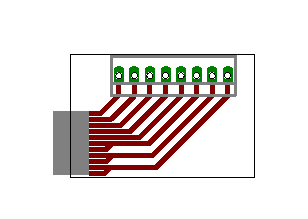
\includegraphics[width=0.5\textwidth]{figures/expansion_board.pdf}
	\caption{Left leg extension PCB schematic}
	\label{fig:pcb1}
\end{figure}

% subsubsection extension_pcbs (end)


% subsection electric_actuators (end)
%!TEX root = ../../../../report.tex

\subsection{Sensory feedback} % (fold)
\label{sub:sensory_feedback}
As stated in the initial description of the project in \ref{sec:overall_description}, the first prototype of Rubi has been designed to provide the necessary capabilities to be controlled by an existing neural controller developed in \cite{dacbot1} and already tested in the DACbot robot.
The cited control algorithm requires as inputs the angular positions of all the joints in can actuate, besides ground contact signals from the feet for its reflex-based controller part.
All the documentation regarding the handling of the sensor readings software-wise is to be found in section \ref{sec:software}.


\subsubsection{Joint position information} % (fold)
\label{ssub:joint_position_feedback}
To provide the physical readings of the angular positions of the joints, the built-in hall sensors in the motors are utilized. 
Three wires transmit the hall effect sensors signals to the motor board for each joint, where they are written in the internal register and transferred to the main processor for its posterior treatment.
% subsubsection joint_position_feedback (end)

\subsubsection{Ground contact signal} % (fold)
\label{ssub:ground_contact_feedback}
One contact switch model Omron D2F-01F-T has been placed on the edge of the sole of each foot, under the heel in order to detect when the feet are standing on the ground. 
Their wiring has been extended to the main processor board, but the necessary pull-up resistors have not been implemented since the input pins on the processor could not be set up.
The necessary mapping between the processor's GPIOS handlers and the physical pins on the board could not be found.
Therefore this last step is left as further work.
Alternatives to the use of the main board pins are discussed in chapter \ref{cha:discussion}, in case they cannot be used.
% subsubsection ground_contact_feedback (end)

% subsection sensory_feedback (end)

% section electronics (end)
%!TEX root = ../../../report.tex
\section{Mechanics} % (fold)
\label{sec:mechanics}

%!TEX root = ../../../../report.tex
\subsection{Pulleys and belts} % (fold)
\label{sub:pulleys_and_belts}
The section \ref{sec:joints} is dedicated to analyze and define what kind of motors and trasmision system is going to be used for each joint.
In the case of the knee and the ankle, the combination \textit{motor + gearbox + belt and pulleys} is chosen due to the preference of having the active actuator in the highest part of the link with the withdrawal of transfer the movement the the lowest.
This system has been design along with the torsional springs disussed in the section \ref{sub:compliance} where the rotation from the motor must feed the rotation of a serial rotational spring.
This implies the design of a system in which pulley and spring holder must be gathered.
The design of the pulley itself though, has been studied in terms of two factors: \textit{precision and backlash reduction} and \textit{integration with the serial rotational spring}.

\subsubsection{Precision and backlash reduction} % (fold)
\label{ssub:precision_and_backlash_reduction}
The goal of this design was to optimize the pulley to get a lack of backlash.
Despite the platform is going to be used mainly for self-learning controllers (e.g. based on neuronal networks) and then the mechanical optimization is not a priority, the reduction of mechanical uncertainty is always good.

After analyze all the current market several non-backlash solutions are found.
Stands out the Gates GT3 Synchronous Belts \footnote{http://www.gates.com/products/industrial/industrial-belts/synchronous-belts/powergrip-gt3-belts} that is assured to be suitable for the presented application.
The withdrawals of this design are the lack of time for ordering such parts and the increase in the final price of the product. 
However there is another important factor, the integration that must be done with the serial rotational spring.
% subsubsection precision_and_backlash_reduction (end)

\subsubsection{Integration with the serial rotational spring} % (fold)
\label{ssub:integration_with_the_serial_rotational}
Another solution is to design the pulley itself which would let to have a complete control of the design and manufacturability giving the possibility of integrate in a unique part design, the pulley for the transmission system and the spring holder.

At first, the GT3 design from Gates was intended to be designed.
However, its design is described in U.S. Patent Number 4,515,577, which doesn't allow its use.
Thus, the belts have been designed following the ISO 13050:2014 \cite{ISO13050} following the type T due to its focus in efficiency and reduction of backlash.
It is also appropriate for precision movements, high torques and low speeds, as our requirements.

The physical properties of the pulleys as the number of teeth, width, etc... have been chosen based on the ISO 5295:1987 \cite{ISO5295} and in sake of manufacturability.
As decided before, the pulley will belong to a part that will also have the task of holding the rotational serial spring.
This implies that the part will be designed to be 3D printed and thus, the criteria of design oriented to manufacturability must be applied.

Based on both ISO norms cited before and after some iterations based on experimental tests the pulley T2,5 of 19 teeth gave the expected behavior.
Both pulleys are the same so no reduction is given from the motor shaft to he other.
In the figure \ref{fig:motor_pulley}, a detail of the designed pulleys can be seen.
% subsubsection integration_with_the_serial_rotational (end)

% subsection pulleys_and_belts (end)
%!TEX root = ../../../../report.tex
\subsection{Gears} % (fold)
\label{sub:gears}

% subsection gears (end)
%!TEX root = ../../../../report.tex
\subsection{Impact force} % (fold)
\label{sub:impact_force}
In order to calculate the physical dimensions of some of the components, a bounding conditions have to be defined.
The presented case shows a peak of energy when landing after being jumped a estimated height.
This energy in then transmitted from the first contact point, the footprint, to the rest of the system, causing efforts that must be absorbed.
The components of the system must receive that energy under a controlled behavior -this is elastic deformations- assuring a longer life cycle of the legs.

Thus, some input parameters to calculate the impact force are assumed.
From this force will be sized all the consecutive components in the deformation chain.
Despite the deformation is of the whole system, the security coefficient assumed in here is going to be the calculation of all the components for that maximum force.

From the formula of the mechanical energy:
\begin{equation}
  E_{mechanical} = m g \Delta h + \frac{1}{2} m v^{2}
\end{equation}

The kinetic energy is negligible and only the energy form falling a certain height is supposed.
This energy is then translated into force by supposing a deformation of the whole body:
\begin{equation}
\label{eq:impact_force}
  F_{impact} = \frac{m g \Delta h}{t_{impact\_displacement}}
\end{equation}

The equation \ref{eq:impact_force} gives the force for sizing all the components.
Based on the input parameters defined in the appendix \ref{app:profile_selection} which are:
\begin{table}
\begin{center}
\begin{tabular}{c | c}
  Parameter & Value \\
  \hline
  Total mass [kg] & 1.5 \\
  Jumping height [m] & 0.1 \\
  Impact displacement [m] & 0.005
\end{tabular}
\caption{Input parameters for calculating the impact force}
\label{tab:input_parameter_impact_force}
\end{center}
\end{table}

The impact force is then:
\begin{equation}
  F_{impact} = \frac{m g \Delta h}{d_{impact\_displacement}} = 294.40 N 
\end{equation}
% subsection impact_force (end)
%!TEX root = ../../../../report.tex
\subsection{Limb profile} % (fold)
\label{sub:limb_profile}
Based on the requirements of weight and its distribution defined in the analysis of the joints \ref{sec:joints}, the links have been decided to have in the upper extreme the actuators. 
This leads to use a transmission system, such as belt and pulleys, which leaves for the rest of link a structural function that can also adopt the task of wiring placement.
Thus, a light weight section that satisfy the conditions of deformation and stress maximum will be chosen.
Carbon fiber is an ideal material to achieve this conditions of weight and stress so an quantitative analysis has been made calculating the optimal solution and then rounding it for all the possible profiles offered by the given provider.
The provider was chosen due to the previous experiences that the Mærsk Mc-Kinney Møller Institute had with carbon fiber orders.

The section profile offered \footnote{http://www.easycomposites.co.uk/\#!/cured-carbon-fibre-products/} are: \textit{Rod}, \textit{Tube}, \textit{Box}. The \textit{Stripe} and the \textit{Angle} are discarded due to its asymmetrical geometry that will will lead to less predictable scenarios.
The study case is show in the figure \ref{fig:impact_decomposition}, where the impact force can be decomposed in a pure bending effort and a pure compression.
Due to the resistance of the carbon fiber in pure compression is bigger than in bending, only this last case has been studied.
This studies should not completly follow the behaviour in real life due to the carbon fiber is not an isomorphic material.
However, the high security factor taken into account is expected to overcome this assumption.

\begin{figure}[ht!]
  \centering
  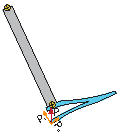
\includegraphics[width=.3\textwidth]{figures/impact_decomposition.pdf}
  \caption{Impact force decomposed}
  \label{fig:impact_decomposition}
\end{figure}

\subsubsection{Profile study} % (fold)
\label{ssub:profile_study}
  The bending effort causes two sort of problems: (1) the possible break in the supporting point and (2) the deformation suffered by the beam.
  The break will occur when the tensions created will be over the ultimate tension in compression or tension of the selected material.
  This comes defined in the equation \ref{eq:tension} for symmetric sections and when an only torque is being applied.
  \begin{equation}
  \label{eq:tension}
    \sigma _{compression} = \sigma _{tension} = \frac{M h_{CG}}{I_x}
  \end{equation}

  Meanwhile the deformation in the extreme can be calculated with the equation \ref{eq:deformation} if the case is simplified to the occurred in the figure \ref{fig:impact_decomposition}.
  This is, when the legs is completely stretched, what will cause the biggest stresses.

  \begin{figure}[ht!]
    \centering
    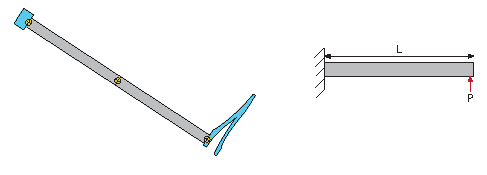
\includegraphics[width=\textwidth]{figures/bending_case.pdf}
    \caption{Simplified representation of the bending case}
    \label{fig:bending case}
  \end{figure}

  \begin{equation}
  \label{eq:deformation}
    y_L = \frac{P z^2}{6EI}(3L-z) = \frac{P L^2}{6EI}(2L) = \frac{P L^2}{3EI}
  \end{equation}


  For the selected profiles the equations that define the compression $\sigma _{compression}$ and tension efforts $\sigma _{tension}$, along with the deformation in the direcction of the applied force $y_L$ are shown, being:

  \begin{enumerate}
    \item $h_{CG}$: height of the center of gravity of the semi-half section from the geometrical center of the section.

    \item $E$: Elastic module.
  \end{enumerate}


  \noindent\begin{minipage}{0.2\textwidth}% adapt widths of minipages to your needs
      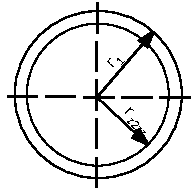
\includegraphics[width=\linewidth]{figures/profile_cylinder.pdf}
  \end{minipage}%
  \hfill%
  \begin{minipage}{0.8\textwidth}
    \begin{equation}
      \begin{aligned}
      \sigma _{compression} = \sigma _{tension} &= \frac{M h_{CG}}{I_x} = \frac{4 r_2}{\pi(r_2 ^4 - r_1 ^4)} M \\
      y_L &= \frac{P L^2}{3EI} = \frac{4 P L^2}{3 E \pi(r_2 ^4 - r_1 ^4)}\\
      h_{CG} &= r_2 \\
      I_x = I_y &= \frac{\pi}{4} (r_2 ^4 - r_1 ^4)
      \end{aligned}
    \end{equation}
  \end{minipage}

  \noindent\begin{minipage}{0.2\textwidth}% adapt widths of minipages to your needs
      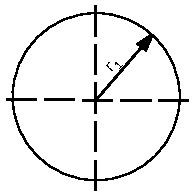
\includegraphics[width=\linewidth]{figures/profile_tube.pdf}
  \end{minipage}%
  \hfill%
  \begin{minipage}{0.8\textwidth}
    \begin{equation}
    \begin{aligned}
      \sigma _{compression} = \sigma _{tension} &= \frac{M h_{CG}}{I_x} = \frac{4}{\pi r_1 ^3} M\\
      y_L &= \frac{P L^2}{3EI} = \frac{4 P L^2}{3 E \pi r_1 ^4}\\
      h_{CG} &= r_1 \\
      I_x = I_y &= \frac{\pi r_1 ^4}{4}
      \end{aligned}
    \end{equation}
  \end{minipage}

  \noindent\begin{minipage}{0.2\textwidth}% adapt widths of minipages to your needs
      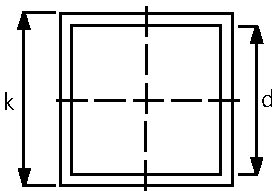
\includegraphics[width=\linewidth]{figures/profile_squared.pdf}
  \end{minipage}%
  \hfill%
  \begin{minipage}{0.8\textwidth}
    \begin{equation}
    \begin{aligned}
      \sigma _{compression} = \sigma _{tension} &= \frac{M h_{CG}}{I_x} = \frac{6 d}{(d^4 - k^4)}\\
      h_{CG} &= \frac{d}{2} \\
      y_L &= \frac{P L^2}{3EI} = \frac{4 P L^2}{E (d^4 - k^4)}\\
      I_x = I_y &= \frac{1}{12} (d^4 - k^4)
      \end{aligned}
    \end{equation}
  \end{minipage}
% subsubsection profile_study (end)

\subsubsection{Torque calculation} % (fold)
\label{ssub:torque_calculation}
  For both cases, the profile of the lower limb and the upper, the torque generated by the impact force determined in the section \ref{sub:impact_force}, is calculated.
  This torque is different in the lower and the upper limb due to the upper limb takes the distance from the foot to the hip while the other one is only from the foot to the knee:
  \begin{equation}
  \begin{aligned}
     M_{lower\ limb} = F \cdot d = 294.4 \cdot 0.2126 = 62.57 Nm\\
     M_{upper\ limb} = F \cdot d = 294.4 \cdot (0.2126 + 0.2622) = 139.73 Nm
  \end{aligned}
  \end{equation}
% subsubsection torque_calculation (end)

\subsubsection{Final limb parameters} % (fold)
\label{ssub:final_limb_parameters}
Following the criteria from the sections \ref{sec:dimensions} and \ref{sec:physical_properties} of size and materials, the presented formulas and the have been applied to all the profiles of the provider.
An iterative processes based on the outputs of the mathematical model \ref{cha:mathematical_model} has given a result the limb lengths shown in the table \ref{tab:limb_lengths}.

\begin{table}[ht!]
\centering
\caption{Final limb lengths}
\label{tab:limb_lengths}
\begin{tabular}{r|l}
  \textbf{Limb} & \textbf{Length [m]} \\ \hline
  Foot & 0.095 \\ \hline
  Lower limb & 0.212 \\ \hline
  Upper limb & 0.262    
\end{tabular}
\end{table}

\todo{Add hip and foot width with small explanation}

Then, the profiles have been analyzed calculating the torque from \ref{ssub:torque_calculation} and then applying the section \ref{ssub:profile_study} for each iteration.
The calculations of the last iteration are shown in the appendix \ref{app:profile_selection}.
These results have been then approved or discarded based on a \textit{maximum deformation} and \textit{ultimate tension} requirements, and are shown in the table \ref{tab:profile_selection}

\begin{table}[ht!]
\centering
\caption{Profile selection for each limb}
\label{tab:profile_selection}
\begin{tabular}{c|c|c}
  \textbf{Limb} & \textbf{Section} & \textbf{Dimensions} \\ \hline
  Lower limb & Tube & 20 mm and 1 mm thickness \\ \hline
  Upper limb & Tube & 20 mm and 1 mm thickness 
\end{tabular}
\end{table}

% subsubsection profile_selection (end)



% subsection limb_profile (end) 
%!TEX root = ../../../../report.tex

\subsection{Bearings} % (fold)
\label{sub:bearings}
In the section \ref{sub:impact_force} the force for sizing the bearings of the knee and the ankle was calculated.
The bearing elected would be such that allows dynamic loads of more than the impact force while keeping as small as possible to reduce the added weight to the robot.
On the other hand, the internal diameter comes defined by the rod diameter calculated in the section \ref{sub:rods}.

An estimation of nominal life of the bearing can be done from the Dynamic Load Rating (C), the Dynamic Equivalent Load (P) and the Life Rime Coefficient for a Ball Bearing (p) (being p=3 for balls bearings).
The equation \ref{eq:service_life_bearing}, shows the nominal life of a ball bearing that can be used in order to calculate the nominal life for a specific application.
It is also worth to mention that the Dynamic Equivalent Load (P) is divided by the number of bearings in which the force is spread.
\begin{equation}
  \label{eq:service_life_bearing}
  L_{10} = \frac{10^{6}}{60 n} \left(\frac{C}{P}\right)^{p}
\end{equation}

The term $L$ is the service life of a bearing (in number of hours or rpm), in normal conditions of speed and load, in which the bearing is working until fail by fatigue. 
Whilst $L_{10}$ is based in a stadistical model that is defined as the 90\% of the bearing of the same type will withstand those loads for a longer time.
% subsection bearings (end)
%!TEX root = ../../../../report.tex
\subsection{Rods} % (fold)
\label{sub:rods}
As explained in section \ref{sub:bearings}, was decided to have two bearings per link (which gives four per joint) and a rod going through them.
This rod is then also used, in the case of the knee and the ankle, as a support for the pulleys that transmit the power from the pulley to the next link.

Three mechanical efforts bound its design:
\begin{enumerate}
  \item \textbf{Shear strenth}: in the case of the shear produced when an impact occurs and the rod of one link moves in the opposite direcction than its relative in the consecutive link.
  \item \textbf{Resistance to beding}: due to the bending effort that the tension of the belt is constantly applying in the rod of the  knee and the ankle.
  \item \textbf{Torsion}: due to the pulley in the knee and the ankle. 
  This effort is negligible because zero-friction bearings are supposed.
\end{enumerate}

  \subsubsection{Shear analysis} % (fold)
  \label{ssub:shear_analysis}
  The maximum shear stress is found in the diameter of the cylinder (y=0) and is:
  
  \noindent\begin{minipage}{0.2\textwidth}% adapt widths of minipages to your needs
  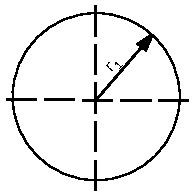
\includegraphics[width=\linewidth]{figures/profile_tube.pdf}
  \end{minipage}%
  \hfill%
  \begin{minipage}{0.8\textwidth}
    \begin{equation}
    \begin{aligned}
      \gamma_{yz} &= \frac{Q_y M_{x}^A*}{b(y) I_x} = \frac{Q}{r^2}\\
      M_{x}^{A_{y=0}} &= \frac{\pi r_1^2}{2} \\
      b(y=0) &= 2 r_1 \\
      I_x &= \frac{\pi r_1^4}{4}
      \end{aligned}
    \end{equation}
  \end{minipage}
  Given a tangent force Q, the shear stress can be calculated.
  If this is over the ultimate strength, the cylinder will break.
  % subsubsection shear_analysis (end)

  \subsubsection{Bending} % (fold)
  \label{ssub:bending}
  The beding analisys follows the one carried out in the section \ref{ssub:profile_study} for a cylinder.
  The equivalent force in this case is given by the tension of the belts, mainly the initial (thought there are other tensions that appear when the belts moves).
  Due to feasibility reasons an the lack of measurements units, some experimental tests trying differnt tensions and axis where carried out giving good results with a 3 mm rod or more.
  % subsubsection bending (end)

  \subsubsection{Sizing} % (fold)
  \label{ssub:sizing}
  The studies above have been tested for different diameters of rod starting from the smallest size given by the provider and increasing until both conditions are satisfied, due to the requirements of low weight.
  In case of using steel as material, the ultimate strength is supposed to be 250 MPa \footnote{https://en.wikipedia.org/wiki/A36\_steel}.
  And for the case of a rod of 3 mm of diameter, both stresses are under the restrictions.
  Thus, 3 mm rods are going to be used.
  % subsubsection sizing (end)
% section rods (end)
%!TEX root = ../../../../report.tex

\subsection{Finite Element Method (FEM)} % (fold)
\label{sub:finite_element_method}

% subsection finite_element_method (end)
%!TEX root = ../../../../report.tex
\subsection{Computer-Aided Design (CAD)} % (fold)
\label{sub:computer_aided_design}

\begin{figure}[ht!]
    \centering
    \begin{subfigure}[b]{0.49\textwidth}
        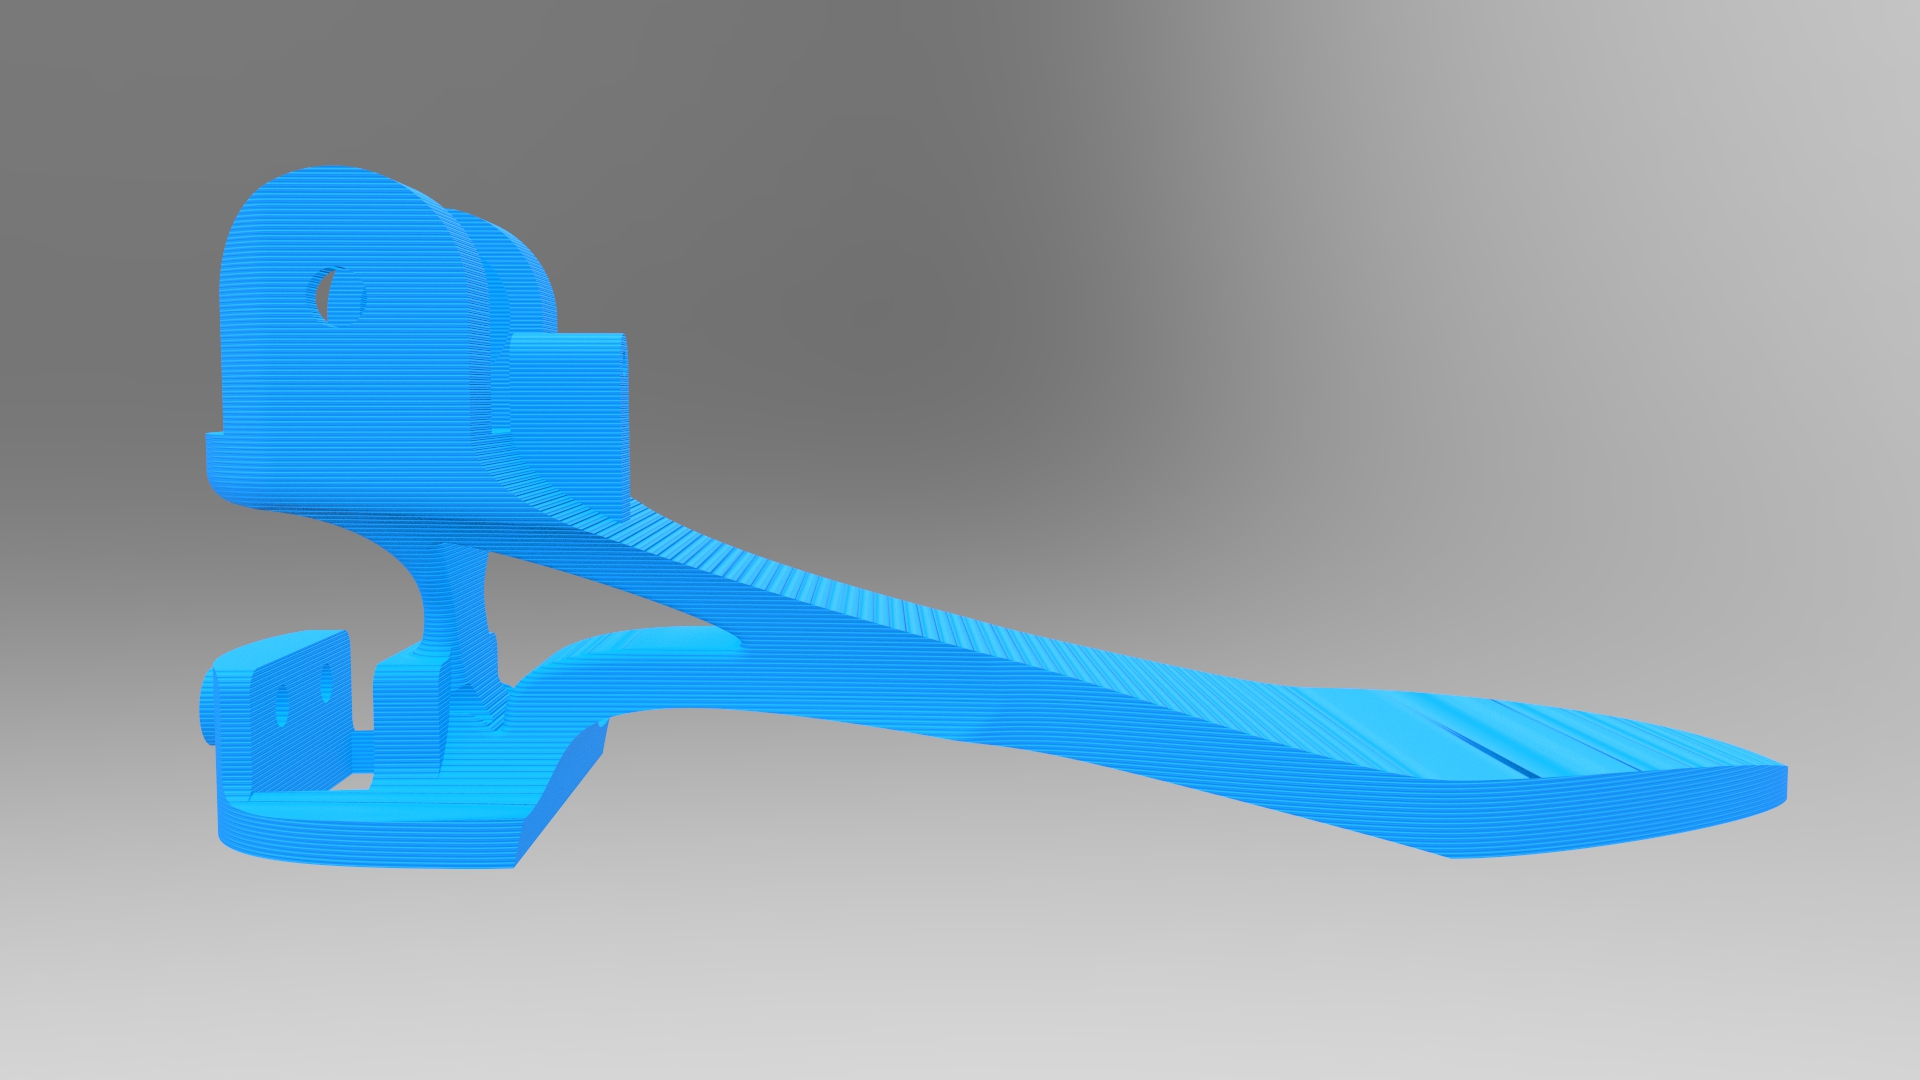
\includegraphics[width=\textwidth]{figures/legs_foot.jpg}
        \caption{Left foot}
        \label{fig:left_foot}
    \end{subfigure}
    \begin{subfigure}[b]{0.49\textwidth}
        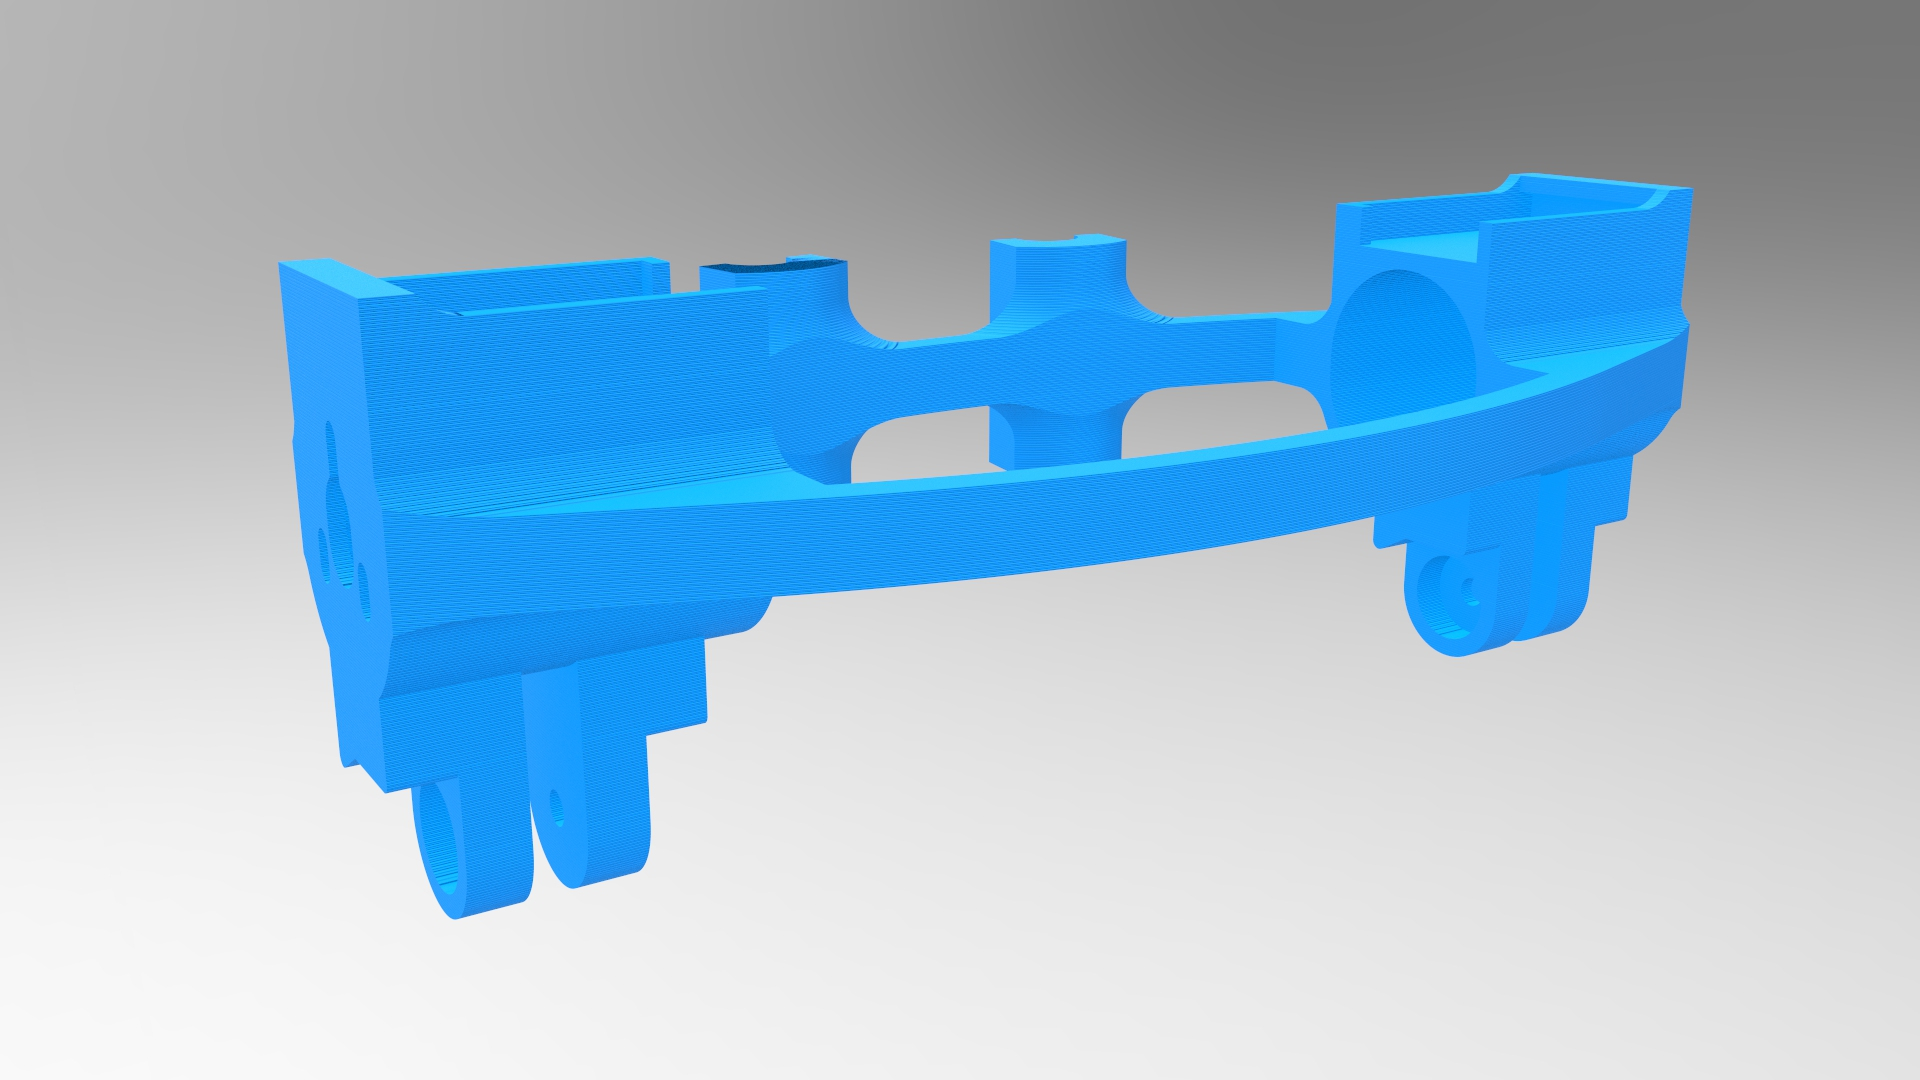
\includegraphics[width=\textwidth]{figures/legs_hip.jpg}
        \caption{Hip}
        \label{fig:hip}
    \end{subfigure}

    \begin{subfigure}[b]{0.49\textwidth}
        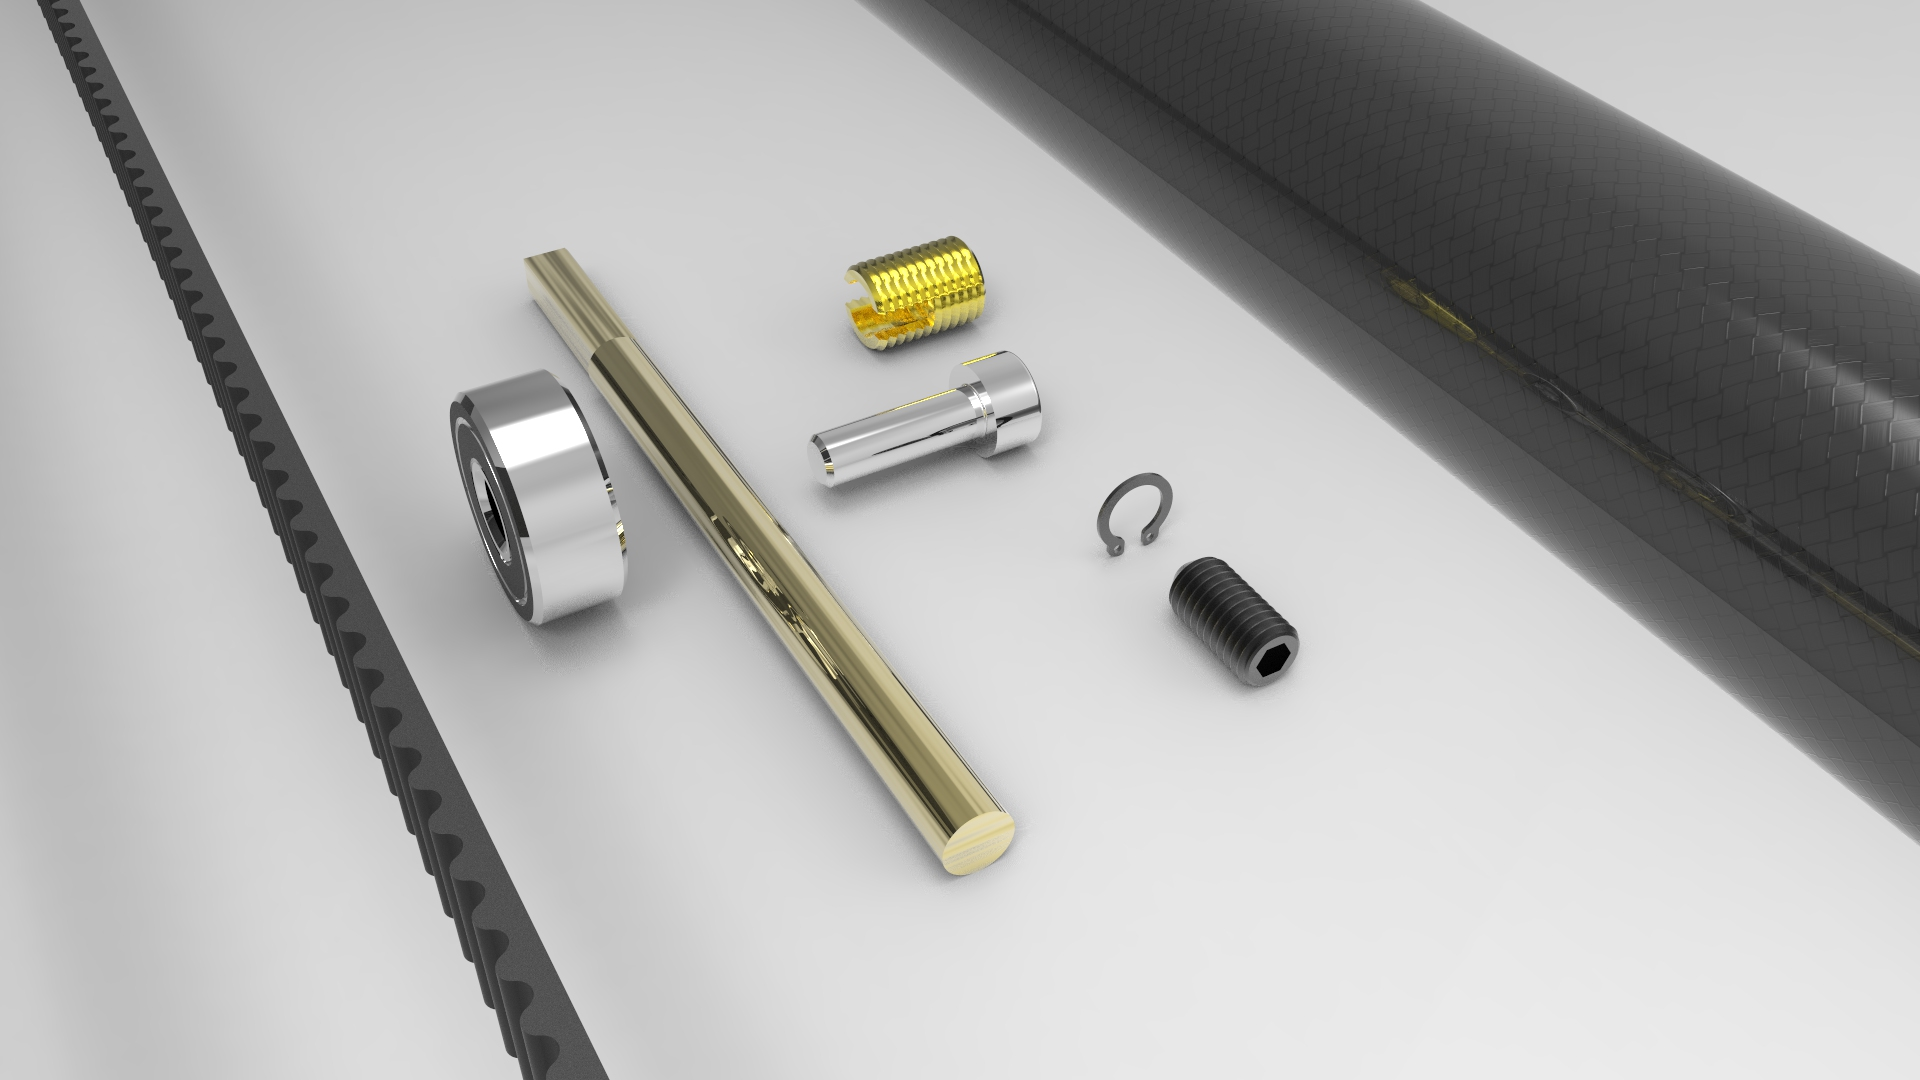
\includegraphics[width=\textwidth]{figures/legs_parts.jpg}
        \caption{Additional designed parts}
        \label{fig:mouse}
    \end{subfigure}
    \begin{subfigure}[b]{0.49\textwidth}
        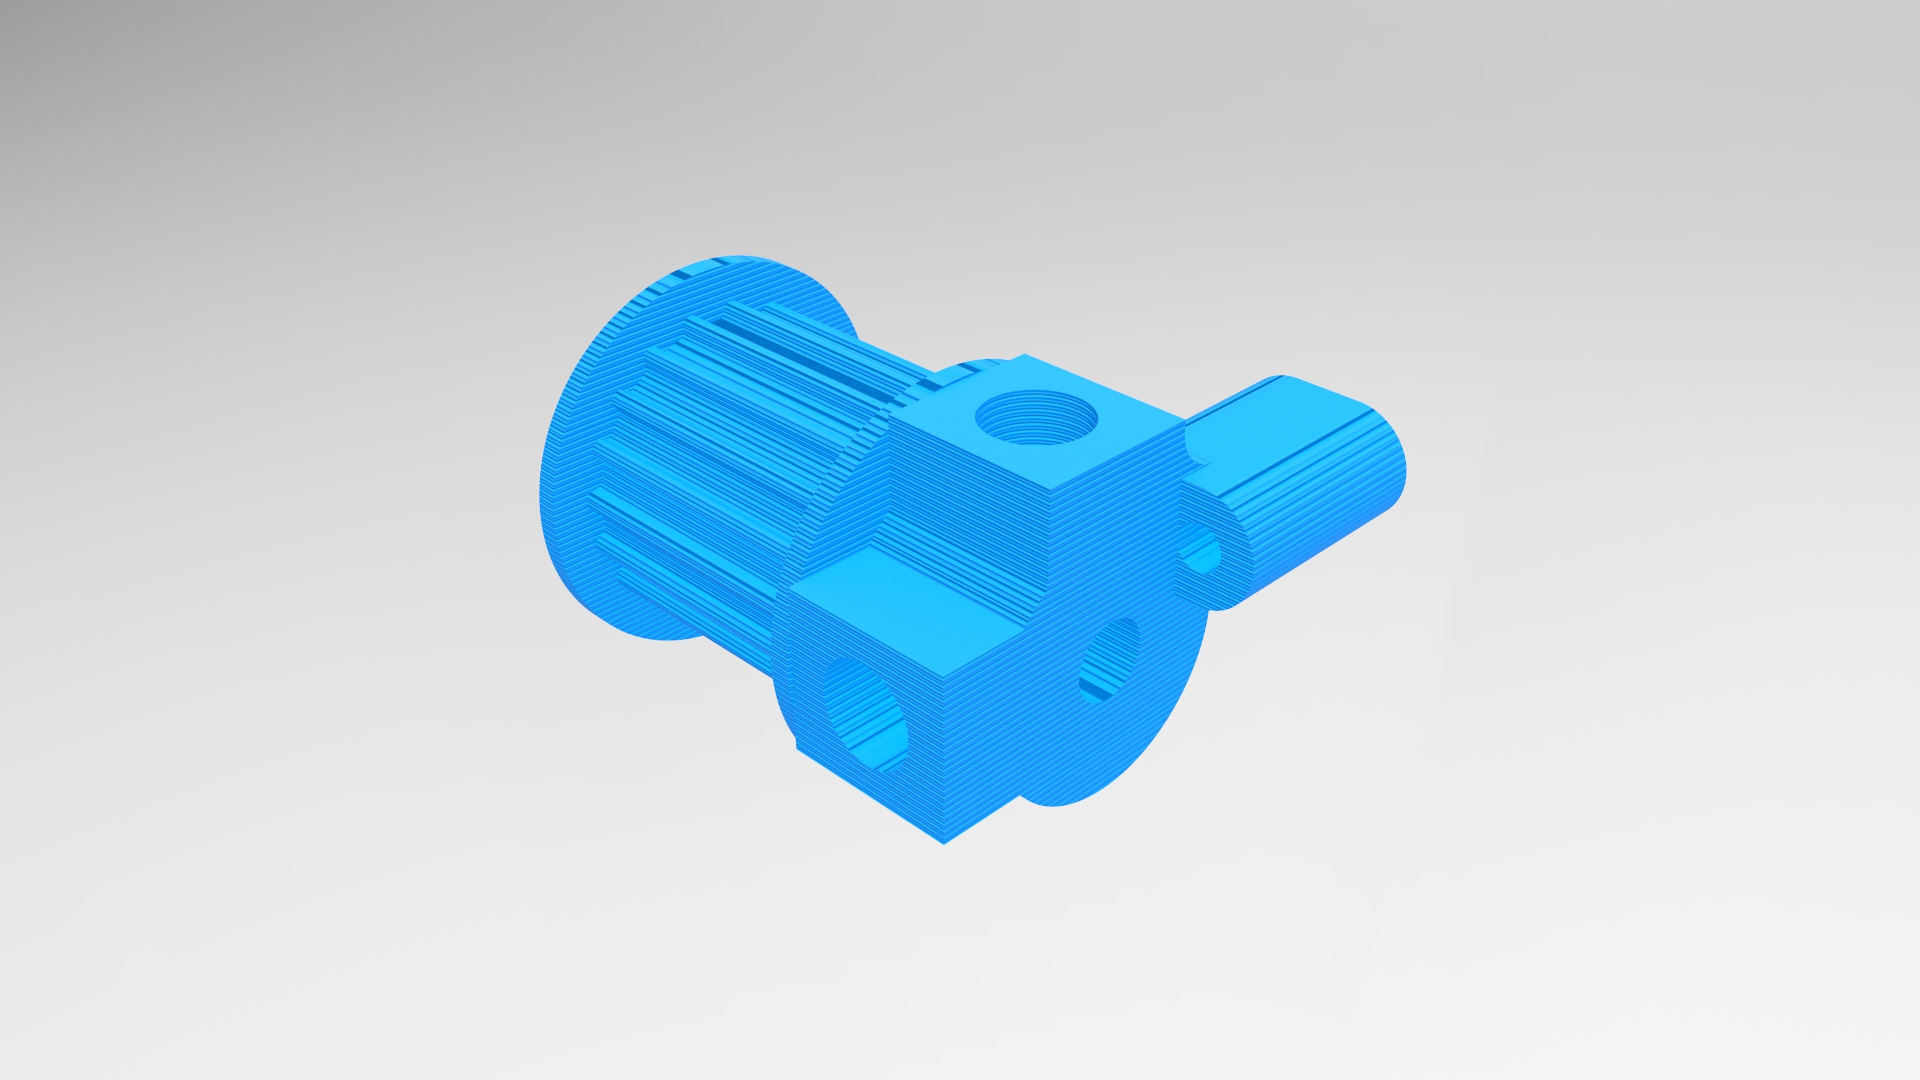
\includegraphics[width=\textwidth]{figures/legs_pulley.jpg}
        \caption{Left ankle serial spring pulley}
        \label{fig:serial_spring_pulley}
    \end{subfigure}

    \begin{subfigure}[b]{0.49\textwidth}
        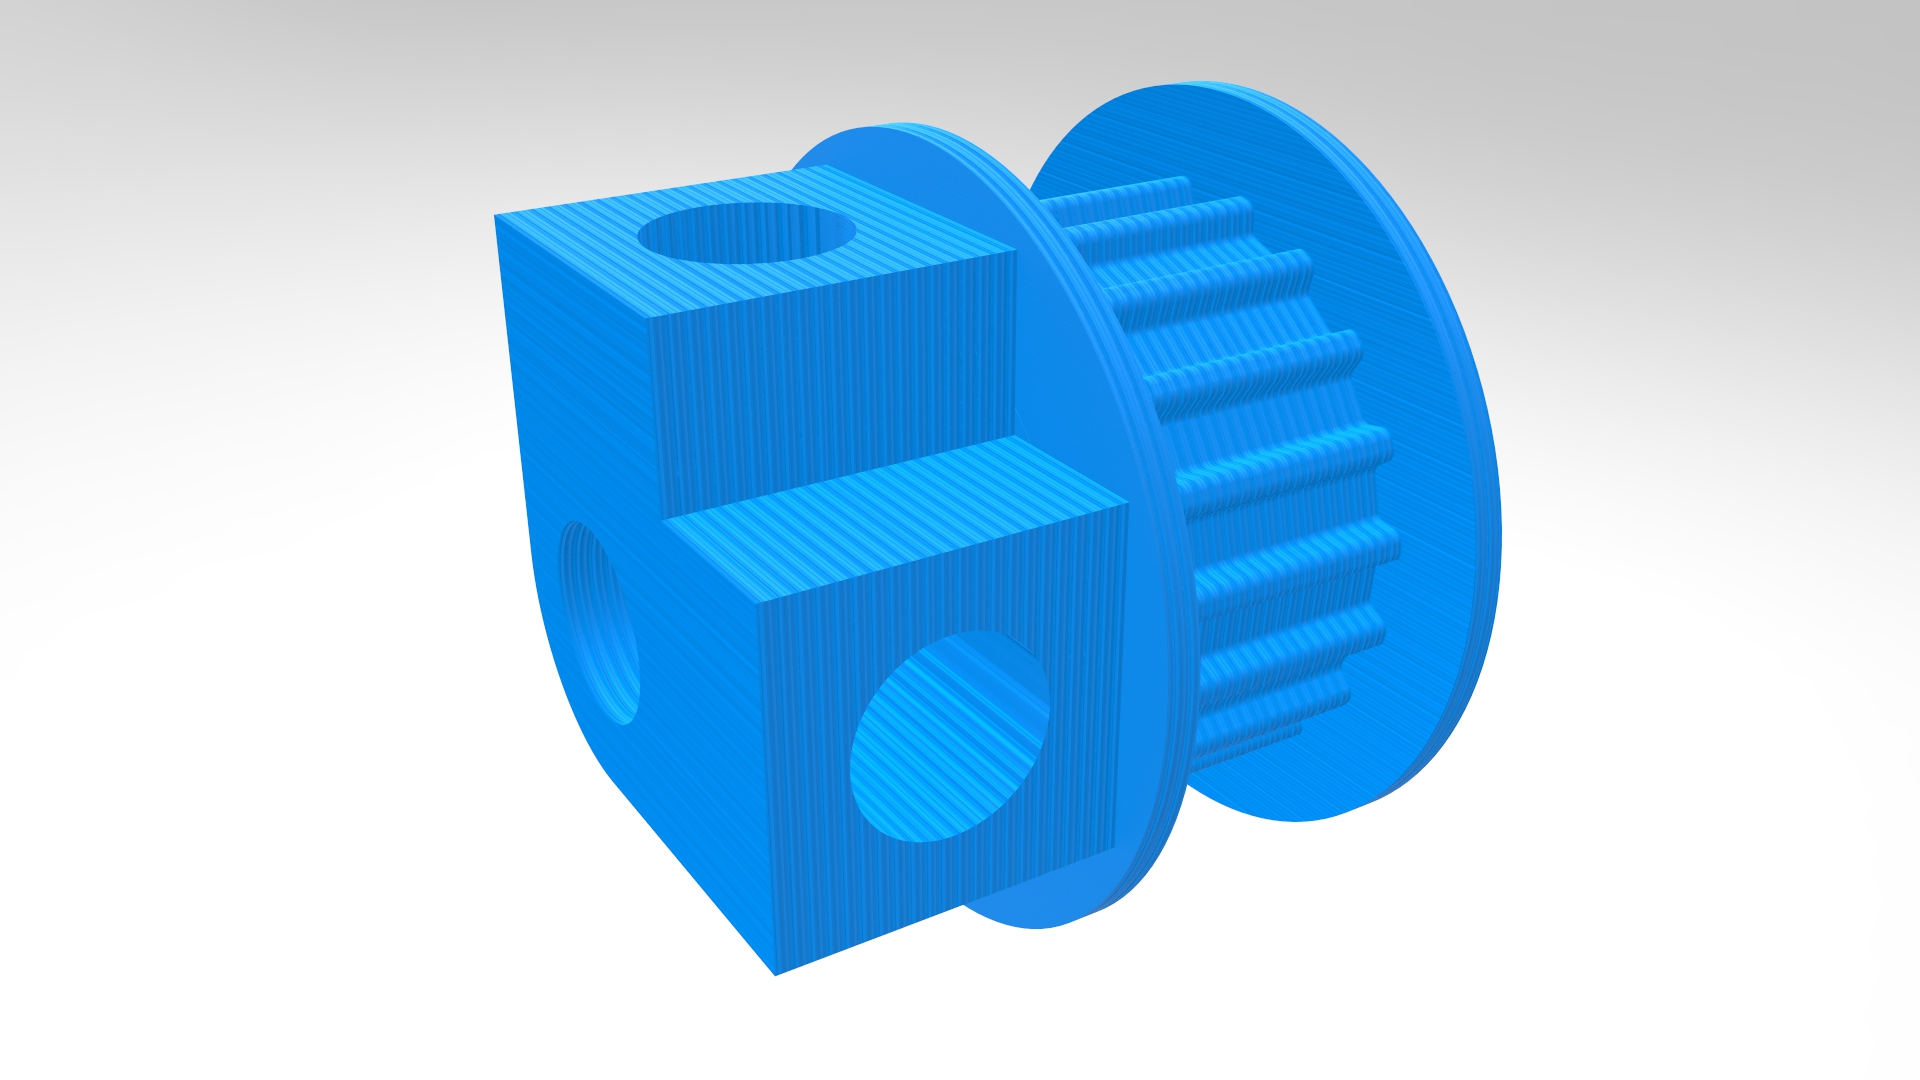
\includegraphics[width=\textwidth]{figures/legs_pulley_motor.jpg}
        \caption{Motor pulley}
        \label{fig:motor_pulley}
    \end{subfigure}
    \begin{subfigure}[b]{0.49\textwidth}
        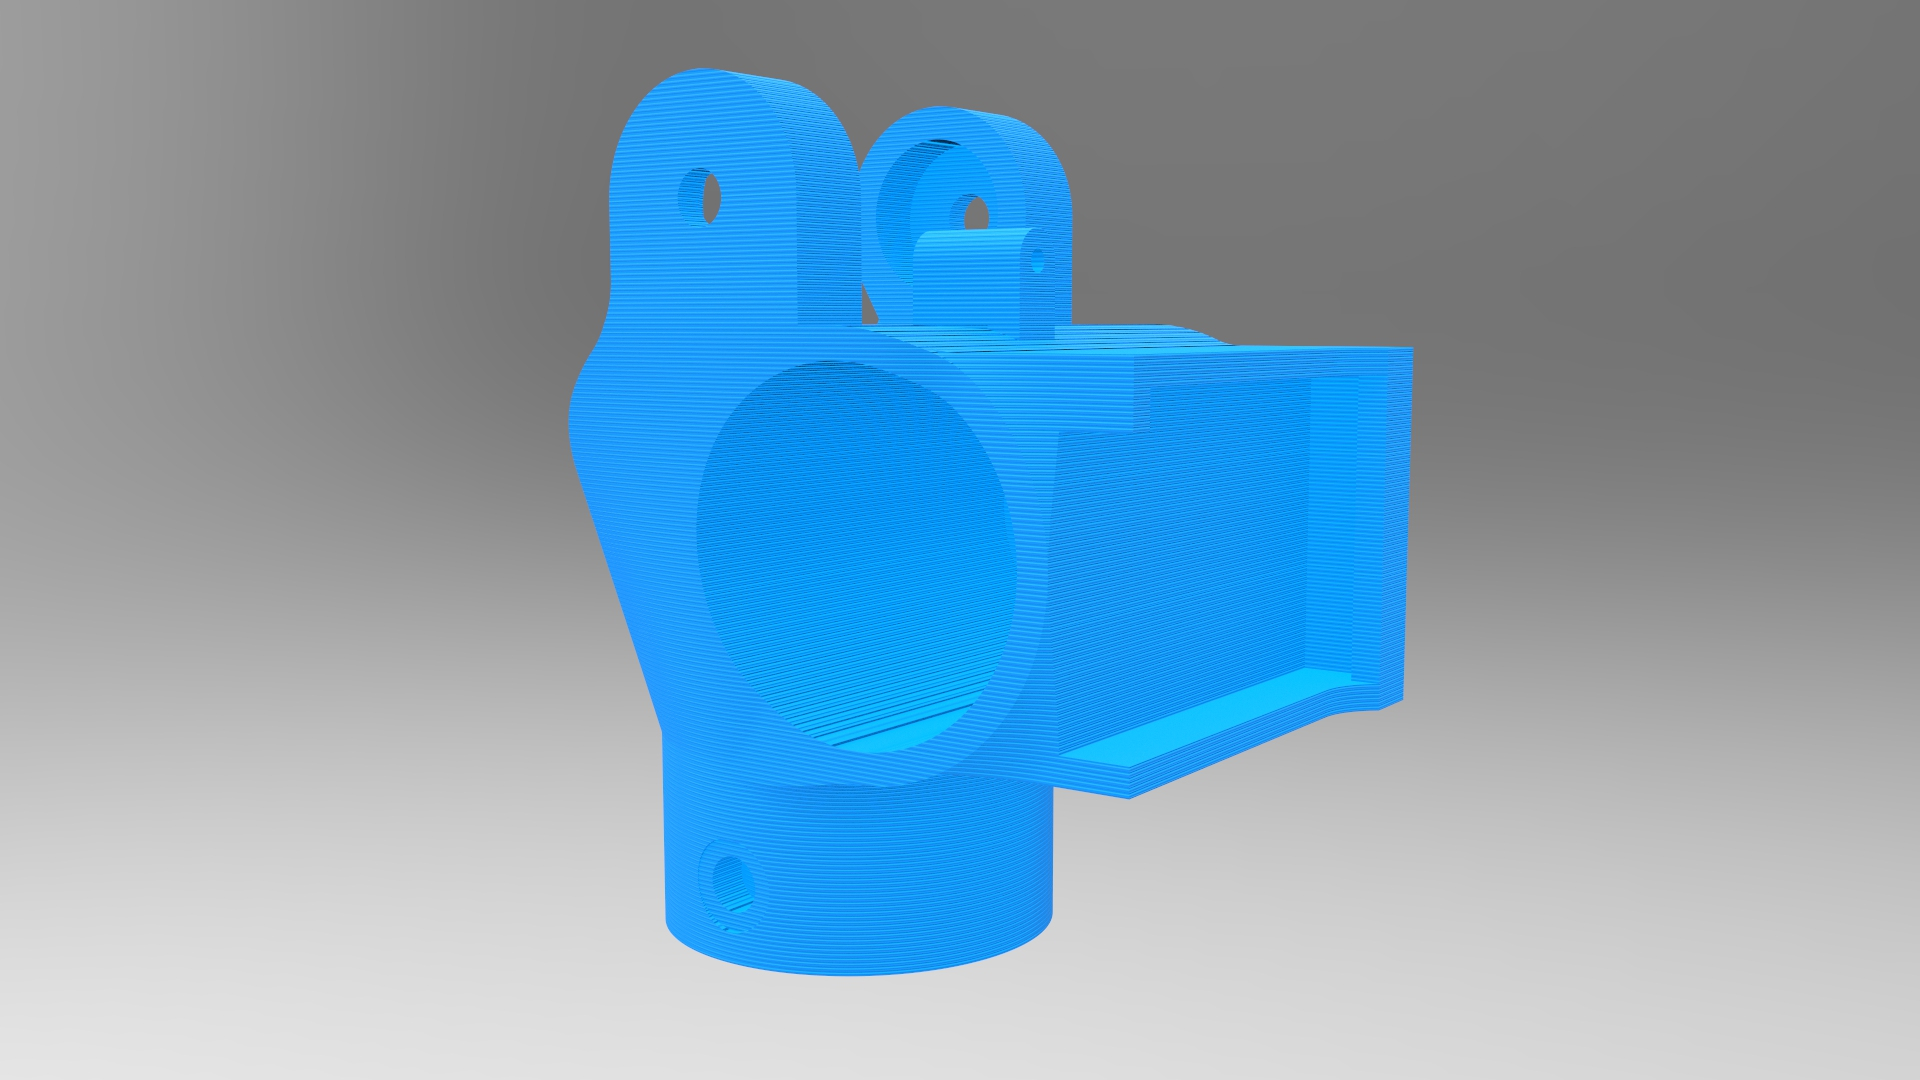
\includegraphics[width=\textwidth]{figures/legs_knee_lower.jpg}
        \caption{Left lower knee}
        \label{fig:lower_knee}
    \end{subfigure}

    \begin{subfigure}[b]{0.49\textwidth}
        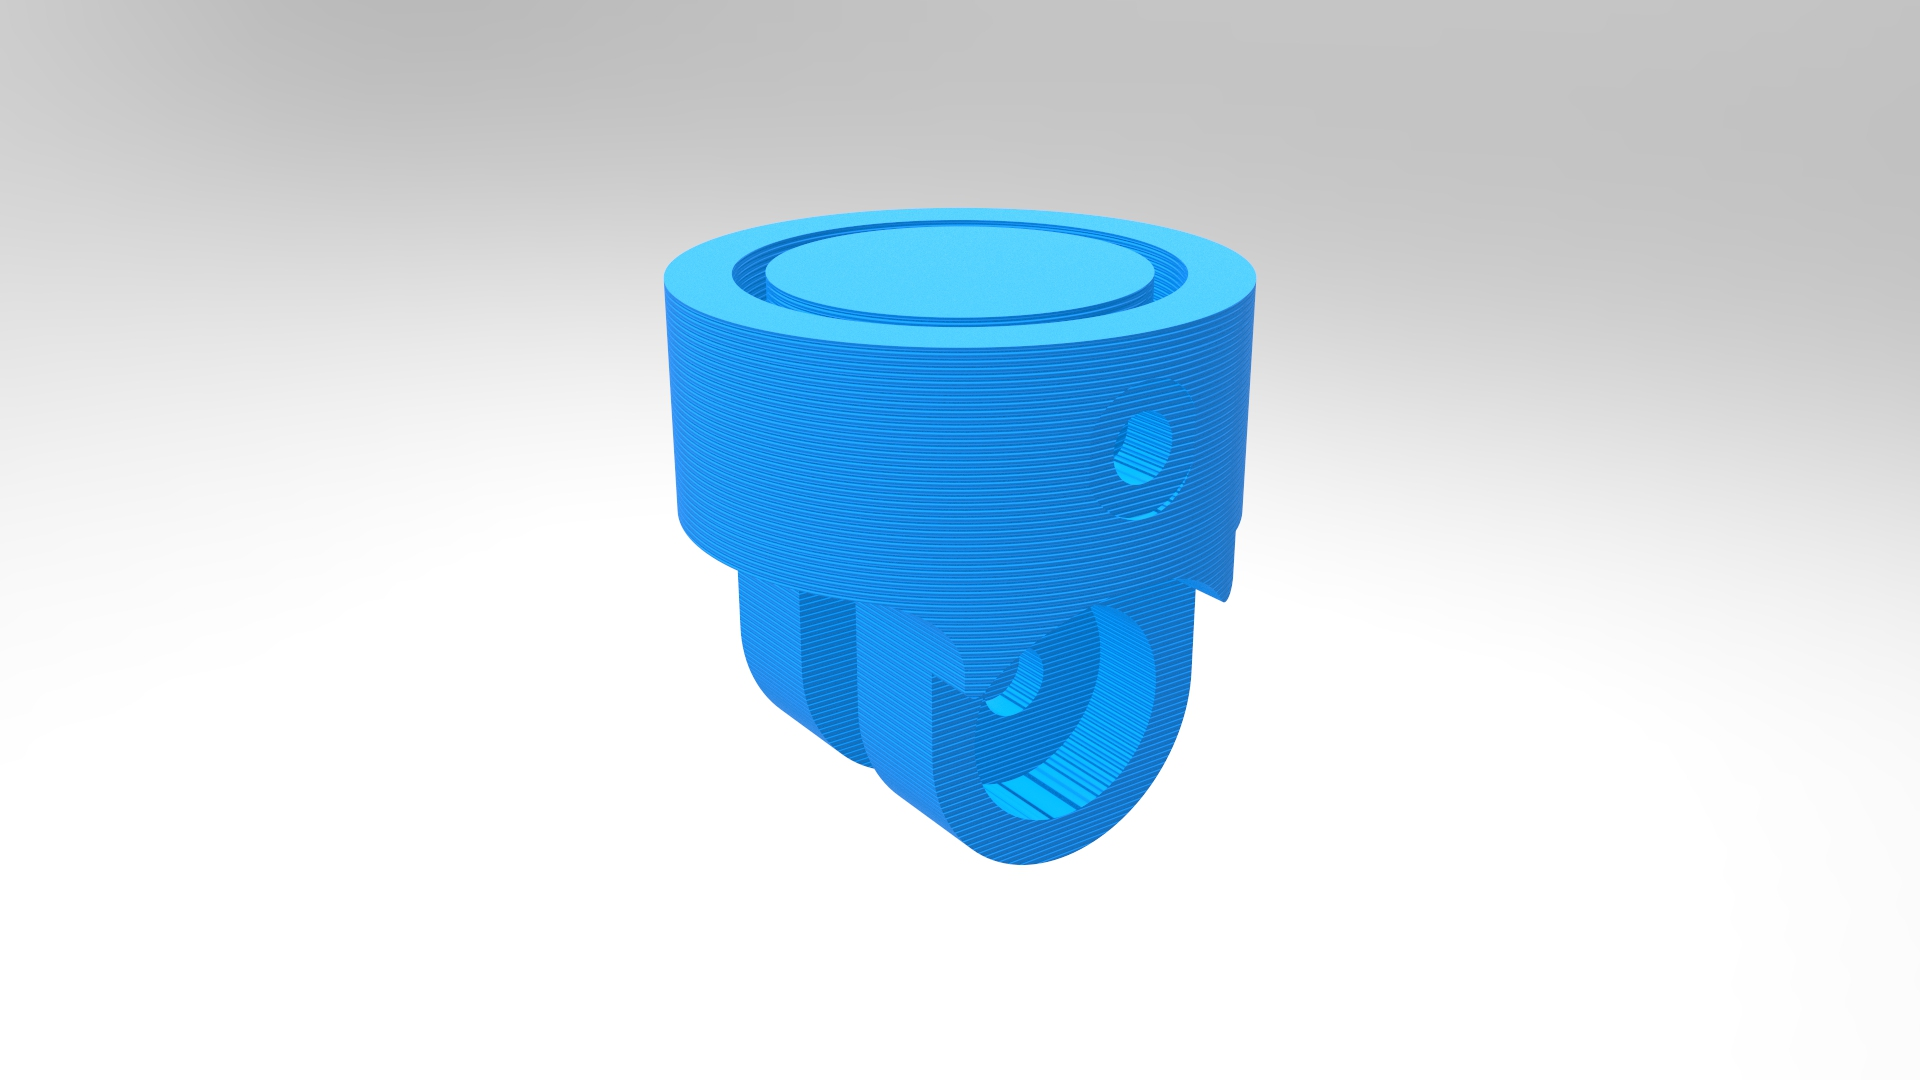
\includegraphics[width=\textwidth]{figures/legs_ankle_upper.jpg}
        \caption{Left upper ankle}
        \label{fig:ankle_upper}
    \end{subfigure}
    \begin{subfigure}[b]{0.49\textwidth}
        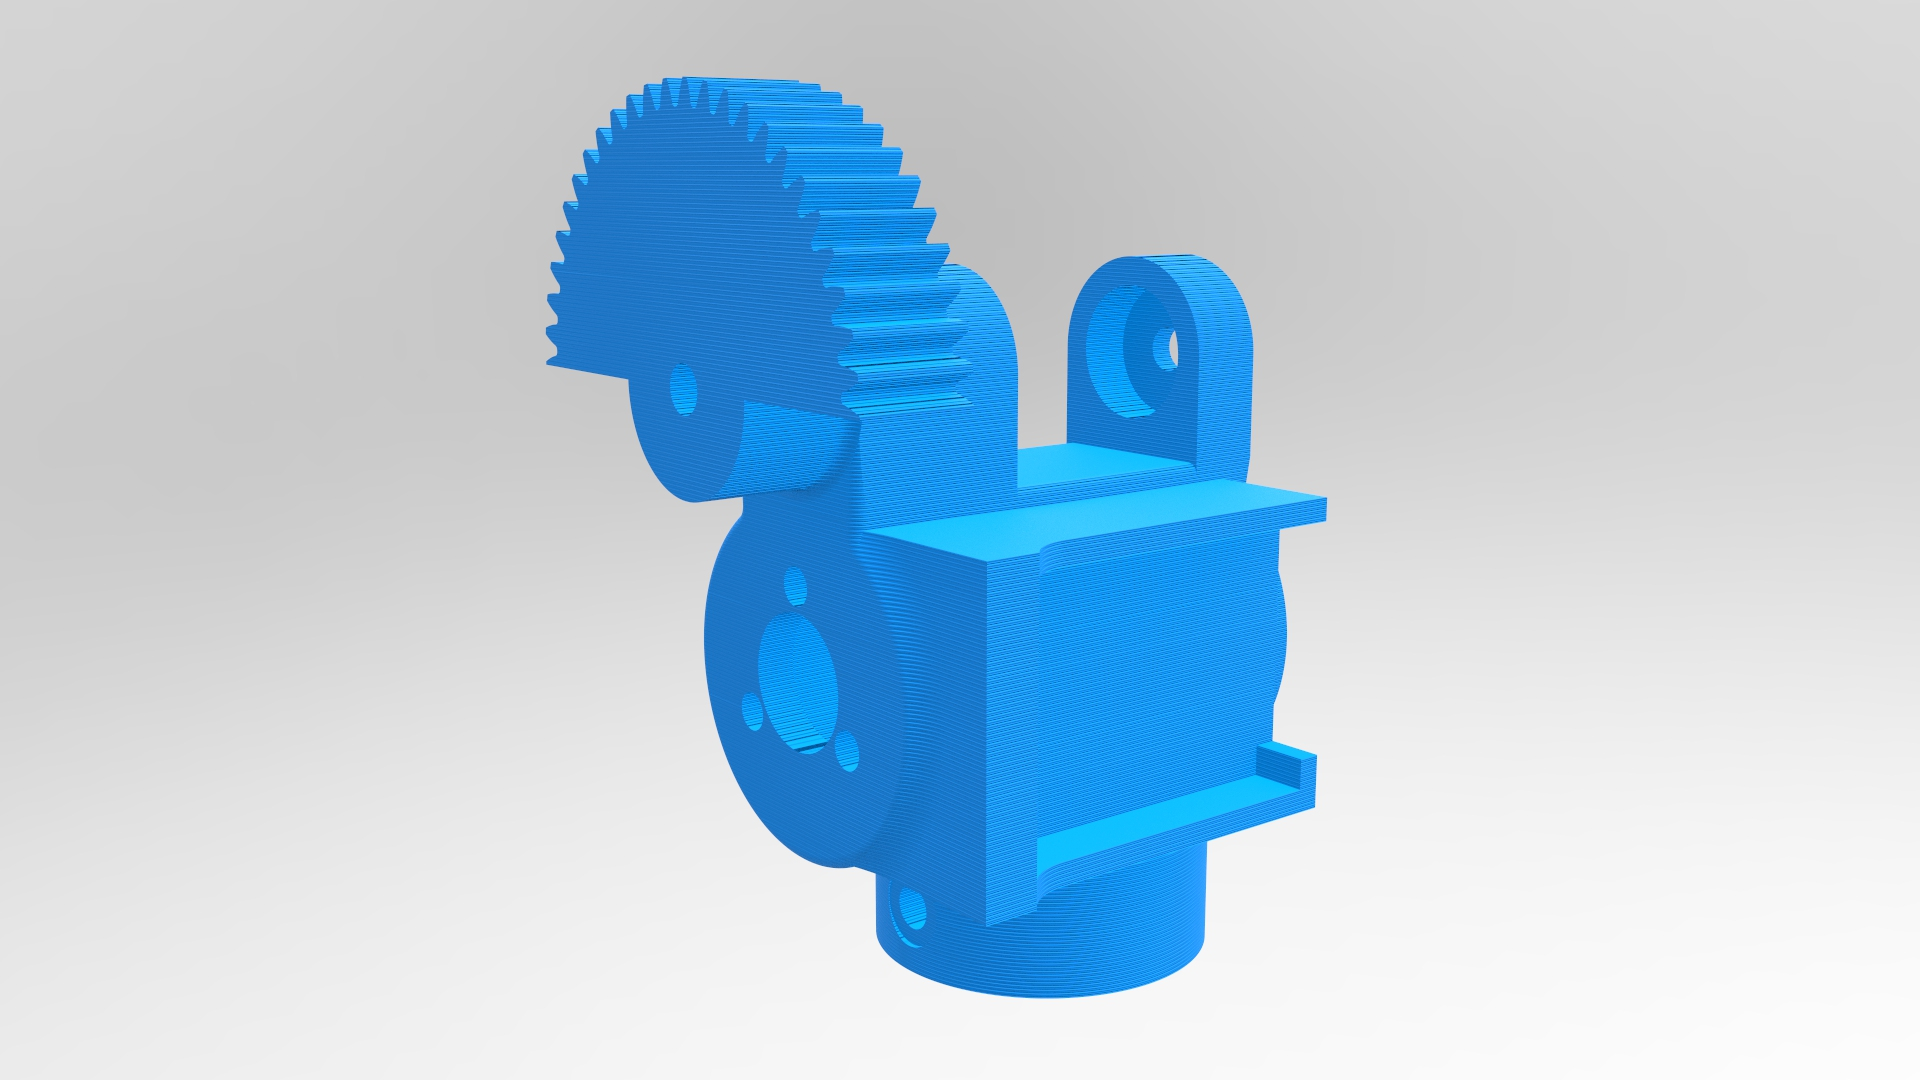
\includegraphics[width=\textwidth]{figures/legs_hip_lower.jpg}
        \caption{Left lower hip}
        \label{fig:hip_lower}
    \end{subfigure}

    \begin{subfigure}[b]{0.49\textwidth}
        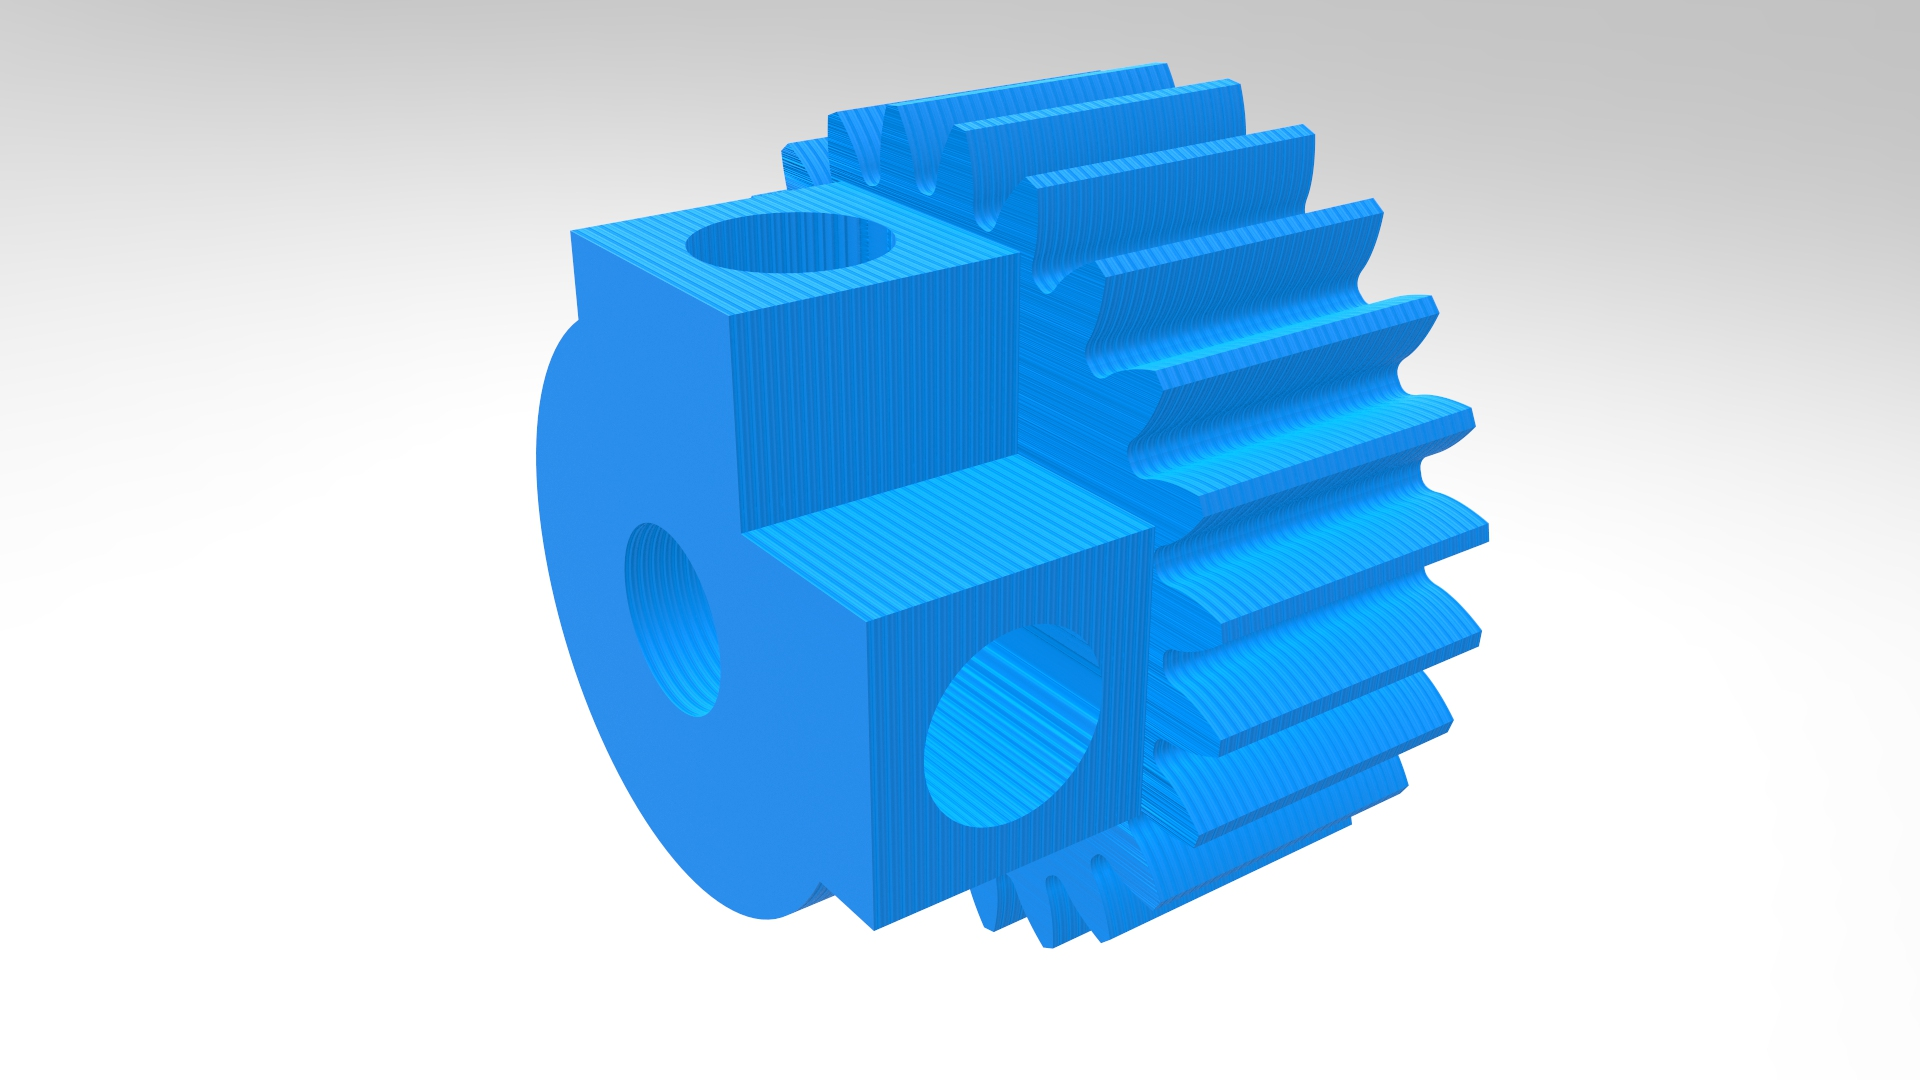
\includegraphics[width=\textwidth]{figures/legs_hip_pinion.jpg}
        \caption{Hip's pinion}
        \label{fig:hip_pinion}
    \end{subfigure}
    \begin{subfigure}[b]{0.49\textwidth}
        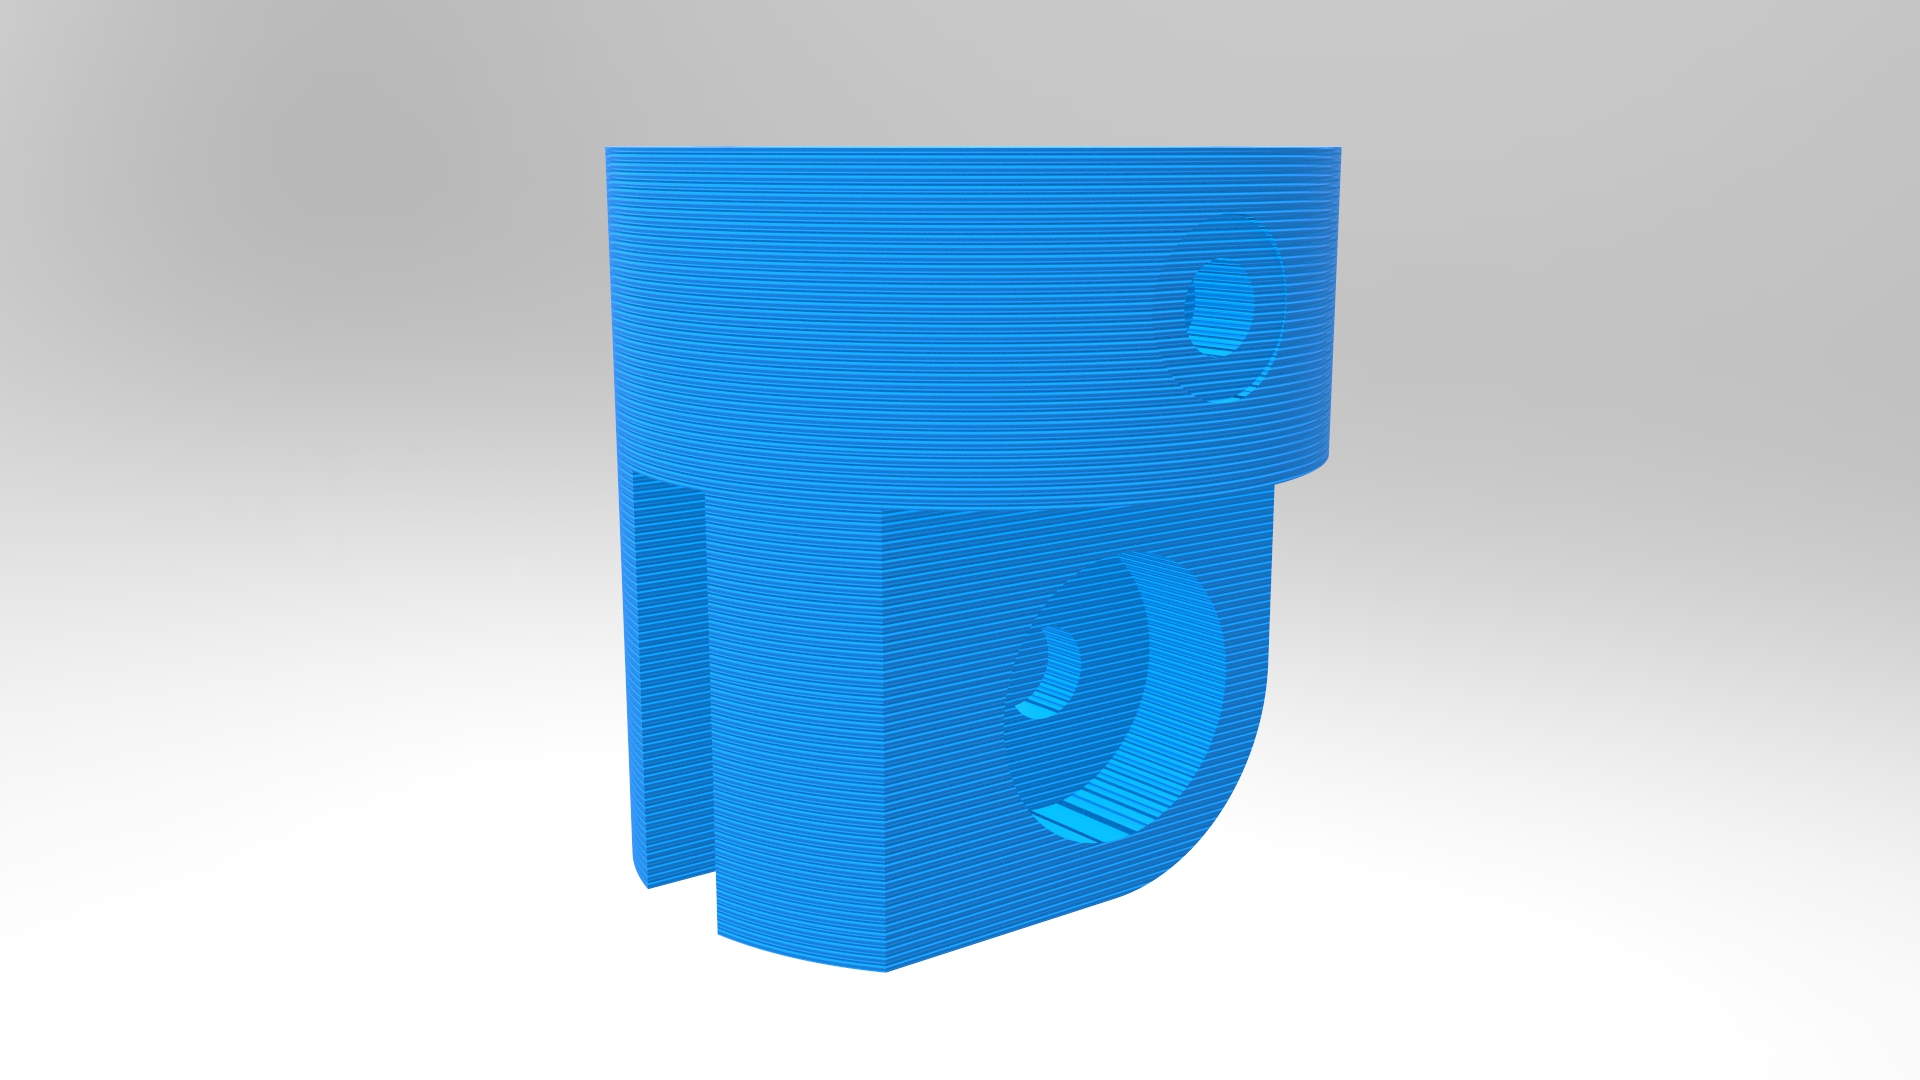
\includegraphics[width=\textwidth]{figures/legs_knee_upper.jpg}
        \caption{Left upper knee}
        \label{fig:knee_upper}
    \end{subfigure}
\end{figure}

% subsection computer_aided_design (end)

% section mechanics (end)
%!TEX root = ../../../report.tex
\section{Software} % (fold)
\label{sec:software}

%!TEX root = ../../../../report.tex

\subsection{Motivation} % (fold)
\label{sub:motivation}
When approaching the task of designing a new robotic platform for the AI department at the Mærsk Mc-Kinney Møller Institute, the current development environment being utilized and its capabilities were studied as a first step.
Nowadays, the simulation and control of the robots at the department is based on the LPZrobots \cite{lpzrobots} and Gorobots \cite{gorobots} packages.
These software tools provide both a simulation engine for robots built on ODE \cite{ode}, OSG \cite{osg} and a framework for an easy implementation of controllers in both simulation and hardware.
However, their specificity compared to other existing instruments collides with some of the core design ideas of the robot framework presented here, which are simplicity of use and generalization.
The above mentioned are the reasons why it was decided to migrate the development environment to ROS Jade \cite{ros} for the bipedal locomotion study framework of RuBy. 

% subsection motivation (end)
%!TEX root = ../../../../report.tex

\subsection{ROS control} % (fold)
\label{sub:ros_control}

% subsection ros_control (end)
%!TEX root = ../../../../report.tex
\subsection{ROS Control-to-Hardware interface} % (fold)
\label{sub:ros_control_hardware_locokit_interface}
The Locokit embedded electronics comes along a standard C library called LocoAPI designed for an easy interaction and use of the capabilities of its hardware, as presented in \cite{locokit}.
This library has been utilized to implement the basic hardware functionalities in Rubi without any modification.
However, it can be easily edited or extended in order to add new ones if needed, which was considered a great advantage during the selection of the hardware platform.

The Locokit can be configured to offer a wireless interface between its main processor and an external computer creating and add-hoc WiFi network in the Gumstix.
Besides, it offers a ready-to-use $C$ application based on the LocoAPI to work as the server side when interfacing the hardware. \ref{} %add actuateMotors.c to code stack?
Its setup and use instructions can be found in the Locokit documentation, supplied with the kit.
This left the client side of the wireless connection as the one that needed to be created.
An existing client application built as an "AbstractController" for the LPZrobots framework was already available. 
However, as explained before, to eliminate any dependency with LPZrobots and in order to use it within ROS Control, it was rewritten as an instantiation of "RobotHW" making use of the LocoKitInterface and ConnectionClass $C++$ classes provided.

\subsubsection{The Locokit HW interface node} % (fold)
\label{ssub:the_locokit_hw_interface}
The resulting ROS node currently implements the functions listed in \ref{list:locoHW_functions}.
They are fully operative and have been tested before assembling the actuators to the joints.

\begin{itemize}
\label{list:locoHW_functions}
	\item Setup of wireless connection: connect to the TCP websocket created in the server side. It requires the IP and port on the server side.
	\item Registration of HW interface handlers for ROS Controller Manager: currently Effort commands and Joint State readings can be transmitted.
	\item Transmission of motor commands to motor boards in HW side: PWM signal values. It requires the physical addresses of all the motor boards connected.
	\item Reception of joint state readings from motor boards: encoder tics for relative position
	\item Real-time handling of information transfer from/to the Controller Manager
\end{itemize}

The node can be extended with new standard/customized HW interface handlers and more functions from the "LocokitInterface" class for future applications.
However, it lacks some capabilities that will be of relevance for an optimal functioning of the Rubi robot and that failed be implemented due to time constraints or lack of resources. 
The main ones are listed in \ref{list:locoHW_functions_left}.

\begin{itemize}
\label{list:locoHW_functions_left}
	\item An initialization of the encoders to a predefined position set as zero in order to compute absolute position values.
	\item A new data flow channel to manage the sensory feedback information from non-built-in sensors, at the ground contact switches.
	\item If necessary, a mapping between the Effort command values received from the controller and the valid PWM signals sent to the motors.  
\end{itemize}
% subsubsection the_locokit_hw_interface (end)

\todo{Add roslaunch explanation in rubi\_bringup package?}

% subsection ros_control_hardware_locokit_interface (end)
%!TEX root = ../../../../report.tex

\subsection{Example controllers} % (fold)
\label{sub:example_controllers}
From the \textit{Controller manager} from ROS Control, different joint controllers can be handled.
In the example controllers the position controller and the effort controllers are used individually for each joint.
This joint controllers offer then a topic (e.g. /rubi/left\_ankle\_position) that the user can use to move the actuators.
This are created from a unique package called \textit{rubi\_joint\_controllers}.
It is worth to say that the position controllers are implemented with a PID and that these values have been adjusted experimentally with the simulations for each joint.

Two type of controllers are given that show a different range of options to use with the robot are presented.
Both are gathered in a sole package called \textit{rubi\_controllers}, which gives a more tidy and resource-shared environment rather than having a package for each controller.
This also makes really easy to deploy a new controller by removing all the creation process of a new package.
In order to start a new piece of code this must be created and then added in the \textit{CMakeLists.txt} from where also some examples are included.

The presented code follows the ROS conventions and the code style is the \textit{Google style} offered by the clang-code-model.
This creates a congruent workspace supervised by a git repository.

\subsubsection{Two neuron controller} % (fold)
\label{ssub:two_neuron_controller}
This first example controller shows how to:
\begin{enumerate}
    \item Use GoRobots.
    \item Make use of dynamic reconfigure.
    \item Adapts its behavior depending on gazebo real time factor.
\end{enumerate}
For the first, an example of how to link C++ code from GoRobots is shown in the \textit{CMakeLists.txt}.
This system is easier and more powerful than the current \textit{Makefiles} currently used in GoRobots.
The Artificial Neuronal Network (ANN) library is used to create a bi-neuronal network that creates the CPG signals of the actuators.
Furthermore, the synaptic weights can be modified by making use of the ROS feature \textit{Dynamic Reconfigurable Parameters}.
These offer an interface in order to change, on the fly, the the values of the created parameters.
In the figure \ref{fig:rqt_interface}, an RQT workspace containing the CPG signals and the dynamic reconfigurable parameters modifiers is depicted.

\begin{figure}[tb]
    \centering
    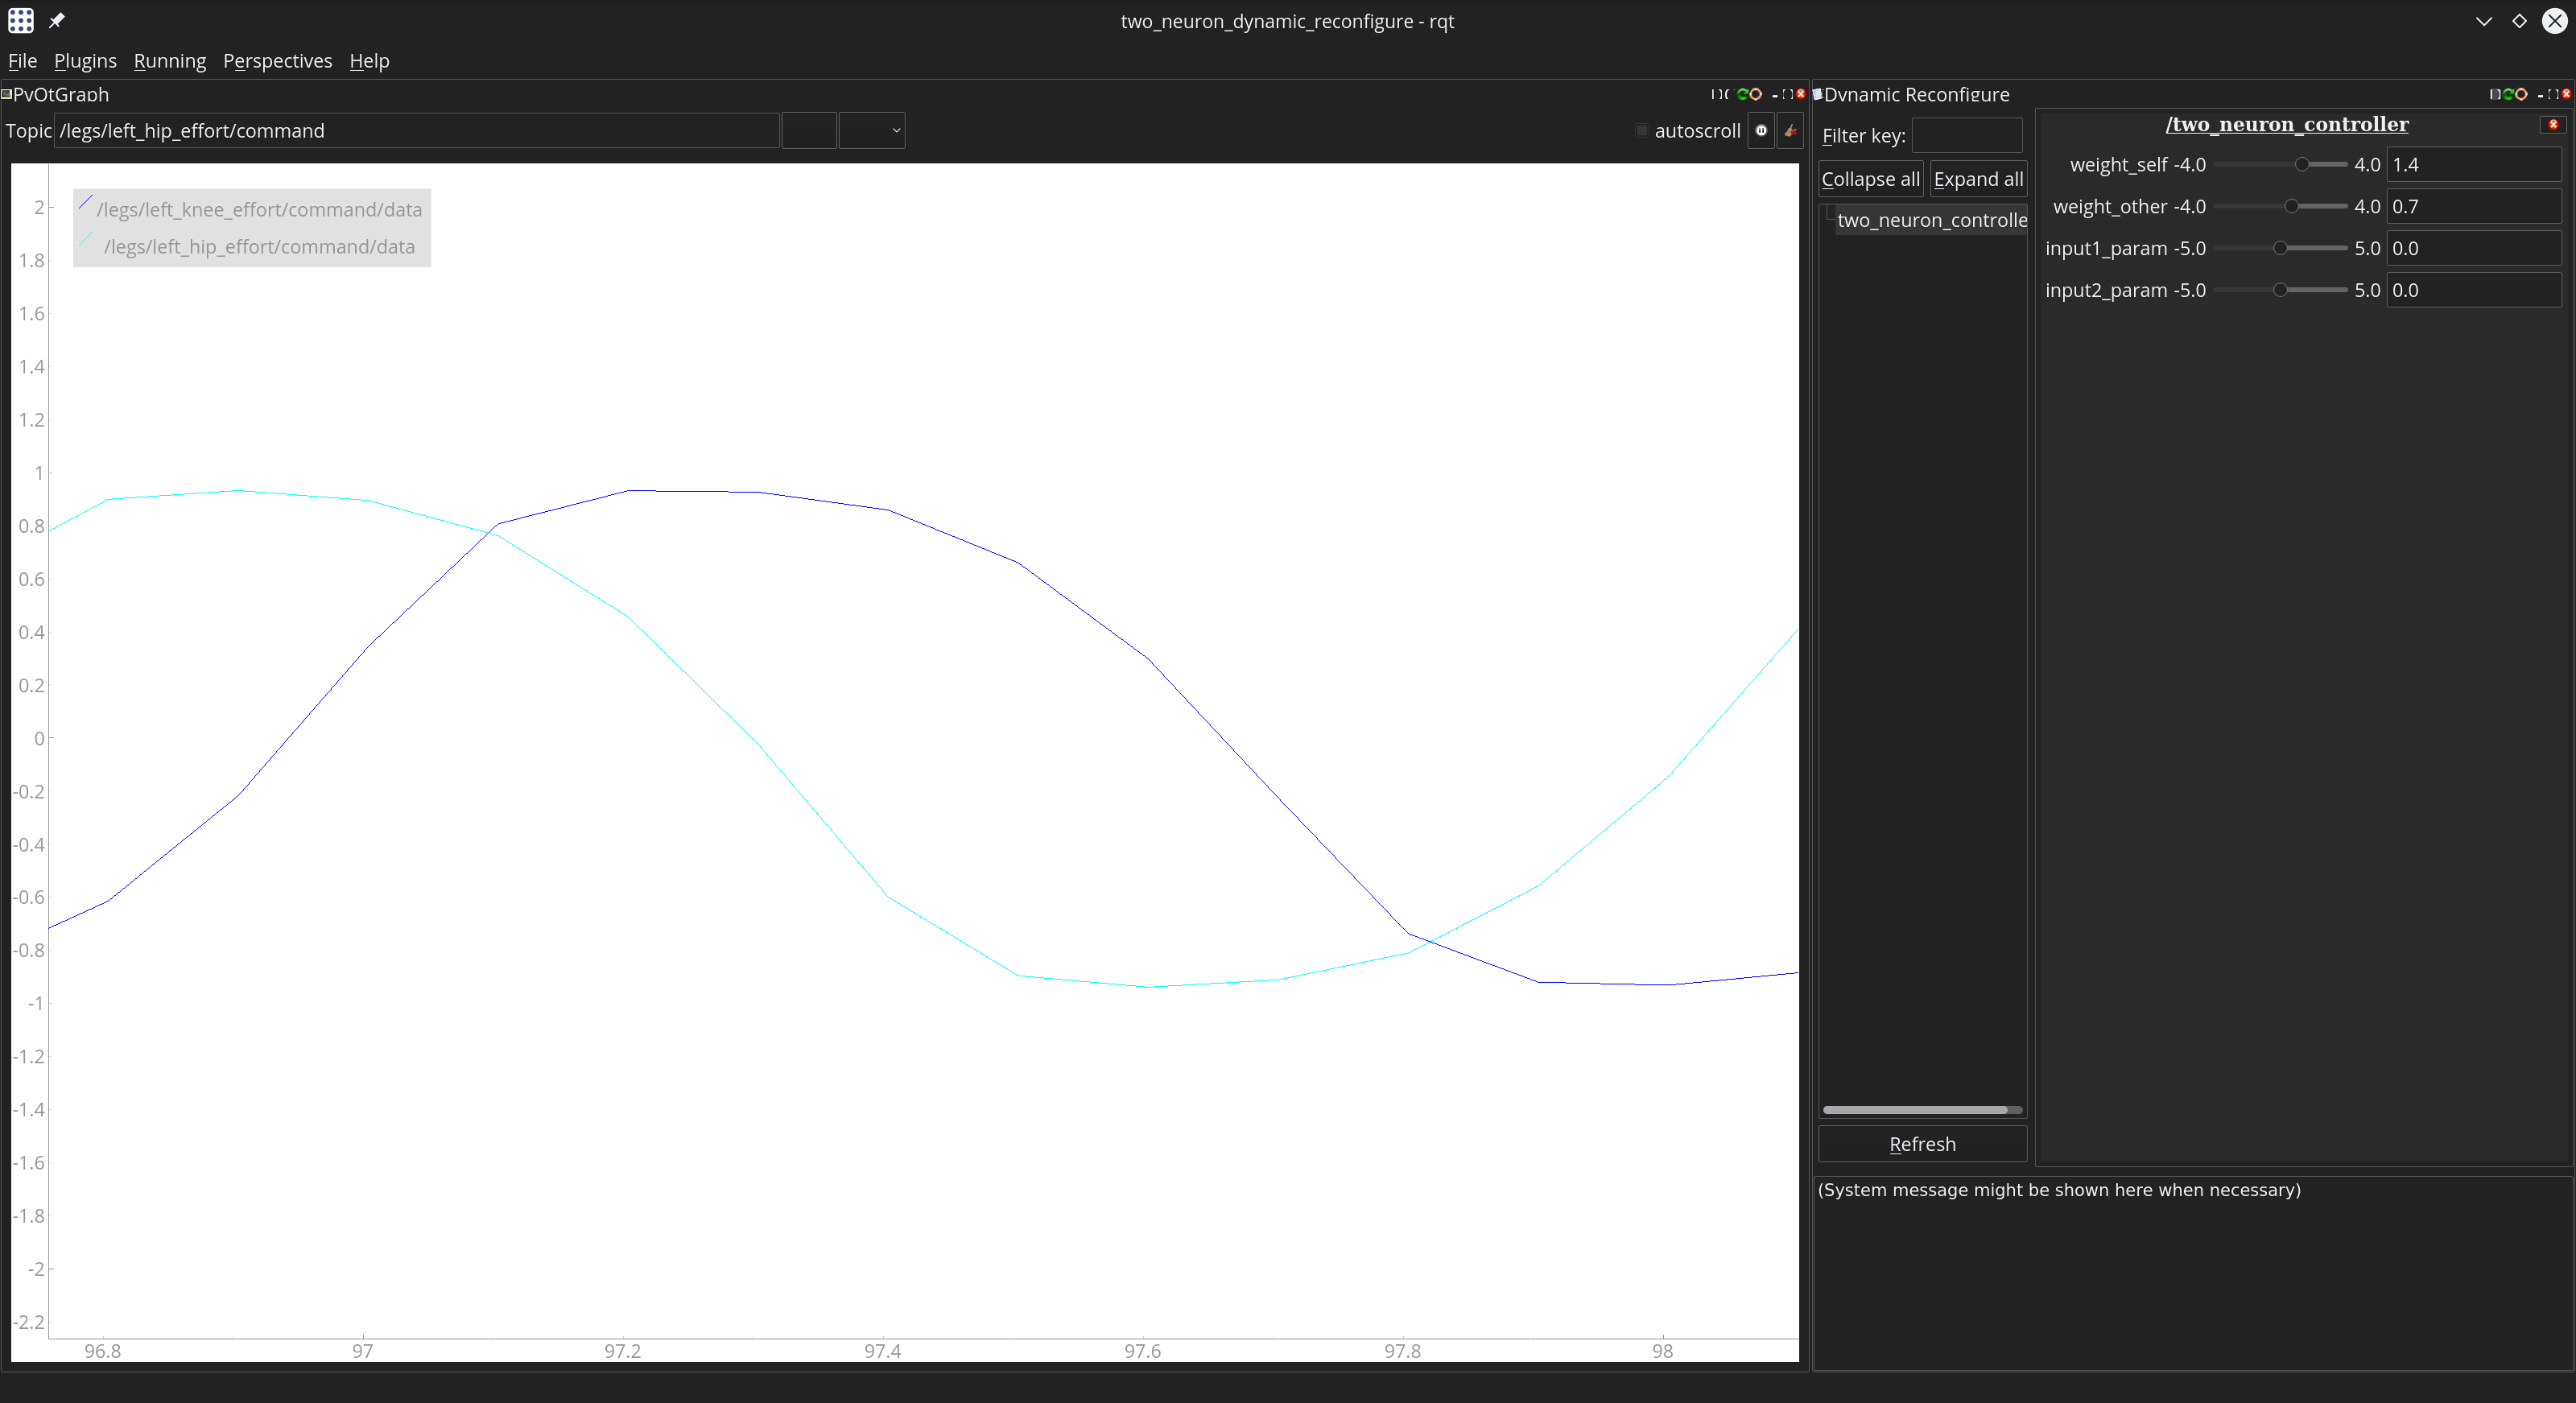
\includegraphics[width=\textwidth]{figures/rqt_interface}
    \caption{RQT workspace containing the CPG signals and the dynamic recofigurable parameters.}
    \label{fig:rqt_interface}
\end{figure}

This are also used to change the behavior of the ANN in order to be adapted to changes in Gazebo.
Gazebo uses can accelerate and decelerate the speed at which the time is passing through.
This is adjusted with a \textit{real time factor} that is read by the node and used to adjust the frequencies of the CPGs.
% subsubsection two_neuron_controller (end)

\subsubsection{Impulse controller} % (fold)
\label{ssub:impulse_controller}
Among other things this node shows how to:
\begin{enumerate}
    \item Load and unload different joint controllers.
    \item Give some wrappings for set of controllers (hoping position).
    \item Offer services for jumping: given a file or given the values and impulse time.
\end{enumerate}
This node implements some methods that enable it to change on-the-fly the controllers of each individual joint.
Furthermore, three combinations of individual joint controllers are given being these: (1) all in position mode, (2) all in effort mode and (3) left leg in position mode and right in effort mode.
The last one is useful when hoping, a moment in which a leg must hold a position and the other keep pushing in order to jump.

Three different services are implemented that impulse the robot in the sake of rise it from the floor.
The first two, are \textit{impulse\_one\_leg} and \textit{impulse\_two\_legs} which given a torque for each joint and an impulse time, it gives the possibility to jump either with one or two legs.
Both services load the necessary joint controllers in order to achieve the desired movements.
The third one offers sort of the same service but the parameters are read from a file instead.
This is handy when combined with the dynamic controller developed in MatLab and explained in the section \ref{sec_dynamic_model}.
% subsubsection impulse_controller (end)

% subsection example_controllers (end)

% section software (end)

% chapter design (end)chapters/cha_design/
    %!TEX root = ../../report.tex

\chapter{Simulation} % (fold)
\label{cha:simulation}
This chapter is meant to answer the questions what, why and how a simulator takes part in the framework.
Starts with a motivation section \ref{sec:sim_motivation} which defines the scope of the simulator
 in the project, followed by a comparison of simulators \ref{sec:sim_comparison_of_simulators} and how to define a robot and its environment in it \ref{sec:robot_definition}; in the next section \ref{sec:robot_creation} is explained how the simulation model of the legs has been created and how to add new features, whilst the creation of the environment is dealt in the section \ref{sec:environment_creation}; finishes with a how-to dedicated section for launching the simulation from scratch in \ref{sec:how_to_simulate}.
%!TEX root = ../../../report.tex
\section{Motivation} % (fold)
\label{sec:sim_motivation}
In the previous chapters the design of a human-proportional biped has been presented. 
The robot has been developed with security systems in both, software and hardware, that prolong the operating life of the robot. 
Nevertheless, every device in real life is prone to suffer damage which translates in to money and time for the user.
By forming part of the toolbox offered in the framework, a comprehensive biped simulation is given so the user can both work with the same algorithms in real and simulated life.

Whilst not being a complete replacement of the real life, it offers a similar experience what allows to do qualitative research.
As an example, neuronal networks or reinforcement learning algorithms, that learn by experience, can be developed faster in the simulator and then transfered to the real robot, reducing the workflow and the need of resources of the user and justifying its use.

A simulator consists basically of two elements: a physical engine and a graphical engine.
Whilst the first one is in charge of calculate all the physical interactions that the agent suffers, the second one offers the visual experience.
A congruent simulator with the presented framework will satisfy two conditions:
\begin{enumerate}
  \item The effort for testing among the simulation and real life must be minimized
  \item The results must be as closer to real life as possible. This includes multiphysics support (mechanical contacts, different aspects of tribology, wind, water...) but within a fair trade-off with computational speed.
\end{enumerate}

% section motivation (end)
%!TEX root = ../../../report.tex
\section{Comparison of simulators} % (fold)
\label{sec:sim_comparison_of_simulators}
When choosing a simulation platform there are several factors to have into account.
Three robotic simulators have been analyzed and compared. 
These are: LPZ Robots \cite{lpzrobots} (Figure \ref{fig:lpzrobots_example}), V-Rep \cite{vrep} (Figure \ref{fig:vrep_example}) and Gazebo \cite{gazebo} (Figure \ref{fig:gazebo_example}).
Some comparisons can be found in the literature as \cite{nogueiracomparative} or \cite{staranowicz2011survey} however the predominant criteria has been their integration with ROS.

\begin{figure}[hb!]
  \begin{subfigure}{.33\textwidth}
    \centering
    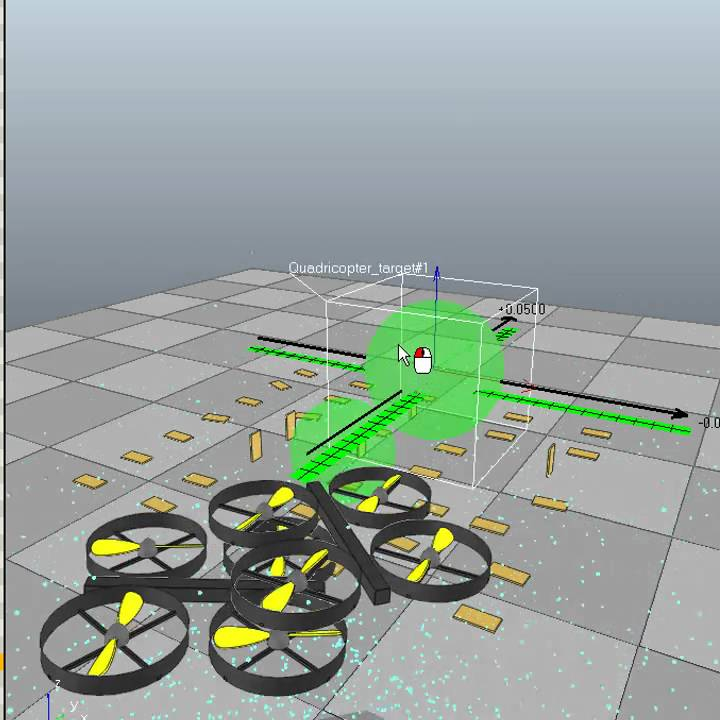
\includegraphics[width=.95\linewidth]{figures/vrep_example}
    \caption{V-Rep}
    \label{fig:vrep_example}
  \end{subfigure}%
  \begin{subfigure}{.33\textwidth}
    \centering
    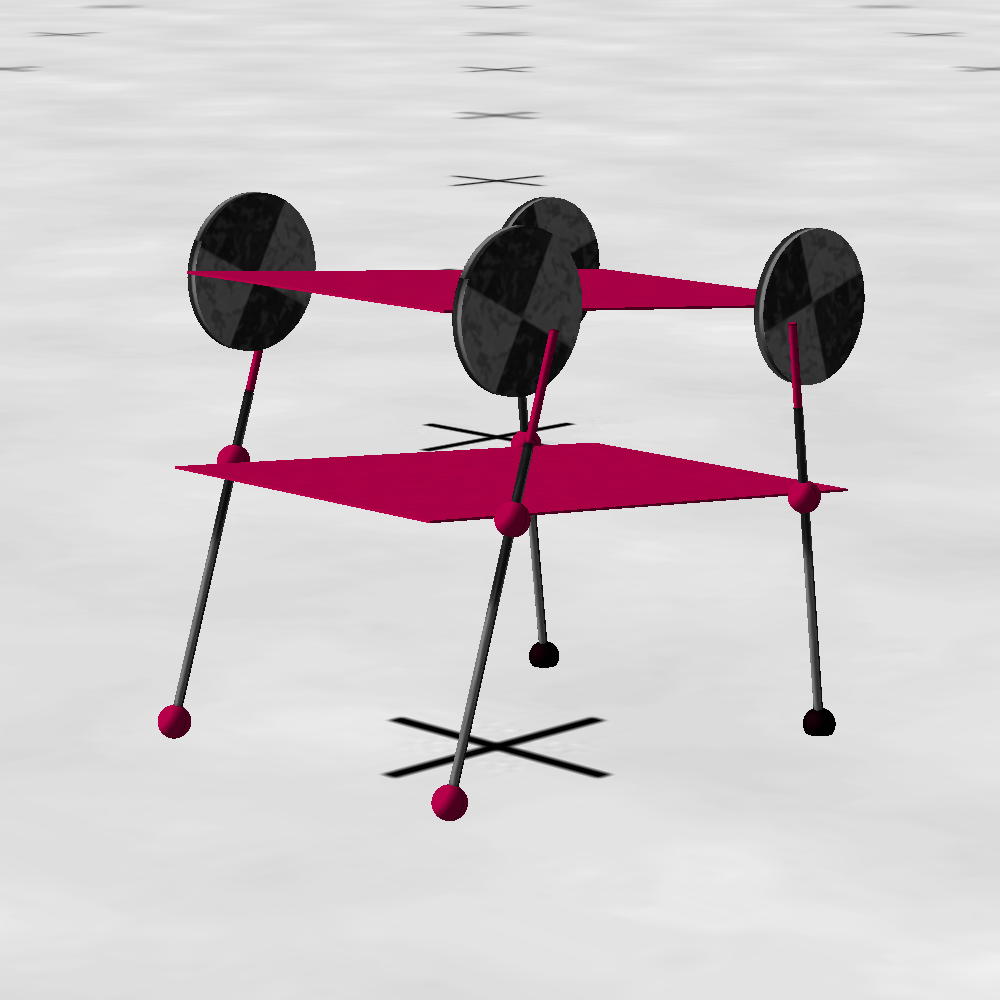
\includegraphics[width=.95\linewidth]{figures/lpzrobots_example}
    \caption{LPZ Robots}
    \label{fig:lpzrobots_example}
  \end{subfigure}
  \begin{subfigure}{.33\textwidth}
    \centering
    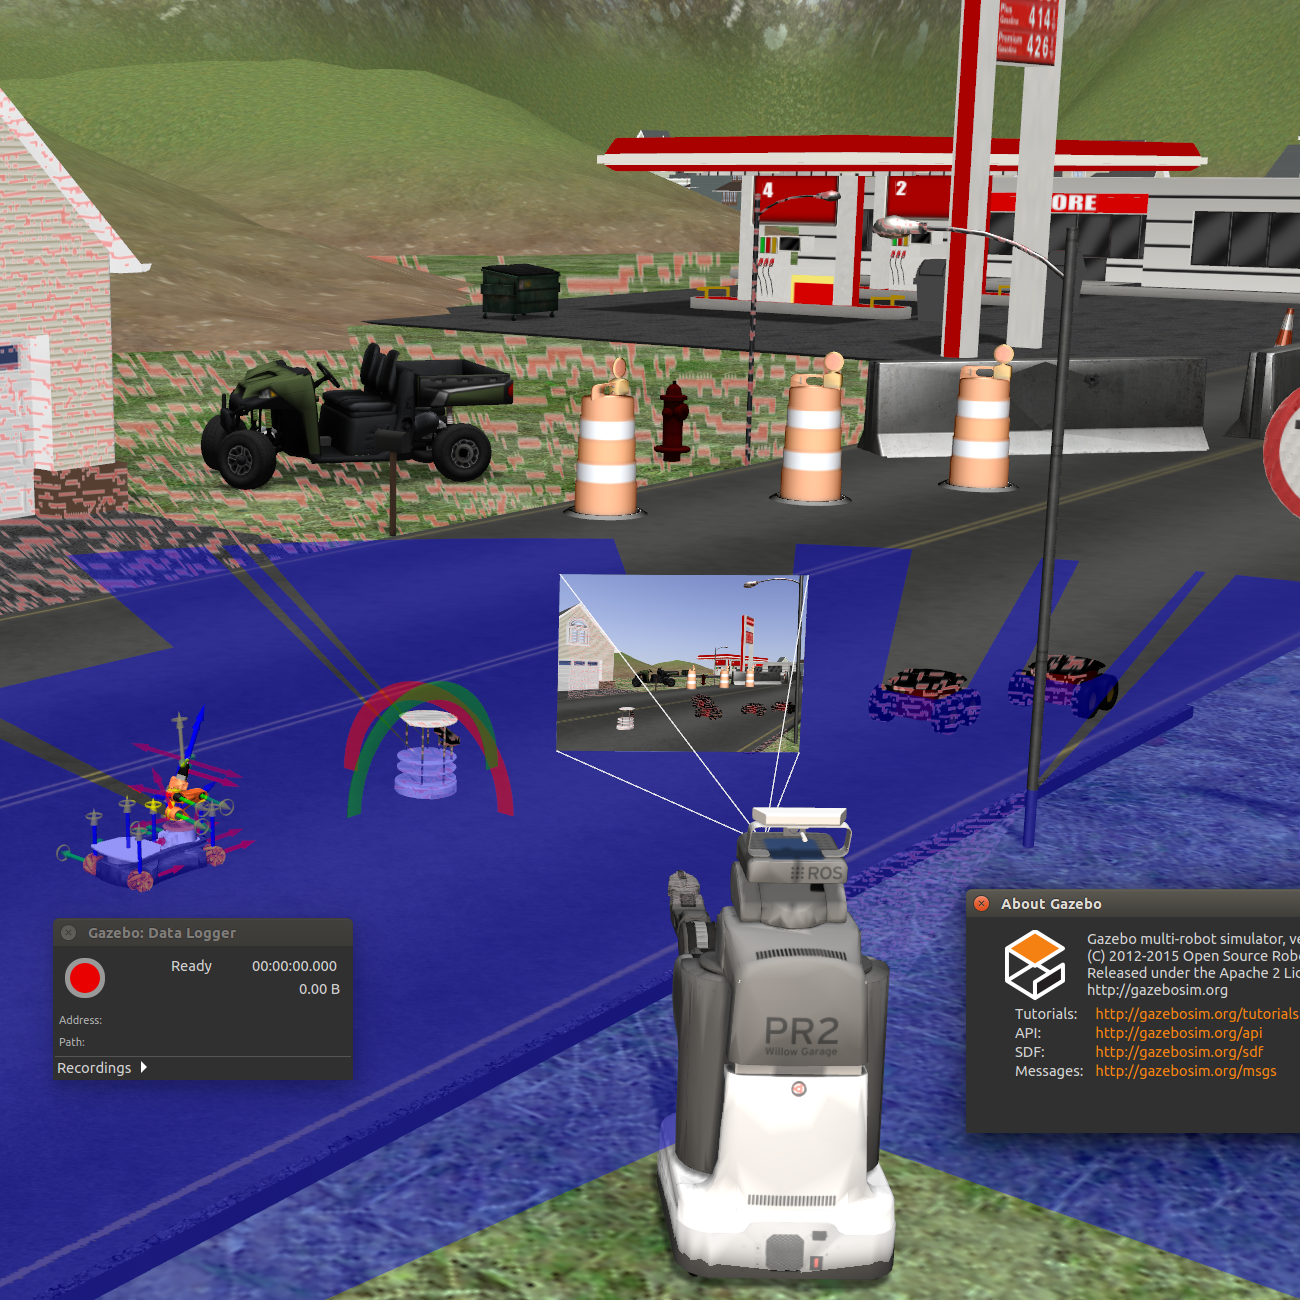
\includegraphics[width=.95\linewidth]{figures/gazebo_example}
    \caption{Gazebo}
    \label{fig:gazebo_example}
  \end{subfigure}
  \caption{Simulation examples of the software analyzed.}
  \label{fig:simulation_comparison}
\end{figure}

The RuBi robot is mainly targeted to be used in the AI department at the Maersk Mc-Kinney Møller Institute, where the toolbox GoRobots is being developed.
This is a set of tools, from a neuronal networks API to a genetic algorithm engine, written in C++ than is meant to be simulator-independent.
However, in order to provide a more general and supported simulation and development environment for the user, ROS Jade \cite{ros} has been selected as the tool to use.
The whole set of instruments provided in ROS along with its easy extendability give the opportunity to use the controllers and tools already developed in GoRobots.
Despite the fact that the three simulators compared have a C++ interface that would allow to interface them with ROS, Gazebo is already fully supported and integrated in ROS, making it the logic choice.
This reduces the learning curve of a new user and the installation process is easier due to it is included in the Open Source Robotics Foundation (OSRF) repositories.

Regarding the second condition, Gazebo has the feature of changing the physics engine in the beginning of the simulation, it has multiphysics support (fluids, electromagnetism...), it allows to load external geometries from STL or Collada and, the most important, has an active community behind it providing support and documentation. These are the reasons for selecting Gazebo as the simulator for the RuBi platform.
In \cite{physics_engine_gazebo_comparison}, a comparison with the different physical engines is carried out.
For the sake of simplicity the default one, Open Dynamics Engine (ODE), has been used, although the others have been tested.

% section comparison_of_simulators (end)\[
%!TEX root = ../../../report.tex
\section{Robot definition} % (fold)
\label{sec:robot_definition}
As in May of 2016, ROS Jade ecosystem has different formats to describe a robot.
These are SDF, URDF and Xacro.
At some point they are all transformed to a unique sort of format but the decision of how to express the robot for the simulation is needed from the beginning.


\begin{enumerate}
  \item \textbf{URDF \footnote{http://wiki.ros.org/urdf}}: is an open standard used in all the simulators mentioned or others like RobWork \cite{robwork}. 
  It allows to define all the properties of a single robot but lacks other which are important when simulating. 
  It is mainly used for visual representations or schematic robot definitions.
  \item \textbf{Xacro \footnote{http://wiki.ros.org/xacro}}: is a parametric format that easy the writing of the URDF.
  It allows logic conditions like \textit{if, for} and from ROS Jade any virtual python condition.
  This code is then compiled into a URDF automatically which give Xacro complete interoperability with URDF readers.
  \item \textbf{SDF \footnote{http://sdformat.org}}: adapted to the current requirements of the simulation environments.
  With it can be defined from \textit{worlds} to air properties in the case or UAV simulations.
\end{enumerate}

Despite SDF contains more information, there are several tools in ROS Jade that make use of URDF.
Two of them are RViz and ROS Control, explained in the section \ref{sub:ros_control}.
As this last one is a pillar of the framework itself, the decision of making use of URDF as format for describing the robot was taken.
However, the robots developed have been written in Xacro due to the tools that easy the coding of the robot.
% section robot_definition (end)
%!TEX root = ../../../report.tex
\section{Robot creation} % (fold)
\label{sec:robot_creation}
One of the goals of the framework is to easy its continuity, thus this section is dedicated to explain how the robot was created.

A robot is defined as a set of links jointed.
A link contains at least three blocks of information:
\begin{enumerate}
   \item The collision model: used to calculate the collisions with other agents in the simulation.
   \item The visual model: uniquely used for visual purposes.
   \item The inertial information: defines physical properties like the mass and the moments of inertia of the link.
\end{enumerate} 

A trade-off must be found for the precision of the collision model between accuracy and speed.
The more detailed is the model, the higher will be computation time which translates into more accuracy and more computation time.
The general advice is to have two simulation models: one for visual purposes and the other one for collisions.

In the case of the links of presented robot, the visual models are obtained directly by exporting the parts from SolidWorks whilst the collision models are made of primitive gazebo shapes (cubes, cylinders, spheres...) for the whole body but the feet.
Due to the robot is not meant to hit anything, the possible collisions in the body are not a priority, then each link is represented as a cylinder of the same length of the CAD model and of a radius enough to cover the whole part.
An example can be seen in the figure \ref{fig:collision_model}.

The moments of inertia of each individual link are obtained directly from SolidWorks.
The CAD model includes the materials and thus the masses.
From these, the program is able to calculate the moments of inertia.
The figure \ref{fig:moments_of_inertia} shows the representation of these in the simulation.


\begin{figure}[hb!]
  \centering
  \begin{subfigure}{.45\textwidth}
    \centering
    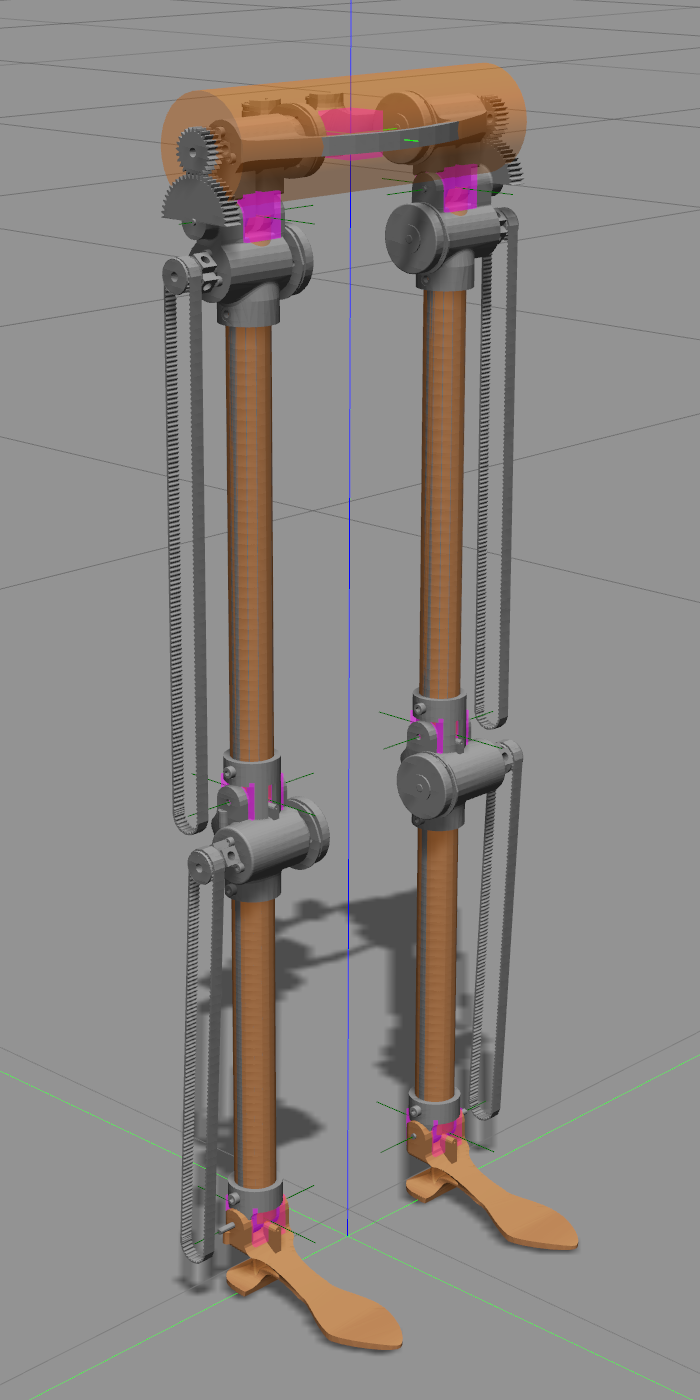
\includegraphics[width=.5\linewidth]{figures/gazebo_collision_model.png}
    \caption{Gazebo showing the visual model, the moments of inertia and the collision model}
    \label{fig:collision_model}
  \end{subfigure}
  \begin{subfigure}{.45\textwidth}
    \centering
    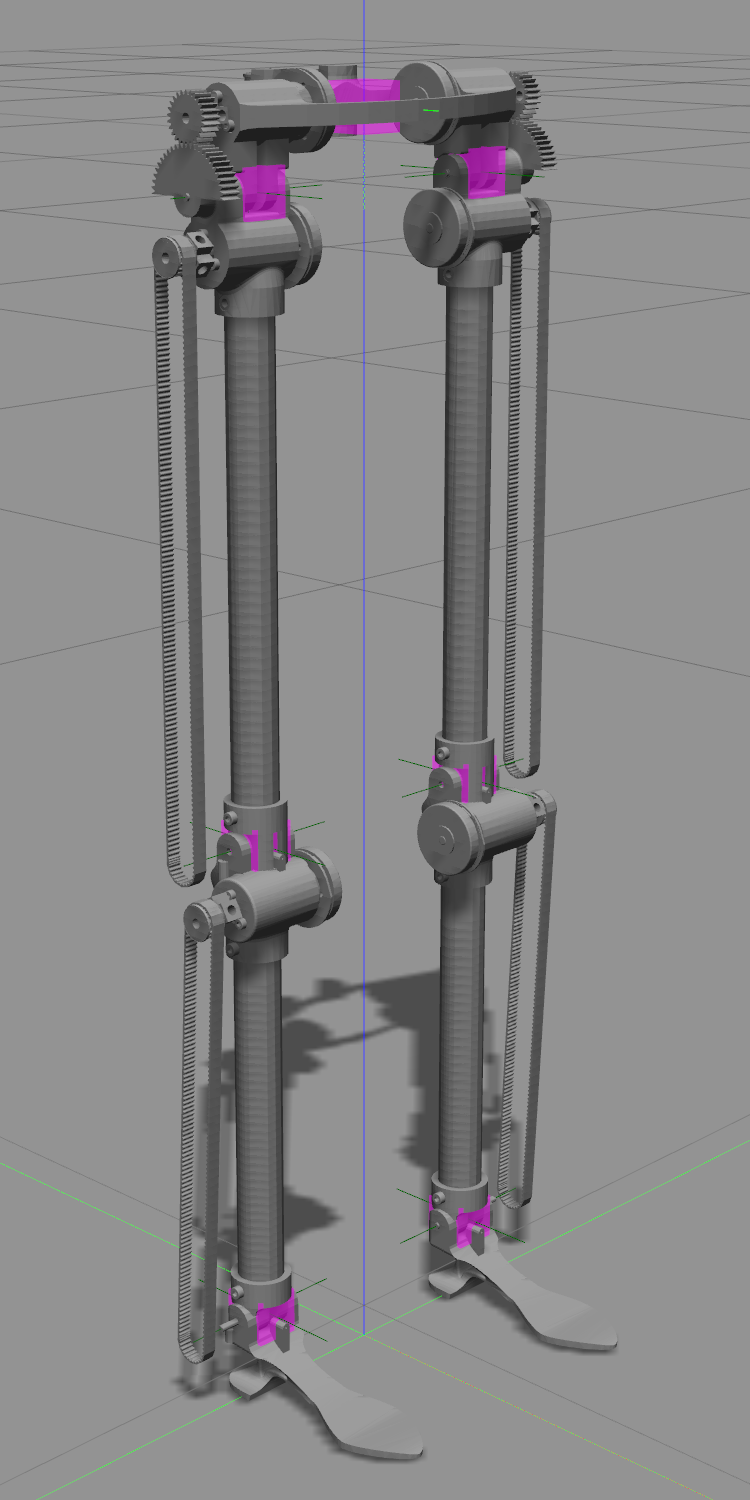
\includegraphics[width=.5\linewidth]{figures/gazebo_intertia_moments.png}
    \caption{Gazebo showing the visual model and the moments of inertia}
    \label{fig:moments_of_inertia}
  \end{subfigure}
\end{figure}

It is important to notice that the visual models and moments of inertia have been exported from the correct coordinate system.
In the case of the ankle, for example, the STL file and the moments of inertia are calculated from the coordinate system positioned in the middle of the rotational axis of the ankle, pointing the Z axis to the rotational axis and Y to the biggest extension of the part.
This can be seen in the figure \ref{fig:solidworks_ankle_coodinate_system}.

\begin{figure}[ht!]
  \centering
  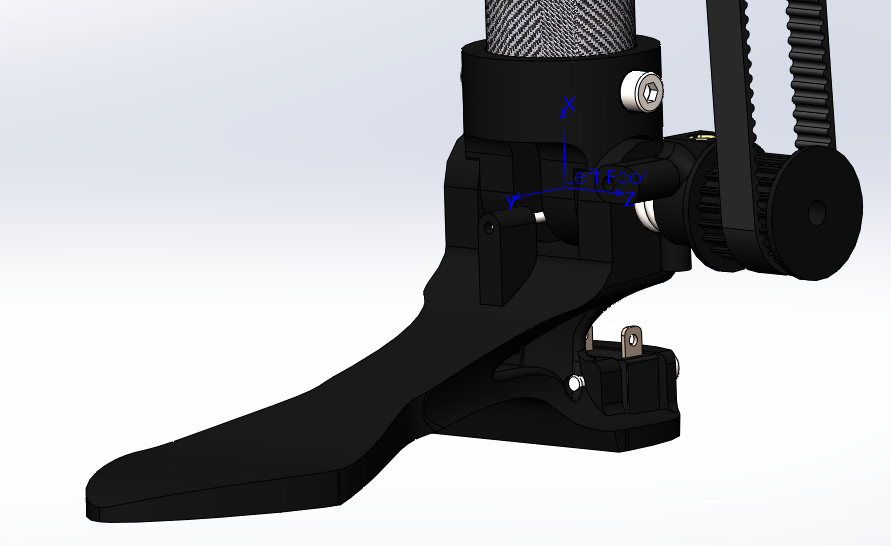
\includegraphics[width=0.75\linewidth]{figures/solidworks_ankle_coordinate_system}
  \caption{Coordinate system of the left ankle in SolidWorks}
  \label{fig:solidworks_ankle_coodinate_system}
\end{figure}

Finally, in the Xacro file the information that lacks the URDF must be added in order to simulate with Gazebo.
Eventually, to the RuBi description is added:
\begin{enumerate}
  \item \textbf{Plug-in for ROS Control}: Offers an interface for using ROS Control inside Gazebo.
  \item \textbf{Contact sensors}: Simulates contact sensors as in the feet of the real robot.
  \item \textbf{Defines friction of the components}: as the friction between the feet and the floor.
\end{enumerate}

% section robot_creation (end)
%!TEX root = ../../../report.tex
\section{Dimensional analysis} % (fold)
\label{sec:dimensional_analysis}
A problem came up when creating the robot. 
Some of the inertia moments obtained from SolidWorks, were in the order of magnitude of $10^{-8}$.
Such small number is not handled by the physics engine correctly causing the robot model to be unstable under normal conditions.

Three approaches were taken:
\begin{enumerate}
  \item \textbf{Change the physics engine}: As commented in the simulation comparison \ref{fig:simulation_comparison}, Gazebo supports multiple physics engines. Dart \cite{dart}, Simbody \cite{simbody}, Bullet \cite{bullet} and ODE \cite{ode}, where tested giving the same unstable behavior. 
  Thus, this method was discarded.
  \item \textbf{Fake the moments of inertia}: This would be to make 0 the really small moments of inertia and only leave the ones over a threshold.
  As the simulation is a qualitative analysis and no quantitative, an exact match of the moments of inertia is not needed. 
  \item \textbf{Dimensional analysis}: Based on \cite{dimensional_analysis}, the size of the robot can be increased in a proportion that make the figures big enough to be handled.
\end{enumerate}

Dimensional analysis can be applied to correlate the physical properties of the original robot with its scaled replica.
This is, if the original robot with mass $m$, volume $V$ and moment of inertia about an axis $I$, given a scale factor $s$, calculate the scaled replica $m'$, $V'$, $I'$ depending exclusively on $s$.

In the equation \ref{eq:general_inertia}, the generalized expression of the moment of inertia about an axis is shown.
\begin{equation}
\label{eq:general_inertia}
  I = \iiint_V \rho(u,v,w) |r^{2}| \,dx\,dy\,dz
\end{equation}

If the equation \ref{eq:general_inertia} is taken as the moment of inertia from the first link, the scaled one would be the shown in the equation \ref{eq:general_inertia_2}:
\begin{equation}
\label{eq:general_inertia_2}
  I' = \iiint_{V'} \rho(u,v,w)' |r^{'2}| \,dx'\,dy'\,dz'
\end{equation}

Supposing a scale factor of $s$ and as stated in the equations from \ref{eq:dx} to \ref{eq:dz}:

\begin{multicols}{3}
  \begin{equation}
  \label{eq:dx}
    \,dx=s \,dx'
  \end{equation}\break
  \begin{equation}
  \label{eq:dy}
    \,dy=s \,dy'
  \end{equation}\break
  \begin{equation}
  \label{eq:dz}
    \,dz=s \,dz'
  \end{equation}\break
\end{multicols}

Then can be deduced that $r$ increases proportionally with $s$ as shown in the Figure \ref{fig:dimensional_analysis} and presented in the equation \ref{eq:dr}:
\begin{equation}
  \label{eq:dr}
  \,r=s \,r'
\end{equation}

\begin{figure}[ht!]
  \centering
  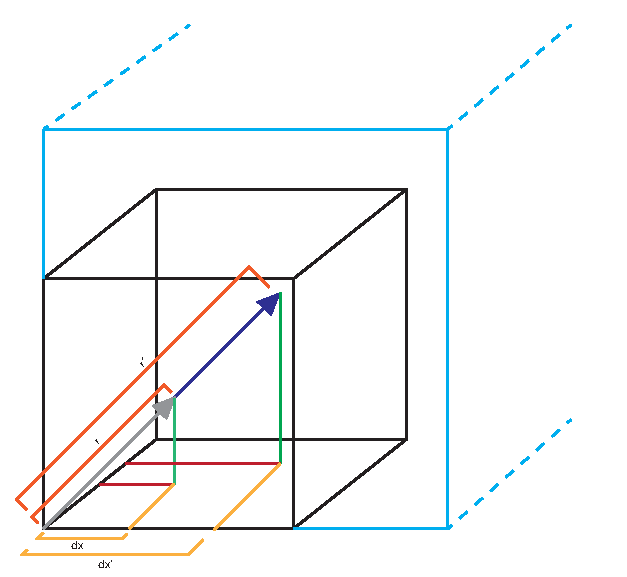
\includegraphics[width=0.5\linewidth]{figures/dimensional_analysis.pdf}
  \caption{Representation of a minimal volumentric cube.}
  \label{fig:dimensional_analysis}
\end{figure}

Assuming a constant density across all the scaled bodies, and particularizing for the moment of inertia of the center of gravity the moment of inertia is given then by \ref{eq:general_inertia_3}:
\begin{equation}
  \label{eq:general_inertia_3}
  I'_{CG} = \iiint_{V'} \rho(u,v,w)' |r^{'2}| \,dx'\,dy'\,dz' = s^{3} r_{CG}^{'2} m
\end{equation}

A correlation can be obtained for the inertia then as shown in \ref{eq:inertia_scale}:

\begin{equation}
\label{eq:inertia_scale}
  I' = \frac{s^{3} r_{CG}^{'2} m}{r_{CG}^{2} m} I = s^{5} I
\end{equation}

And lately the mass can be correlated as in \ref{eq:mass_scale}:
\begin{equation}
\label{eq:mass_scale}
  m' = V' \frac{m}{V} = s^{3}m
\end{equation}

As explained in the \ref{sec:robot_definition}, by using the Xacro format, mathematical expressions can be used.
The definition of the robot includes a set of variables in which is included $scale$ that is used to calculate $mass\_scaled$ and $inertia\_scaled$ that will modify the values of all the links to make a coherence scalable robot definition.

% section dimensional_analysis (end)
%!TEX root = ../../../report.tex
\section{Environment creation} % (fold)
\label{sec:environment_creation}
Besides the robot, other elements can be added to the simulated world.
From the Gazebo database, other robot models or parts (as a beer or a brick) can be inserted and used for any kind of experiments.

\begin{figure}[hb!]
  \centering
  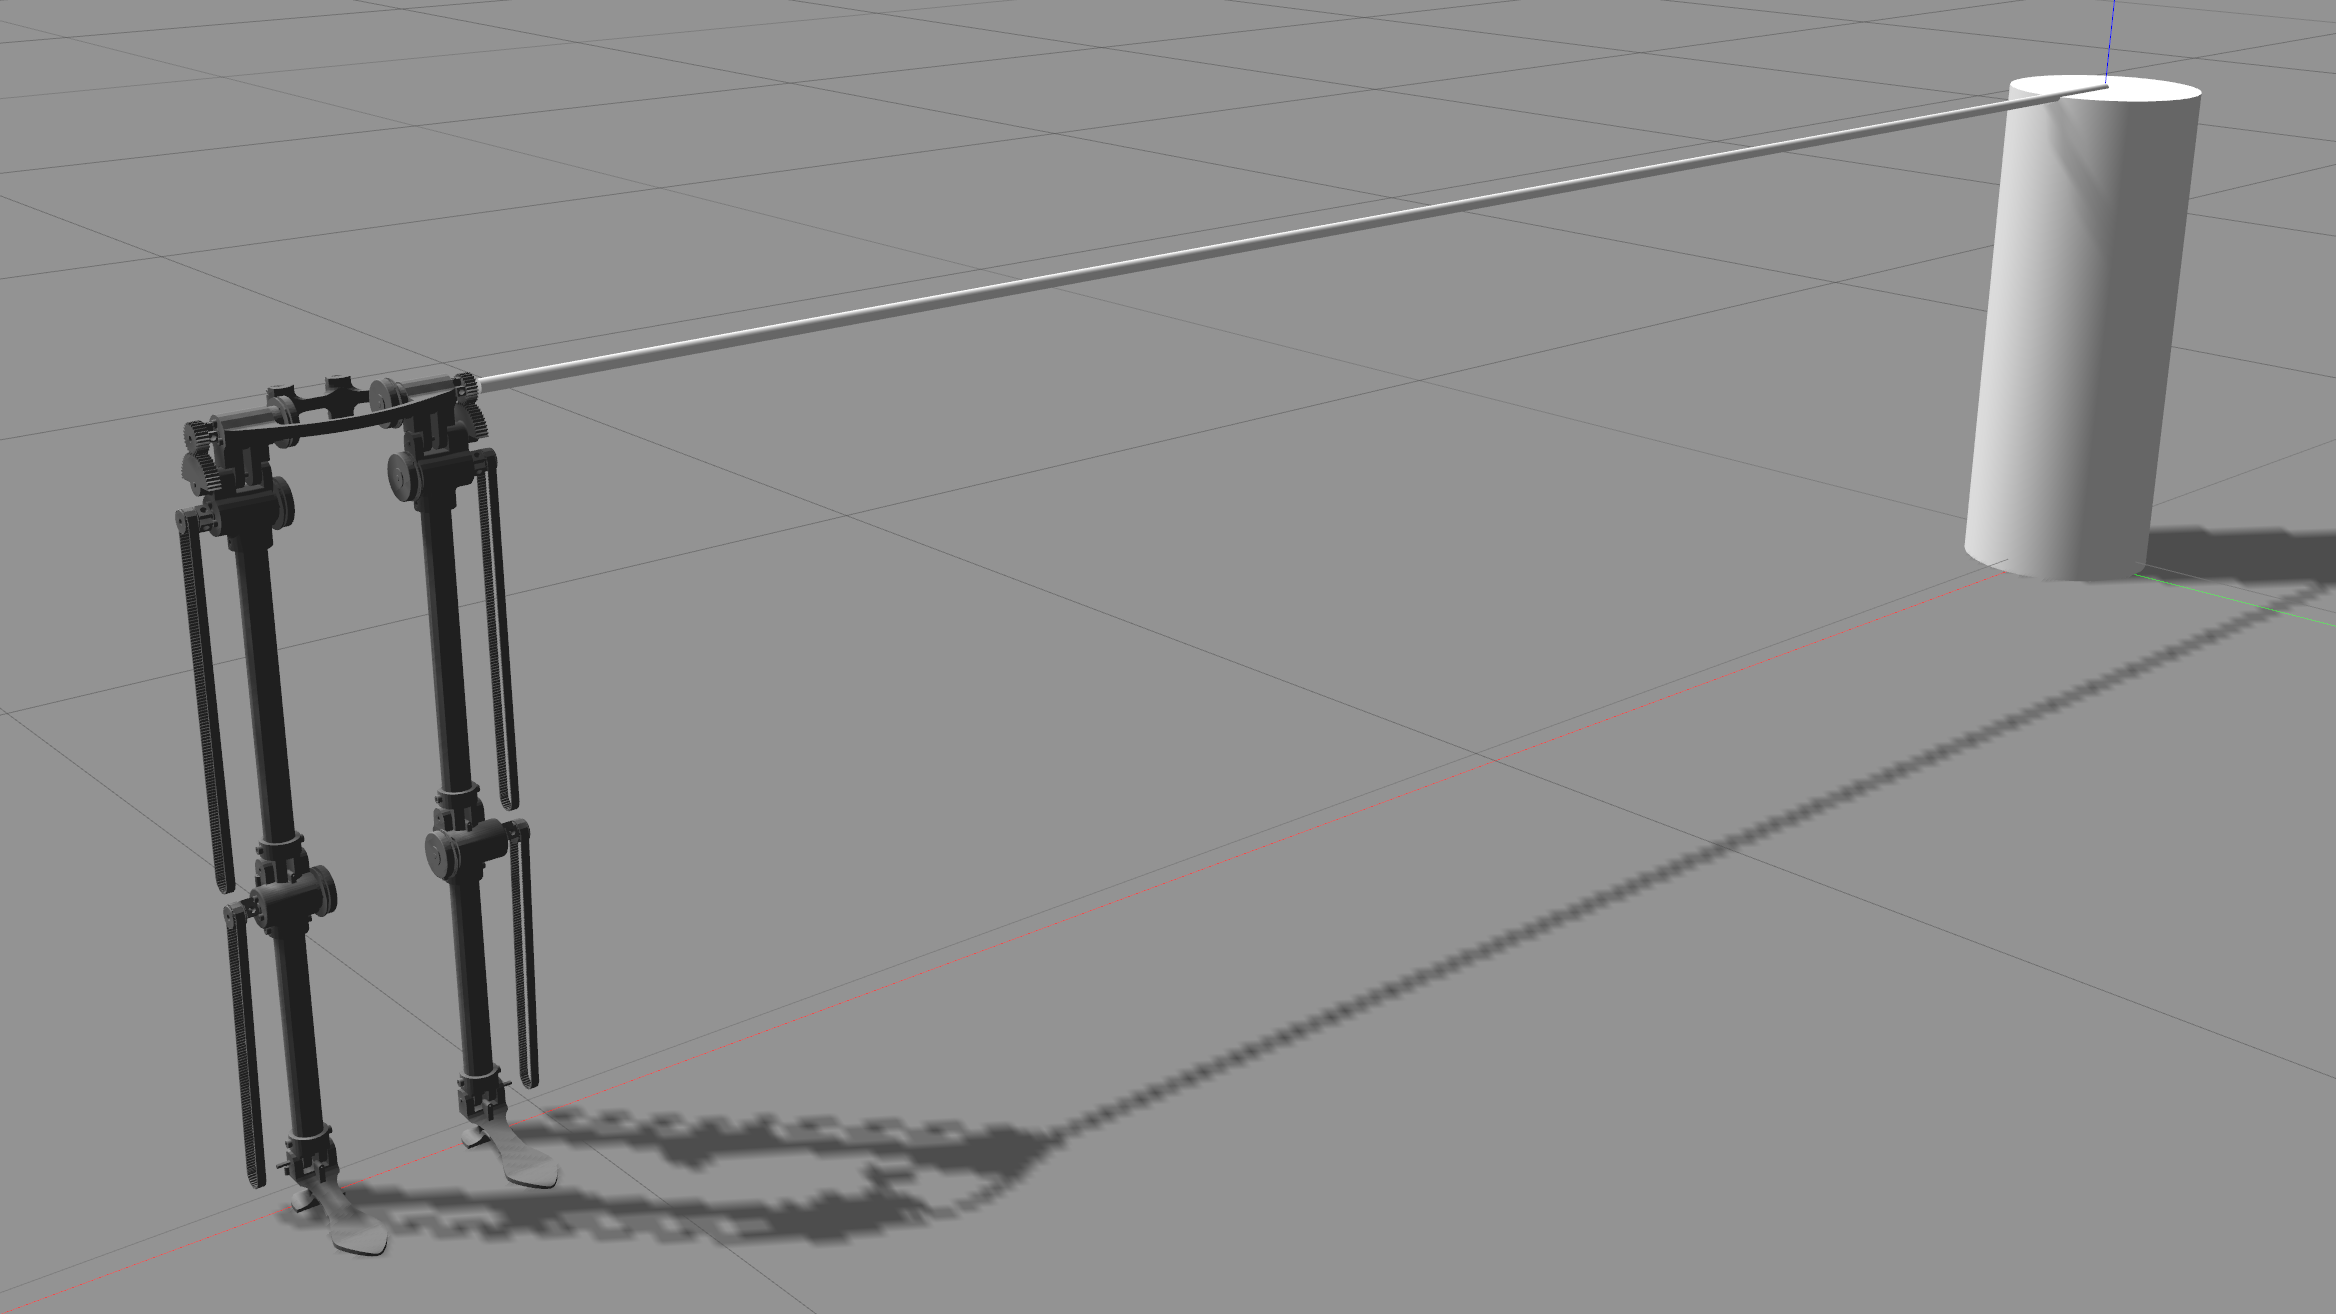
\includegraphics[width=0.75\linewidth]{figures/gazebo_rotational_holder}
  \caption{Rotational robot holder and robot}
  \label{fig:rotational_robot_holder}
\end{figure}

\hfill

In the final framework an extra tool is provided: a rotational robot holder.
It is inspired in the DACbot simulation environment in LPZ Robots, being fully parametric and reducing the degrees of freedom of the robot to constraint its motion to the scenario under study.
It can be seen in Figure \ref{fig:rotational_robot_holder}.

% section environment_creation (end)
%!TEX root = ../../../report.tex
\section{How to simulate} % (fold)
\label{sec:how_to_simulate}
The actions for starting the simulation are minimal and, with everything installed, just a terminal shall be opened and the user have to insert:

\begin{lstlisting}
roslaunch legs_gazebo legs_world.launch
\end{lstlisting}

The launch file will load ROS Control along with the simulation.
From that moment the user can run the controllers and the legs will move equally than in the real robot.
% section how_to_simulate (end)

% chapter simulation (end)

    %!TEX root = ../../report.tex
\chapter{Construction process} % (fold)
\label{cha:implementation}
This chapter is dedicated to explain the process of manufacturing and assembling the introduced designs.
From the important role of emerging low-cost technologies like FFF 3D printing up to the creation of custom PCBs for reducing the weight of the robot, the following sections are meant to explain the process of acquisition and construction of all the components of RuBi presented in previous chapters.
The implementation of the final prototype has always been led by criteria of security, constrained budget and feasibility for maintenance and futures improvements.

%!TEX root = ../../../report.tex
\section{3D printing} % (fold)
\label{sec:3d_printing}
The parts modeled for the project and shown in the section \ref{sub:computer_aided_design}, have been printed using Fused Filament Fabrication (FFF).
The 3D printer used is a M Prime One \footnote{https://github.com/M-Prime/M_Prime_One} with a 0.4 mm noozle.
All the parts have been printed at 0.2 mm layer height.

The use of this technology is justify by the fact that makes the iterative process between design and manufacturing both fast and cheap.
All the parts have been individually adjusted until the clearances have been as expected.
Furthermore, this enable the user not only to replicate the parts with out any considered extra cost, but allows the robot to be easily replicated in other places.

When manufacturing, some of the parts have needed material support.
The figure \ref{fig:photo_material_support} depicts two feet, one with material support and the other with it removed.
In the figure \ref{fig:photo_3d_printed} a detail of actual parts 3D printed and assembled in the robot are shown.

\begin{figure}[ht]
    \centering
    \begin{subfigure}[b]{0.49\textwidth}
        \includegraphics[width=\textwidth]{figures/photo_material_support.jpg}
        \caption{Feet with and without material support}
        \label{fig:photo_material_support}
    \end{subfigure}
    \begin{subfigure}[b]{0.49\textwidth}
        \includegraphics[width=\textwidth]{figures/photo_3d_printed.jpg}
        \caption{Detail of 3D printed parts assembled}
        \label{fig:photo_3d_printed}
    \end{subfigure}
\end{figure}

  \subsection{Arc compensation} % (fold)
  \label{sub:arc_compensation}
  For the CAD models of the 3D printed parts, the clearances of the internal holes have been adjusted following \cite{arc_compensation}.
  The undersizing of internal holes is a common problem in this sort of technology due to the lack of information of the common-used exporting format: the STL.
  This only contains the 3D model expressed as a set of external triangles, which difficult the correction of malformations inherent to the technology.

  In the case of the Fused Filament Fabrication (FFF), the material is extruded equally in both sides of the arc, as shown in \ref{fig:arc_compensation}. 
  However, in the side of the smaller curve, less material is needed.
  This correction can be calculated with:
  $$ r=\frac{t+\sqrt{t^2+4R^2}}{2}$$
  being:
  \begin{enumerate}
    \item t: noozle diameter
    \item R: desired internal hole radius
    \item r: corrected radius
  \end{enumerate}
  As an example, Klee suggests an internal hole of 4.4 mm in the case of the selected nuts \cite{klee}. Thus, the diameter in the CAD model has been adjusted for this data and a noozle of 0.4 mm. The result is then:
  $$ d=2r=\frac{t+\sqrt{t^2+4R^2}}{2}=0.4+\sqrt{0.4^2+4*2.2^2}=4.81$$

  \begin{figure}[tb]
    \centering
    \includegraphics[width=0.5\textwidth]{figures/Arc-compensation}
    \caption{Technical representation of the generated arc when using FFF technology}
    \label{fig:arc_compensation}
  \end{figure}
  % subsection arc_compensation (end)

% section 3d_printing (end)
%!TEX root = ../../../report.tex
\section{Machining} % (fold)
\label{sec:machining}
Along with 3D printing, other parts have needed to be machined.
As an example, the rods came in bars of one meter that have been cut and filed according the design.
Other example are the carbon fiber tubes.
These have been designed to carry the wiring inside them.
Thus some holes have been performed in the bottom and top part of the tube in order to insert them.
The drawings for such parts are included as appendices in \ref{app:mechanical_drawings}.
% section machining (end)
%!TEX root = ../../../report.tex
\section{PCBs and wiring} % (fold)
\label{sec:pcbs_and_wiring}

% section pcbs_and_wiring (end)
%!TEX root = ../../../report.tex
\section{Providers} % (fold)
\label{sec:providers}
In addition to the 3D printed and machined parts, other items have been bought from several providers.
The providers have been selected based on previous shoppings made by the Mærsk Mc-Kinney Møller Institute.
All the needed items that could have followed an standard have been chosen. 
As an example, the robot only needs three types of screws (only M3 metric) and one kind of bearing.
The components are easily found and are not rare items or exotic materials that increase the price of the robot.
A list with all the components bought and its providers is attached as an appendix in \ref{app:order_list}.

As explained in the management of the project \ref{sec:project_management}, all the parts that are bought, included the springs, are ordered in the end of April. 
This was decided due to the delivery of the parts is a process that can take up to three weeks.
Despite all the parts where got within the first week, the springs have not been received, what has impeded the complete assembling of the robot.
However their fastening is easily made by following the assembly manuals provided and other experiments in which the springs are not needed will be carried out.

% section providers (end)
%!TEX root = ../../../report.tex
\section{Assembly} % (fold)
\label{sec:assembly}
Due to the fact that basically all the parts have been linked making use of 3D-printed parts, and all the tolerances of these have been adjusted individually, the assembly has been found easy and fast.
The mounting process has proved to be rapid enough to change some of the parts, as the springs, within minutes.
Furthermore, in the event of mechanical failure of any of the 3D-printed parts, its production and replacement is simple enough to reduce the maintenance time.
This result of employing 3D-printed parts can be considered as one of the main advantages of the whole platform.
The tension of the belts have been adjusted experimentally as explained in the section \ref{sub:pulleys_and_belts} using the zip ties installed.
In Figure \ref{fig:photo_robot_walking}, the complete robot assembled is shown while in \ref{fig:photo_dacbot}, a size comparison between the DACbot \cite{dacbot1} and RuBi can be done.

\begin{figure}[ht!]
    \centering
    \begin{subfigure}[b]{0.49\textwidth}
        \includegraphics[width=\textwidth]{figures/photo_robot_walking.jpg}
        \caption{RuBi assembled.}
        \label{fig:photo_robot_walking}
    \end{subfigure}
    \begin{subfigure}[b]{0.49\textwidth}
        \includegraphics[width=\textwidth]{figures/photo_dacbot.jpg}
        \caption{RuBi and DACbot over the same treadmill.}
        \label{fig:photo_dacbot}
    \end{subfigure}
\end{figure}    
% section assembly (end)
%%!TEX root = ../../../report.tex
\section{How to bring up the robot} % (fold)
\label{sec:how_to_bring_up_the_robot}
In order to bring up the robot, a battery has to power it and the computer must be started.
It will automatically create a Wi-Fi hotspot called \textit{RuBi} where the user can connect to.
From this moment, the robot should be able to relocokit_hwceive motor commands.
If not, the IP in the \textit{locokit\_hw} has to be changed according to the stablished in the host.
In the guest, open a new terminal and run:

\begin{lstlisting}
roslaunch rubi_bringup rubi_bringup.launch
\end{lstlisting}

ROS Control will be loaded along with the locokit hardware interface and the controllers can move the real robot.
% section how_to_bring_up_the_robot (end)

% chapter implementation (end)
    %!TEX root = ../../report.tex
\chapter{Experimental framework} % (fold)
\label{cha:experiments}

\section{The test bench} % (fold)
\label{sec:the_test_bench}
During the simulation chapter \ref{cha:simulation}, some tools were created along with the robot in order to carry out specific experiments.
In that case the robot was restricted to a planar movement through the use of a rotational holder with an arm long enough to consider the trajectories as straight.
This experimental setup was inspired by the already existing setup utilized with DACbot in the LPZ Robots simulator.
However, in reality the rotational holder built for the DACbot robot was not an option for RuBi due to its dimensions bigger dimensions.
A new designed was then implemented in conjunction with the existing treadmill used for locomotion experimentation.
Thus, an equivalent structure that could allow the same restrictions as in the simulation over the treadmill was designed and constructed.

The result consists of a frame made out of a set of 3D printed parts and standard components, such as Bosch profiles and carbon fiber tubes.
It is configured to permit RuBi only two degrees of freedom of combined rotation and vertical displacement on its sagital plane.
These two DoF, together with the relative motion provided by the treadmill allow for a full simulation of straight 2D motion.
Besides, the rotation angle can be locked to a specific inclination to constraint the motion to vertical displacements.
This feature was implemented to ease the experimentation on hopping dynamics explained in \ref{sec:vertical_jump_experimentation}.
In the figures \ref{fig:photo_structure} and \ref{fig:legs_structure}, a render and a photo of the real structure are presented.

\begin{figure}[ht!]
    \centering
    \begin{subfigure}[b]{0.49\textwidth}
        \includegraphics[width=\textwidth]{figures/photo_structure.jpg}
        \caption{RuBi on the assembled test bench}
        \label{fig:photo_structure}
    \end{subfigure}
    \begin{subfigure}[b]{0.49\textwidth}
        \includegraphics[width=\textwidth]{figures/legs_structure.jpg}
        \caption{Original render of the test bench}
        \label{fig:legs_structure}
    \end{subfigure}
\end{figure}  

% section the_test_bench (end)


\section{Vertical jump experimentation} % (fold)
\label{sec:vertical_jump_experimentation}
The theoretical framework presented in \ref{cha:mathematical_model} to develop the formulas used to gauge the requirements of the actuators in \ref{sub:electric_actuators} was meant to be tested empirically in order to assess its viability.
However, the delays suffered in the delivery of some of the components for the prototype, explained in \ref{sec:providers},
together with the other eventualities described in previous chapters prevented from carrying out the devised experiments.

\subsubsection{Experiment 1} % (fold)
\label{ssub:experiment_1}
The jump analysis and dynamic model studied in \ref{sec:jumping_case} and \ref{sec_dynamic_model} could be tested implementing springs stiff enough to model direct transmission and making the robot perform series of vertical jumps on one leg.
To do so, the output of a fully-simulated jump cycle from the MATLAB controller discussed in \ref{sec_dynamic_controller} would be utilized as the input to the impulse controller created in \ref{ssub:impulse_controller}, and tested in the real prototype on the test bench, constrained to only vertical motion.
If the analyses were correct, there should be a correlation between the measured result of $\Delta h$ for a given jump trajectory and the $\Delta h$ expected.


% subsubsection experiment_1 (end)

\subsubsection{Experiment 2} % (fold)
\label{ssub:experiment_2}
In order to evaluate the influence of the elastic actuators in the jump performance from an energy point of view, instead of using the equations presented in \ref{sec:joint_kinetics}, an experimental approach is presented here.
It is suggested the use of the virtual compliant leg model to shape the energetic contribution of each implemented spring to the energy storage capacity of the system.
This method consists in analyzing the compliance of one leg as if it had only one linear spring from the hip joint to the toes, as shown in Figure \ref{fig:virtual_spring1}.

\begin{figure}[ht!]
    \centering
    \begin{subfigure}[b]{0.25\textwidth}
        \includegraphics[width=\textwidth]{figures/spring_model_equilibrium.pdf}
        \caption{Virtual spring in equilibrium}
        \label{fig:virtual_spring1}
    \end{subfigure}
    \begin{subfigure}[b]{0.25\textwidth}
        \includegraphics[width=\textwidth]{figures/spring_model_max_compressed.pdf}
        \caption{Virtual spring in max compression}
        \label{fig:virtual_spring2}
    \end{subfigure}
    \begin{subfigure}[b]{0.25\textwidth}
        \includegraphics[width=\textwidth]{figures//spring_model_max_extended.pdf}
        \caption{Virtual spring in max extension}
        \label{fig:virtual_spring3}
    \end{subfigure}
\end{figure}  

The energy stored by this linear spring can be decomposed as the sum of the quantities stored by each spring on the leg, as shown in \ref{eq:eq_spring}.
Where $\Delta l_{eq}$ would be the changes in the length of the virtual spring and the constants of the springs are known.
However, the changes in the state of the spring can be hard to calculate or measure empirically.
An study of the different stages that the energy in the system goes through while dropping the robot on one leg from a known height is suggested instead:
\begin{enumerate}
    \item If the robot is dropped from a know altitude $h_{drop}$ in a certain configuration, that could be considered the equilibrium position of the virtual spring, shown in \ref{fig:virtual_spring1}. 
    At that point, the system would contain a potential energy characterized by the initial height $E_{pot}(h_{drop})$.
    \item The instant after landing for a maximum compression of the springs, right before starting the launching reaction caused by the energy stored, is seen as the maximum compression instant, depicted in \ref{fig:virtual_spring2}. 
    Here, all the potential energy has been stored on the springs or lost in the ground contact and trough system losses very difficult to model or measure, $E_{loss1}$ as internal frictions.
    This change in the energy state in the system is represented as in \ref{eq:energy_flow}.
    \item Finally, the take-off configuration, in \ref{fig:virtual_spring3}, would be the one reached once the springs have released the energy and the maximum acceleration upwards is reached. 
    Once the robot has reached its maximum height $h_{rebound}$ all the energy left in the system, $E_{eq}$, has been converted to potential energy again plus other losses, as in equation \ref{eq:energy_flow}.
\end{enumerate}

\begin{equation}
\label{eq:eq_spring}
    E_{eq} = \frac{1}{2}K_{eq}\Delta l^2_{eq} = \frac{1}{2}K_{knee} \Delta \theta^2_{knee} + \frac{1}{2}K_{ankle} \Delta \theta^2_{ankle}
\end{equation}

\begin{equation}
\label{eq:energy_flow}
    \begin{aligned}
        E_{pot}(h_{drop}) = E_{eq} + E_{loss1}\\
        E_{eq} = mg h_{rebound} + E_{loss2}
    \end{aligned}
\end{equation}

To reduce energy losses in non-vertical displacements, the robot trajectory should be physically constrained.
Within the presented theoretical frame, the energy stored by the virtual spring could be calculated simply by measuring $h_{drop}$ and $h_{rebound}$.
However, the right side of equation \ref{eq:eq_spring} cannot be decoupled.
Instead, the configuration and number of springs for several series of the same experiment could be changed, and their influence on the obtained $E_{eq}$ compared to assess their contribution to the overall energy storage capacity of the leg.
A high-speed vision system to provide the height measurements for the experiment, following the model presented in \cite{hs_vision}, is put forward here for consideration. 

It suggested the use of a position controller for the joints in order to fix the joints positions and create a rigid structure of RuBi.
This kind of controller has not been implemented on the top of the current software interface.
However, its fully implemented in the electronics firmware and can be easily created in ROS Control through the standard HW interface class.
% subsubsection experiment_2 (end)

% section vertical_jump_experimentation (end)

\section{Simulation experiments} % (fold)
\label{sec:simulation_experiments}
In the section \ref{sub:example_controllers}, the developed example controllers were presented.
Among them, the impulse controller was created to provide a set of custom peak torques to the joints and generate impulse motion on the frame.
Although the resulting impulses are not controlled in anyway, they permit a fast look to the order of magnitude of the forces necessary in order to jump.
The controller has only been tested in the simulation and in Figure \ref{fig:gazebo_jumping}, RuBi is shown jumping as a result of the torques applied by the controller.
While a real conclusion of the jumping capabilities of the robot can only be achieved by tests in the real robot, the simulation proves to be useful for conceptual testing of the controllers.

% \begin{table}[tb]
%     \caption{Input parameters for the impulse controller that produce a jump in the robot}
%     \label{tab:impulse_controller_inputs}
%     \centering

%     \begin{tabular}{c|c}
%     \textbf{Parameter} & \textbf{Value} \\
%     \hline
%         Hip's torque & -10 N \\
%     \hline
%         Knee's torque & 10 N \\
%     \hline
%         Ankle's torque & -10 N \\
%     \hline
%         Application time & 0.5 s \\
%     \end{tabular}
% \end{table}

\begin{figure}[hb]
    \centering
    \includegraphics[width=0.5\textwidth]{figures/gazebo_jumping.png}
    \caption{Screenshot of the robot taken when jumping by using the impulse controller}
    \label{fig:gazebo_jumping}
\end{figure}

% section simulation_experiments (end)

% chapter experiments (end)
    %!TEX root = ../../report.tex
\chapter{Economical analysis} % (fold)
\label{cha:economical_aspects}
In this sections the economical aspects of the thesis are detailed.
These are: \textbf{Labor cost} (table \ref{tab:labor_cost}), \textbf{Equipment cost} (table \ref{tab:equipment_cost}), \textbf{Software cost}: (table \ref{tab:sofware_cost}) and \textbf{Material cost} (table \ref{tab:material_cost}).
The depreciation has been calculated using the formula \ref{eq:depreciation}:
\begin{equation}
  \label{eq:depreciation}
  Attriburable\ cost  = \frac{Cost \cdot \% of use \cdot Duration}{Depreciation}
\end{equation}
Some of the values found in the next tables are induced from other data or extracted from forums which make this results, not as quantitative data, but qualitative.
The table \ref{tab:material_cost}, is further detailed in the appendix \ref{app:order_list}, however it include some items that were not ordered (e.g. a Locokit Kit or a 3D printer PLA spool).

\begin{table}[htbp]
\caption{Labor cost}
\centering
\begin{tabular}{l|l|r|r|r}
\multicolumn{ 5}{c}{\Large Labor Cost} \\
\multicolumn{1}{c|}{\textbf{Full Name}} & \multicolumn{1}{c|}{\textbf{Category}} & \multicolumn{1}{c|}{\textbf{\parbox{2.5cm}{ \centering Dedicated hours [h]}}} & \multicolumn{1}{c|}{\textbf{\parbox{2.5cm}{ \centering Cost per hour [DKK/h]}}} & \multicolumn{1}{c}{\textbf{Cost [DKK]}} \\ \hline
Jorge Rodriguez & Engineer & 120 & 130 & 15600 \\ \hline
Ignacio Torroba & Engineer & 120 & 130 & 15600 \\ \hline
Jørgen Christiensen & Senior Engineer & 20 & 200 & 4000 \\ \hline
Poramate  & Senior Engineer & 20 & 200 & 4000 \\ \hline
\multicolumn{3}{l}{} & \textbf{Total [DKK]} & \textbf{39200} \\
\end{tabular}
\label{tab:labor_cost}
\end{table}

\begin{table}[htbp]
\caption{Equipment cost}
\begin{center}
\begin{tabular}{l|r|r|r|r|r}
\multicolumn{6}{c}{\Large Equipment Cost} \\
\multicolumn{1}{c|}{\textbf{Description}} & \multicolumn{1}{c|}{\textbf{\centering \parbox{1.25cm}{\centering Cost [DKK]}}} & \multicolumn{1}{c|}{\textbf{\% of use}} & \multicolumn{1}{c|}{\textbf{\parbox{1.75cm}{ \centering Duration [months]}}} & \multicolumn{1}{c|}{\parbox{2.25cm}{\centering \textbf{Depreciation [months]}}} & \multicolumn{1}{c}{\textbf{\parbox{2.25cm}{\centering Attributable Cost [DKK]}}}\\ \hline
3D Printer \cite{m_prime_io} & 2380 & 5.00\% & 0.5 & 36 & 1.65 \\ \hline
LocoKit \tablefootnote{http://www3.sdu.dk/cms/locokit/index.php?page=order} & 18592 & 100.00\% & 3 & 36 & 1,549.33 \\ \hline
Tools & 740 & 100.00\% & 1 & 60 & 12.33 \\ \hline
\parbox{4cm}{Dell M3800 \tablefootnote{http://www.ebay.com/itm/Dell-Precision-M3800-i7-4702HQ-K1100M-16GB-RAM-500GB-SSD-91-Whr-QHD-Win10-/291750027136}} & 5972 & 100.00\% & 2 & 36 & 331.78 \\ \hline
\parbox{4cm}{Toshiba P50-B-11M \tablefootnote{http://www.ebay.com/itm/TOSHIBA-SATELLITE-P50-B118-I7-4710HQ-/121988918265}} & 2653 & 100.00\% & 2 & 36 & 147.39 \\ \hline
\multicolumn{4}{l}{} & \textbf{Total [DKK]} & \textbf{2,042.49} \\ 
\end{tabular}
\end{center}
\label{tab:equipment_cost}
\end{table}

\begin{table}[htbp]
\caption{Material cost}
\centering
\begin{tabular}{l|r|r|r}
\multicolumn{4}{c}{\Large Material Cost} \\
\multicolumn{1}{c|}{\textbf{Item}} & \multicolumn{1}{c|}{\textbf{Quantity}} & \multicolumn{1}{c|}{\textbf{Unitary cost [DKK]}} & \multicolumn{1}{c}{\textbf{Cost [DKK]}} \\ \hline
20mm(18mm) Carbon Fibre Tube & 1 & 192.51 & 192.51 \\ \hline
10mm(8mm) Carbon Fibre & 1 & 99.21 & 99.21 \\ \hline
8mm(6mm) Carbon Fibre Tube & 1 & 91.97 & 91.97 \\ \hline
Kugleleje SS623-2RS & 26 & 20.67 & 537.42 \\ \hline
Contitech Tandrem & 2 & 137.18 & 274.36 \\ \hline
Låsering & 1 & 28.48 & 28.48 \\ \hline
Rustfrit & 2 & 192.07 & 384.14 \\ \hline
Skrue M3 x 6mm & 1 & 104.82 & 104.82 \\ \hline
Skrue M3 x 3mm & 1 & 96.61 & 96.61 \\ \hline
Stiverprofil & 4 & 91.97 & 367.88 \\ \hline
RS Pro Kugleleje & 2 & 16.44 & 32.88 \\ \hline
SKF Lineært kugleleje & 2 & 116.89 & 233.78 \\ \hline
Fastgørelse og forbindelsesled & 1 & 62.76 & 62.76 \\ \hline
RS Pro Glat bøsning OB368 & 1 & 54.06 & 54.06 \\ \hline
Skrue M6 x 10mm & 1 & 34.61 & 34.61 \\ \hline
Torsion springs & 1 & 1,454 & 1,454 \\ \hline
3D printer filament & 1 & 140.00 & 140.00 \\ \hline
LocoKit  & 1 & 18,592.00 & 18,592.00 \\ \hline
\multicolumn{2}{l}{} & \textbf{Total [DKK]} & \textbf{22,772.19} \\
\end{tabular}
\label{tab:material_cost}
\end{table}

\begin{table}[htbp]
\caption{Software cost}
\centering
\begin{tabular}{l|r|r|r|r|r}
\multicolumn{6}{c}{\Large Software Cost} \\
\multicolumn{1}{c|}{\textbf{Description}} & \multicolumn{1}{c|}{\textbf{\parbox{1.25cm}{\centering Cost [DKK]}}} & \multicolumn{1}{c|}{\textbf{\% of use}} & \multicolumn{1}{c|}{\textbf{\parbox{1.75cm}{ \centering Duration [months]}}} & \multicolumn{1}{c|}{\parbox{2.25cm}{\centering \textbf{Depreciation [months]}}} & \multicolumn{1}{c}{\textbf{\parbox{2.25cm}{\centering Attributable Cost [DKK]}}}\\ \hline
\parbox{4cm}{\centering Solidworks 2014 Educational Version \tablefootnote{http://www.christiani.de/product\_info.php/products\_id/22137}} & 892.50 & 100.00\% & 2 & 12 & 148.75 \\ \hline
\multicolumn{4}{l}{} & \textbf{Total [DKK]} & \textbf{148.75} \\
\end{tabular}
\label{tab:sofware_cost}
\end{table}

\begin{table}[t!]
\caption{Total cost}
\begin{center}
\begin{tabular}{r|r}
Labor cost & kr 39,200.00 \\ \hline
Material cost & kr 22,772.19 \\ \hline
Equipment Cost & kr 2,042.49 \\ \hline
Software Cost & kr 148.75 \\ \hline
Indirect Cost (20\%) & kr 12,832.69 \\ \hhline{=|=}
\textbf{Total Cost [DKK]} & \textbf{kr 76,931.61} \\ 
\end{tabular}
\end{center}
\label{tab:total_cost}
\end{table}

% chapter economical_aspects (end)
    %!TEX root = ../../report.tex
\chapter{Results} % (fold)
\label{cha:results}

%%%%% Introduction to the results 
% Biped designed and implemented
The bipedal locomotion platform for human-like gaits studies RuBi has been analyzed, designed and implemented.

%%%%% Statement showing where the results can be found

%%% Analysis
% physical properties analyzed
% kinematic model 
% dynamic model
% dynamic controller
During the first chapters an analysis of the problem was made giving as a result the proper conceptual definition.
The sections \ref{sec:dimensions} and \ref{sec:physical_properties} define the physical properties of the robot such what kind of materials to use or how to distribute the masses along with what are the proportions that RuBi is going to have.
It continues with the definition of each one of the joints in the section \ref{sec:joints}, where it is decided what kind of active, passive actuators and transmissions are the most appropriate for each limb.
Then, in the chapter \ref{cha:mathematical_model}, a theoretical study of the jumping case is done what is then used along with the previous sections to define a kinematic and dynamic model used to size the active and passive actuators.
This model also gives a dynamic controller used for later experiments.

%%% Electronics
% Locokit has correctly used
% The custom interface works
% ROS control correctly integrated
% The motors can be moved individually
The selection of the motors is done in the section \ref{sub:electric_actuators} and is in that electronics chapter where the LocoKit electronics are presented. 
This also includes the sensory feedback implementation in the section \ref{sub:sensory_feedback}. 
Being the result that the motors can be moved individually and concurrently which shows a valid system with the robustness and performance shown in LocoKit.
This is due to the successfully interface developed for ROS Control and LocoKit.

%%% Mechanics
% Robot designed and printed.
% Assembled
% Show photo of the robot assembled
% The mathematical model gives coherence results
% The output from the dynamic model make jump the robot in the simulation
With those constrains and the obtained from the mechanical analysis of different parts in the sections from \ref{sub:pulleys_and_belts} to \ref{sub:finite_element_method}, the CAD model is obtained.
RuBi is implemented orientated to test different spring configurations, thus a system that allows SEA, PEA or SEA+PEA is modeled and integrated into the design.
Some of the parts within the assembly have been optimized to used the modern and low-cost 3D printing FFF technologies as shown in \ref{sub:computer_aided_design}.
The robot has been successfully assembled and the output of the mathematical is coherence with the ultimate design of RuBi.
The final assembly with its bench test can be seen in the section \ref{sec:assembly}.

%%% Simulation
% Stable simulation model
% ROS control works 
% Jumps in the simulation (show picture)
% Contact sensors working too
On the simulation side, a robust and stable simulation environment has been developed.
The model is the final representation of the robot with the data obtained from the CAD program.
This assures real-like behaviors and closes the gap between the simulation and the real robot.
The simulator used, Gazebo, offers already an interface for ROS Control which leaves a complete interoperability for the controllers developed among the simulated model and the real robot.

%%% Software
The fact of using ROS opens the door to third party software that can be later implemented in RuBi without effort.
From the addition of LIDARs to IMUs or the integration of vision system, this can be done by using existing software and getting support from the community.


%%%%% Statement presenting the most important findings
% framework completed
The framework is then complete, and among the most important findings are the simplistic but realistic system to change the passive actuators and the whole set of possibilities that it offers and the implications of make a ROS enabled platform.

%statement commenting on the results this may include:
  %summary of the results
  %re-organization of the results to show trends and tendencies
  %conclusion from the results
From simulation to real life, the RuBi platform presents a good offer for researches that can work in biped locomotion controllers by reducing the spent time in maintainability of the robot or interoperability among hardware and simulation.

% chapter results (end)
    %!TEX root = ../../report.tex
\chapter{Discussion} % (fold)
\label{cha:discussion}

%Alternatives to the use of the main board's input pins

% chapter discussion (end)
    %!TEX root = ../../report.tex
\chapter{Conclusions and further work} % (fold)
\label{cha:conclusions}
As a general conclusion, the creation of a coherent simulation environment and the construction of a robust, low-cost and reconfigurable bipedal locomotion platform has been achieved.
The ultimate goal was to contribute on the on-going line of research in locomotion control at the AI department at the Maersk Mc-Kinney Møller Institute, and RuBi offers a good compromise between features and affordability.
From the bringing up of the robot to the set up of the simulation environment,  including easy manufacturability and maintenance or code examples, RuBi is focused on facilitating the development of new locomotion controllers for teaching or research.
The platform aims to create a bridge between the creation of controllers and their testing, which ultimately will speed up the development workflow and the possible experiments to be carried out in the area by the Embodied AI \& Neurorobotics Lab.

However, much work was also planned to be left for further improvements of the RuBi study framework since, as said before, from the beginning this project was meant to be continued.
This reason has led to the creation of the detailed and comprehensive documentation contained in this report, its appendixes, the assembly manuals \footnote{https://www.youtube.com/watch?v=rceASqIJ4HQ} and the online repository \cite{rubi_repo}.
Their aim is to provide the tools to easily and quickly understand and master the use of RuBi.
From here, the uses of the platform are left to the imagination of future users.

\section{Further work} % (fold)
\label{sec:further_work}
The missing work that laid on the original scope of this thesis but could not be conducted is mentioned here for each of the main areas of the project.
Besides, some enhancements and experimental setups already suggested are summarized below.

%%% Mechanics
% Analyze all the mechanical stresses of individual parts and an assembly analysis
% Improve fastening for motor interfaces
% Improve foot shape in order to help the step
% Reinforce fragile sections in 3D printed parts
% Develop a method to tension the belts
% Re-implement parallel spring holder to make it easier
% Add more features to the structure
% Implement a jumping platform
From the robot mechanics perspective, the very basic tests conducted seem to yield the need of reinforcing the hip structure, keeping its original design but widening its size.
Also the robot holder on the external structure needs to be 3D-printed again to adjust its clearances due to the use of a different 3D printer for its creation, because of its size.
The fastening of the motor interfaces could also be improved as it has shown to be a valid design but with some leaks when clamping.
Other future improvements could be the development of a more accurate method to measure the tension of the belts or a redesign of the parallel spring holder to make faster the change of the torsion spring.
Besides, in \ref{cha:experiments} it was suggested the construction of a small platform with additional contact sensors for experiments in vertical jumps.
This could be necessary since the current contact sensors are placed on the heels, but the first landing point when hopping is the toes.
Since a solution to the placement of more sensors on the current foot design could not be found, it is proposed to install off-board sensors to supply that information.

%%% Mathematical model
% Development of a ground-contact force model --> the current one is a Normal function
The calculations carried out to model the robot and its application have been created in MATLAB and used to evaluate the needs on hardware for RuBi.
The models are left in an early development stage since they were meant to rely on experimental data to assess its accuracy and enhance them.
However, with a fully operative prototype of the robot, the dynamic model can be further tested and used to detect and carry out improvement on the robot dynamics for a better performance, as it has been used for during its design. 
The construction of the dynamic model of a robot must be led by the seek of a balanced trade-off between accuracy in the representation of the actual device and simplicity to handle and understand its behavior.
This stage has been tried to be found here through the use of the assumptions about the real world and the robot capabilities.
A first suggestion for further improvement of the model would be to minimize these assumptions and try to model every dynamic term and scenario.
However, as explained, this does not necessarily yield a better output of the process.
Therefore it is left as further work the adaption of the mathematical model as required by the user in the need of a more advanced solution, since assessing the quality of a model is not a trivial task and depends on its use.

%%% Electronics
% Alternatives to the use of the main board's input pins
% Implement a method to read easily from I/O
% Add more sensors to the robot: IMU
% Add absolute encoders or improve the initialization
% Reduce the network latency by using 5Ghz or by using Ethernet
% Study the general latency of the system and how it affect to the measurements
% Develop a easier and safer system for powering the robot
The electronic implementation of RuBi has proved to be robust and valid, but the set of possibilities that offers has not been fully exploited.
The ROS Control interface has to be extended to include position control and readings from new sensors besides the angular encoders in the motors.
The feet contact sensors have been installed but not plugged to the processor due to lack of documentation on the main board.
This could be easily fixed adding some external circuitry as an Arduino, for instance, or exploring the capabilities of the existing I/O pins on the motor controller boards.
Furthermore, abilitating new GPIOS on the hardware system could allow for more and more complex on-board sensors as an IMU or light sensors to improve self-awareness.
Currently the relative encoders on the motors are manually initialized by placing the joints on their mechanical maximum extension.
This should be enhanced to create an automatic solution.

%%% Simulation
% Add springs to the simulation
% Improve the simulation by modifying physic parameters until reach reality-like results
% Add color and textures to the simulation
% Implement more experiments within the simulation
Ultimately, the simulation model of RuBi was designed with direct drive transmission in the joints.
The addition of springs to the model could lead to more realistic results, though this has to be tested.
The adjustment of certain simulation values as the time step or some in the model of the robot, as the dynamic rotational friction, have to be done based on results taken from the real robot.
The model can also be improved by attaching more realistic visual characteristics like adding colors and textures to the parts.
The possibilities of Gazebo have not been squeezed so the inclusion of new simulation environments, sensors or other models is left to further research.

% section further_work (end)

% chapter conclusions (end)

     \printbibliography
     %!TEX root = ../../report.tex
\begin{appendices}
    \section{Profile selection}
    \label{app:profile_selection}
        \includegraphics[width=177mm]{chapters/cha_appendices/profile_selection}

    \section{Mechanical drawings}
    \label{app:mechanical_drawings}
        \includegraphics[width=\linewidth]{chapters/cha_appendices/hip_rod}
        \break
        \includegraphics[width=\linewidth]{chapters/cha_appendices/knee_rod}
        \break
        \includegraphics[width=\linewidth]{chapters/cha_appendices/hip_structure}
        \break
        \includegraphics[width=\linewidth]{chapters/cha_appendices/knee_structure}
        \break
        \includegraphics[width=\linewidth]{chapters/cha_appendices/interface_jumping_rods}
        \break
        \includegraphics[width=\linewidth]{chapters/cha_appendices/interface_tructure_rod}
        \break
        \includegraphics[width=\linewidth]{chapters/cha_appendices/bosch_profile}

    \section{CAD parameters}
    \label{app:cad_parameters}
        \includepdf[pages=1]{chapters/cha_appendices/cad_parameters}

    \section{Gears of the hip}
    \label{app:hip_gears}
        \includepdf[pages=1-2]{chapters/cha_appendices/hip_gears_parameters}
\end{appendices}
\end{document}          
